\documentclass[10pt, a4paper]{Thesis}

\usepackage[T1]{fontenc}
\usepackage[utf8]{inputenc}
\usepackage{adjustbox}
\usepackage{amsfonts}
\usepackage{amsmath}
\usepackage{amssymb}
\usepackage{appendix}
\usepackage{booktabs}
\usepackage{cite}
\usepackage{color}
\usepackage{csquotes}
\usepackage{dirtree}
\usepackage{eurosym}
\usepackage{float}
\usepackage{graphicx}
\usepackage{hyperref}
\usepackage{listing}
\usepackage{lmodern}
\usepackage{rotating}
\usepackage{subfigure}
\usepackage{tikz}
\usetikzlibrary{calc}
\usepackage{titlesec}








\setcounter{secnumdepth}{5}
\setcounter{tocdepth}{5}

\titleformat{\paragraph}[hang]{\normalfont\normalsize\bfseries}{\theparagraph}{1em}{}
\titlespacing*{\paragraph}{0pt}{3.25ex plus 1ex minus .2ex}{0.5em}

\interfootnotelinepenalty=10000	

% Tikz configuration
\usetikzlibrary{shapes,arrows}
\tikzstyle{decision} = [diamond, draw, 
    text width=4.5em, text badly centered, node distance=3cm, inner sep=0pt]
\tikzstyle{block} = [rectangle, draw, 
    text width=7em, text centered, rounded corners, minimum height=4em]
\tikzstyle{line} = [draw, -latex']
\tikzstyle{cloud} = [draw, ellipse, node distance=3cm,
    minimum height=2em]
 
% Listing configuration   
\definecolor{mygreen}{rgb}{0,0.6,0}
\definecolor{mygray}{rgb}{0.5,0.5,0.5}
\definecolor{mymauve}{rgb}{0.58,0,0.82}
\lstset{ %
  backgroundcolor=\color{white},   % choose the background color
  basicstyle=\footnotesize,        % size of fonts used for the code
  breaklines=true,                 % automatic line breaking only at whitespace
  captionpos=b,                    % sets the caption-position to bottom
  commentstyle=\color{mygreen},    % comment style
  escapeinside={\%*}{*)},          % if you want to add LaTeX within your code
  keywordstyle=\color{blue},       % keyword style
  stringstyle=\color{mymauve},     % string literal style
}


\hypersetup{
    pdftitle={Jérôme Grossé - TFG - 2015},
    pdfsubject={TFG - 2015},
    pdfauthor={Jérôme Grossé},
    pdfkeywords={Bachelor Thesis} {ARM} {Computer Science},
    colorlinks,
    citecolor=black,
    filecolor=black,
    linkcolor=black,
    urlcolor=black,
}
  
  
\begin{document}



\frontmatter
\pagestyle{empty}
\begin{titlepage}
\begin{center}



\includegraphics[width=0.5\textwidth]{includes/figures/uc3m_logo.png}  \\[0.5 cm]

\large \textsc{Department of Computer Science} \\ [1 cm]

\huge \textsc{Bachelor Thesis}\\[1 cm]

\huge Design and Implementation of a Micro Operating System Over an ARM Architecture Processor.

The practical case of the Raspberry Pi.\\[3 cm]

\begin{flushleft} \Large
\emph{Author:} Jérôme Grossé\\
\emph{Tutor:} Javier Fernández Muñoz
\end{flushleft}

\vfill

{\large Leganés, 2015}

\end{center}
\end{titlepage}

\cleardoublepage
\pagestyle{empty}
\begin{flushleft} \large
\textbf{Título:} Design and Implementation of a Micro Operating System Over an ARM Architecture processor. \\
\textbf{Autor:} Jérôme Grossé\\
\textbf{Tutor:} Javier Fernández Muñoz\\ [1 cm]

\end{flushleft} 

\begin{center} \LARGE
EL TRIBUNAL \\ [1 cm]
\end{center}

\begin{flushleft} \LARGE
Presidente: Yago Sáez Achaerandio \\ [1 cm]
Vocal: Francisco Valera Pintor\\ [1 cm]
Secretario: Lorena González Manzano\\ [1.5 cm]
\end{flushleft}

\large
Realizado el acto de defensa y lectura del Trabajo Fin de Grado el día 13 de Octubre de 2015 en Madrid en la Escuela Politécnica Superior de la Universidad Carlos III de Madrid, acuerda otorgarle la CALIFICACIÓN de: \\ [2 cm]

\begin{center}
 \large VOCAL \\ [2.2 cm]
\end{center}

\begin{minipage}{0.5\textwidth}
 \begin{flushleft}
 \large SECRETARIO
\end{flushleft}
\end{minipage}
\begin{minipage}{0.5\textwidth}
\begin{flushright}
 \large PRESIDENTE
\end{flushright} 
\end{minipage}

\pagestyle{empty}
\cleardoublepage
\null\vfill
\textit{``Twenty years from now you will be more disappointed by the things that you didn't do than by the ones you did do, so throw off the bowlines, sail away from safe harbor, catch the trade winds in your sails.  Explore, Dream, Discover.''}

\begin{flushright}
Mark Twain
\end{flushright}

\vfill\vfill\vfill\vfill\vfill\vfill\null
\clearpage
\pagestyle{plain}
\chapter{Acknoledgements}
\setcounter{page}{1}
I first would like to apologies to all the people I will possibly forget in this section. 

To my parents, who always pushed me and forced me go beyond the limits of what I thought was possible.

To my marvelous girlfriend, Nerea Castedo, for her love, for her support, for being always here when I needed her and for making me dream of a bright and common future.
To her parents and her family, who accepted me as one of their own, making me discover a new world and culture unbeknownst to me before meeting them.

To my friends Shehab Zaineldine, Jorge Rodríguez, Álvaro López, Ionut Sorin, Alba Ochoa, Javier López and François Delattre who were always here to cheer me up even when the time were rough with a special mention to Manuel Rodriguez Gonzalo that was without a doubt the most reliable and trustful workmate and friend I ever had.

To the teachers of the University Carlos III de Madrid without whom I wouldn't even hope to realize this project. Special mention to the ARCOS department who gave me the taste of low level programming.

To Francisco Javier Blas, who helped me in many different ways throughout this whole degree.

To Luis Cantarero that was able to help me throughout the numerous administrative problems that I encountered in my student life in the UC3M.

To my tutor, Javier Fernández Muñoz, who trusted me with this project and helped me throughout its realization.

José Manuel Peso, Mánel, Roberto León and Javier Espinosa for the wisdom and knowledge that you shared with me during all these months.

To all the people that are not named in this section but who are in my heart.

Thanks to all of you, for your trust, support, help and time. I hope to deserve everything you offered me and not to disappoint you.

\chapter{Abstract}
As students, we are often propelled towards a high level programming throughout the four years of the computer science degree. Java for the highest language and C for the lowest language. However, all the languages were used atop an Operating System with the libraries that it comprises.
It was very curious along these years to be able to deal with the hardware and get a better grasp of how Operating System really works under the hood. My choice was therefore to dedicate my bachelor thesis to design and implement my own educational Operating System.

The goal of this Bachelor Thesis is to implement a mini-OS from the ground up avoiding as much as possible the use of external libraries. That way, we will go on to implement our own boot-loader, hardware initialization, standard I/O library, graphical library, etc.

The device used for designing and implementing the operating system is the Raspberry Pi model B+, which CPU uses the ARM architecture. The reason for this choice was to use a cheap and convenient device for the task. The Raspberry Pi costs around 30\euro{} and boots from an SD card that can be easily placed and removed. The boot time is also virtually instantaneous, which comes very handy at the time of the implementation.


\tableofcontents
\pagebreak

\listoffigures
\pagebreak

\listoftables
\pagebreak




\mainmatter
\chapter{Introduction}

\section{Motivation}

Nowadays, we are surrounded by computers: Smart phones, laptops, desktops, cars, gaming consoles, tablets, calculators, clusters, embedded systems. These are all classes of devices that render the broad term of \textit{computer} poor of sense. For each of them, there are specific needs that has to be fulfilled to make them useful. Part of these needs are reflected through the processor architecture.

During this lasts years, ARM (Advanced RISC Machines) has gained popularity as it is the CPU architecture of choice of every hand-held devices, the most sold devices\cite{gartner_mobile_grow}. It allows a low power consumption compared to other architecture like i386 with a great trade-off in computational power.


\section{The Raspberry Pi}

From Wikipedia\cite{wikipedia_raspberry_pi}

\begin{displayquote}
The Raspberry Pi is a series of credit card-sized single-board computers developed in the UK by the Raspberry Pi Foundation with the intention of promoting the teaching of basic computer science in schools.
\end{displayquote}

The Raspberry Pi has been designed by scientists from the University of Cambridge with their first commercial model released in 2012. The Raspberry Pi has been designed with a powerful optic in mind: The bring a fully-fledged cheap computer.

The Raspberry Pi used for the bachelor thesis is the model B+ that includes on-the-go a GPU, a sounds card, an ARM11 CPU and a SD Card reader. Bellow is a table that sums up the specifications of said model:

\begin{table}[h]\centering
\begin{adjustbox}{width={\textwidth},totalheight={\textheight},keepaspectratio}%
\renewcommand{\arraystretch}{0.5}% Tighter
\begin{tabular}{ll}
\toprule Technical Feature & Model B+ \\

\midrule System on Chip & Broadcom BCM2835 SoC                                 \\
\\ CPU                  & 700 MHz Low Power ARM1176J (ARMv6)                   \\
\\ GPU                  & Dual Core VideoCore IV® Multimedia Co-Processor      \\
\\ Memory               & 512MB SDRAM                                          \\
\\ USB 2.0              & 4 x USB 2.0 Connector                                \\
\\ Video Out            & HDMI (rev 1.3 and 1.4), Composite RCA (PAL and NTSC) \\
\\ Audio Out            & 3.5mm jack, HDMI                                     \\
\\ Storage              & SDIO                                                 \\
\\ Network              & Ethernet                                             \\
\\ Peripherals          & GPIO, Camera Connector, Display Connector            \\
\\ Power Source         & Micro USB socket 5V, 2A or GPIO header               \\
\\ Dimensions           & 85 x 56 x 17mm                                       \\

\bottomrule
\end{tabular}%
\end{adjustbox}

\caption{Specification of the Raspberry Pi Model B+}
\end{table}

The device is incredibly small and cheap for its capabilities, which makes it a device of choices for investigations and small projects. The Linux kernel (and therefore several distributions such as Debian or ArchLinux) has been ported to the Raspberry Pi. Several libraries have been implemented to control the hardware easily from the user space. Remarkable projects have already been made such as media centres\cite{osmc}, emulation distribution\cite{retropie}.


\section{Research context}
The context of this paper is the Bachelor Thesis (Trabajo de fin de Grado) in the University Carlos III de Madrid.


\section{Main objectives}

The goal of this research is to build from the ground up an educational kernel for the Raspberry Pi. The objective is not to propose a professionally made and usable OS but instead, propose an implementation with a clear code and explanation of an operating system usable on the Raspberry Pi. To do so, one of the main objective is to research the low level functioning of the hardware, that is, how things work and communicate on a bare-metal level as well as building a system on the studied hardware. The main guideline can be presented as following:

\begin{itemize}
\item \textbf{Analysis and understanding of the basics of the ARM architecture}: The ARM architecture is complex and presents tools and features for a wide range of use cases. We will mainly focus on the booting process as well as understanding how the different part of the Raspberry works (GPIO, Timers, GPU amongst other).
\item \textbf{Building a kernel able to boot and execute a program}: The main goal of a kernel is to interact with the hardware of the device and getting things ready to execute some arbitrary code.
\item \textbf{Hardware Drivers:} That is mostly to be able to use the other hardware besides the processor that the Raspberry Pi uses. A device is useless if it cannot interact with the outside world, the kernel should handle the output of data (using a screen and/or a serial cable) as well as being able to receive data from outside (keystrokes).
\item \textbf{Memory management}: Allocating data given a size at run-time and returning an address to the process, this is pretty much implementing the UNIX's C function \textit{malloc}.
\item \textbf{Threads management}: Creation of the context of thread and more generally of a process. This include being able to start, pause and terminate process as well as having independent stacks.
\item \textbf{Threads scheduling}: Implementation of scheduling algorithms for the threads in order to achieve multitasking.
\item \textbf{Interaction with the user:} In order not to have a black box devoid of life, the OS should be able to output data (show debug messages, display pictures on the screen or flash an LED) and handle inputs from the users (basic commands).
\item \textbf{Multitasking}: The main goal of an OS is to allow multi-tasking, that is, offer the illusion that several taskw are executing at the same time while in fact each task is allocated a short amount of time before stopping its execution, executing the following task, etc.
\end{itemize}


\section{Document structure}
In this section, the structure of the document as well as the different goal of each sections are explained outlining the main goals of each of them. It can be used as a road map for the reader.

\begin{itemize}
\item \textbf{Chapter 1 - Introduction}: This is the current chapter. This chapter describe the motivation and the context of this thesis as well as the objective, the description of the project and the introductions to the the organization of the document.
\item \textbf{Chapter 2 - State of the art}: This refers to the current level of knowledge for a given subject. In this case, the subject is OS development and particularly, on a ARM device.
\item \textbf{Chapter 3 - Developing Environment}: The chapter describes all the tools used for the realization of this study, from the hardware to the software as well as a short description and the reason of their use.
\item \textbf{Chapter 4 - Project Description}: This chapter is the key to the whole project. It presents the general constraints as well as the requirement specifications, that is, the elicitation of the user requirements, functional requirements and non-functional requirements. It then proceeds to display different use cases and a traceability matrix.
\item \textbf{Chapter 5 - Proposal}: This chapter presents the design that has been extracted from the requirements specifications, that is, the design of the all modules, relationship among them and what the function that each module contains are. It presents the organization of the kernel as well as explanation of its internal functioning. The chapter also presents the implementation of the kernel, that is, the explanation of some parts of the code that are necessary for comprehension of a module or the kernel itself.
\item \textbf{Chapter 6 - Testing}: Chapter dedicated to the presentation of the tests performed to check the good functioning of the project, which are the automated functional tests implemented as well as the manual verification testings and their results.
\item \textbf{Chapter 7 - Project Planning}: Chapter dedicated to the project planning and the resources consumption encompassing the time and money usage throughout the realization of the project.
\item \textbf{Chapter 8 - Conclusions}: Final chapter presenting the conclusions drawn during the project. Future project lines are also proposed in this section in order to give ideas and possible improvements for the project.
\end{itemize}

In addition to these height chapter, two appendixes can be found:
\begin{enumerate}
	\item \textbf{Acronyms}: Acronyms used and defined in this document.
	\item \textbf{Bibliography}: References used in this document.
\end{enumerate}

\chapter{State of the Art}

The State-of-the-Art consists in exposing the highest level of development regarding the topics related to this bachelor thesis. This section helps having a common ground between the reader and the writer as to what the key concepts are, as lot of the design decisions are based on these concepts.

The section \ref{chapter2_operating_system} in dedicated to introducing the concepts of operating systems and its relevant features.

In the section \ref{chapter2_armv6}, we introduce the basics of the ARMv6, that is, its architecture, registers, CPU modes, etc.

The section \ref{chapter2_serial_communications} presents serial communications and a protocol over this method: The UART.

The last section, \ref{chapter2_raspberry_pi} is aimed to present what is relevant to know regarding the Raspberry Pi from a development perspective.

\section{Operating System}\label{chapter2_operating_system}

OS are designed to handle real-time application to process data as it comes in. The RTOS group of OS includes real-time processing time and response time requirements.
The main characteristics of the RTOS are the following:
\begin{itemize}
\item\textbf{Jitter:} The jitter is the deviation from true periodicity of a presumed periodic signal. In the context of RTOS, the jitter is the deviation of the deadline of the system in respect to the deadline expected\cite{chibios_jitter}.
\item\textbf{Scheduling algorithm:} This is how the system will determine the next process to be executed and how it will execute. The more famous algorithm are the pre-emptive algorithms, the more famous being \textit{Round Robin (RR)}, \textit{Fixed priority pre-emptive scheduler}. Other non-pre-emptive algorithms can be \textit{Earliest Deadline First} and \textit{FIFO}.
\item\textbf{Interrupt latency} The interrupt latency is defined as: "the time that elapses from when an interrupt is generated to when the source of the interrupt is serviced". This depends on a lot of criteria such as the time of interruption (synchronous or asynchronous), the processor architecture as well as the interrupt masking (interrupt enabled or disabled) and the interrupt handler (depends on the OS).
\item\textbf{Context and thread switch latency:} Thread switching is the process of storing and restoring the state of a thread and saving restoring another one. This creates the illusion of simultaneous threads executing at the same time while in fact, all the threads are executing sequentially but a context switch is done many times a second. The time needed to store the state of a thread and restore another thread is the thread switch latency. This depends on many things such as the Task scheduler (including how fast the scheduling algorithm is), whether threads are part of same process (if not, CPU cache overhead are to be expected), the architecture of the CPU as well as the data structure used for the context switching itself.
\end{itemize}


What enters in consideration while using an OS is the different inter-task communication that it offers. Intertask Communication is a possibility to share resources amongst different tasks (thread or process). The more popular method are:
\begin{itemize}
\item\textbf{Disabling interrupts:} This is the most basic resource sharing method. When a critical resource is used and cannot be accessed at the same time, interrupts are disabled in order to avoid any interruptions of the execution flow until the sections related to the resource is over. This is the simplest way to avoid having two processes from accessing a critical section at the same time.
\item\textbf{Mutexes:} This method is a lot more costly CPU-cycle wise than simply disabling interrupts. It uses the analogy of a traffic light: When a developer knows that a thread reaches a critical section, the thread is to poll the mutex so as to check for resource availability. If the mutex is disabled, the resource is being accessed by another thread. When the mutex is available, the thread disable the mutex, accesses the resource, and when it goes out of the resource re-enables the mutex.
\item\textbf{Semaphore:} This is the generalisation of the mutex: The difference with the mutex is that a semaphore can allow several threads to access the critical sections and get disabled once the maximum number of thread accessing the critical section at the same time has been reached.
\item\textbf{Message passing:} In this paradigm, there's only one owner of a resource, when other threads want to access or get information regarding this resource, it ask first to the owner the right to do so, then the owner can grant, delay or deny the access of the resource.
\item\textbf{Synchronous message passing:} The sender thread sends a message to the receiver thread, the sender needs to wait the sender to receive such message, which can result in a very inefficient method.
\item\textbf{Queues:} This is the asynchronous flavour of the previous bullet point: A message is sent by a sender but it doesn't wait for the receiver to receive the message, instead, the execution flow of the sender continues. However, a problem can arise when a sender continues the execution flow without the receive completely received the message. This is why queue are used as a message passing buffer that can be accessed asynchronously.
\end{itemize}


OS are expected to handle the starting and finishing of a program, that is, the OS doesn't know beforehand its execution what the program that it will have to handle will be.
OS have emerged as an important discipline in Computer Science due to the increasing in computational power, An OS proposes flexibility for the software by providing tools to the developer. POSIX has a categories for the special case of OS, RTOS, named POSIX.1b, witnessing the importance in the industry of such class of OS. Dennis M. Ritchie made a very interesting paper\cite{ritchie_UNIX} in 1974 where he present the UNIX operating system as well as several key components such as: a hierarchical file system, inter-processes or even an asynchronous process initialization. UNIX has played a key role in the development of modern operating systems.


\section{ARMv6} \label{chapter2_armv6}
As explained before, ARM is especially suited for embedded systems and systems that are required to be power efficient. The ARMv6, is the architecture the one that we are interested in as the CPU used in the Raspberry Pi B+ is a 32-bits ARM1176JZF-S. A description of the the different properties of this architecture is described below.

\subsection{CPU modes}
The ARMv6 architecture presents different CPU modes, that is, modes with different privileges and dedicated registers. When the devices starts, the device is set into privileged mode, that means that it can write in almost all the registers and change execution mode. At any given time, the processor can only execute in one given mode, however, externals events (exceptions or instructions) can trigger an execution mode change. There's basically one CPU mode per type of exception:

\begin{itemize}
\item\textbf{User mode:} This is the mode with the least privilege, this is the mode the CPU should be in when executing user programs.
\item\textbf{Interrupt Request (IRQ)}
\item\textbf{Fast Interrupt Request (FIQ)}
\item\textbf{Supervisor (SVC)} Privilege mode when CPU is reset or when switching using the dedicated instruction
\item\textbf{Abort mode} Privilege mode when a prefetch abort exception or data abort exception has been thrown.
\item\textbf{Undefined mode} Privilege mode when an undefined instruction exception has been thrown.
\item\textbf{System mode} Privilege mode only accessible from the dedicated instruction by modifying the CPSR
\end{itemize}


\subsection{Interrupt vector table}
The interrupt vector table (and therefore the interrupt vectors) are very important part of the interruption process. While receiving an interruption, the processor save the current program pointer and stack pointer, switches to the adequate CPU mode and branches to the appropriate interrupt vector. The vector table associates the interrupt handler with the interrupt request so that the processor knows what part of the code to execute to handle a particular interrupt.

As a result, it is required to define an interrupt handler for each of the possible interruption. Below is a table displaying the list of interrupt that may arise during code execution along with their CPU mode:

\begin{table}[H]
    \centering
    \begin{tabular}{| p{3cm} | p{7cm} |}
    \hline
    \textbf{CPU Mode}	&  \textbf{Interruption} \\ \hline
    Abort              &  \textbf{Reset}: Reset triggered by the watchdog. Also, first interruption triggered while booting the kernel. \\ \hline
    Abort              &  \textbf{Prefetch Abort}: Instruction couldn't be prefetched correctly \\ \hline
    Abort              &  \textbf{Data Abort}: Data abort interrupt can be caused by many reasons such as alignment faults, translation faults or access bit faults. \\ \hline
    Undefined          &  \textbf{Undefined Instruction}: Undefined instruction found during the execution. This can be used to extend the ARM instruction set by creating new instruction handled by this interruption handler. \\ \hline
    IRQ 				&  \textbf{Software Interrupt}: Synchronous interruption handler generated by the code, for instance, when using a system call. \\ \hline
    IRQ                &  \textbf{Hardware Interrupt}: Asychronous interruption handler generated by the hardwhare, for instance, via I/O or timer interruption. \\ \hline
    FIQ                &  \textbf{Fast Interrupt}: Higher priority interruption than software interrupt.\\ \hline
    \end{tabular}
    \caption{Message structure to obtain a frame-buffer from the VideoCore}
\end{table}


\subsection{Registers}
The ARM architecture specifications specifies \textit{37 registers}:
\begin{itemize}
\item Thirteen general-purpose registers namely R0-R12
\item One Stack Pointer (SP) per mode. This register can also be named R13.
\item One Link Pointer (LR) per mode. This register can also be named R14.
\item One Program Counter (PC)
\item One Current Program Status Register (CSPR).
\end{itemize}

A register is qualified as \textit{banked} when the mode can use these registers without needing to restore their initial value. As there are one SP and LR registers for each mode, SP and LR are therefore banked registers in every mode. R0 to R12 are never banked registers on the exception to the FIQ mode where R8 to R12 are banked.
The figure~\ref{fig:chapter2_registers_vs_modes} borrowed from the the ARM documentation summarizes the registers versus modes relation.

\begin{figure}[H]
\begin{center}
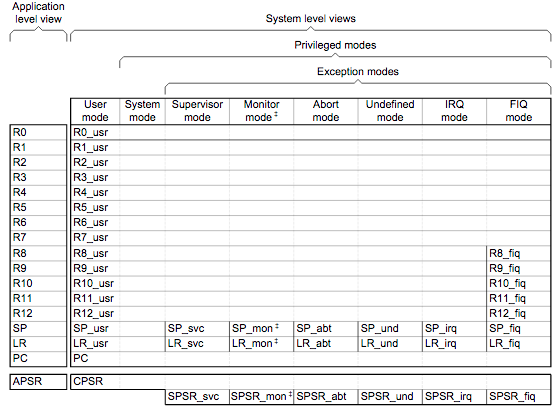
\includegraphics[width=1\textwidth]{includes/figures/chapter2_registers_vs_modes.png}  \\[0.5 cm]
\end{center}
\caption{Registers and Modes summary}
\label{fig:chapter2_registers_vs_modes}
\end{figure}


As explained before, the CPSR is the main register to use for switching state. But in fact, the CPSR is used for a lot more than just mode switching, it has (amongst other) these uses: 

\begin{itemize}
\item Processor mode
\item Thumb enabled/disabled bit
\item FIQ enabled/disabled bit
\item IRQ enabled/disabled bit
\item Data endianness bit
\item Branch state bit (namely IT)
\item Greater-than-or-equal-to bit (namely GE)
\item Do-not-monidify bits (DNM)
\item Carry/borrow/extend bit
\item Zero bit
\item Negative/less than bit
\end{itemize}

This is why it is extremely important to be careful when modifying the CPSR, this is why the ARM is also provided with a SPSR. Also, it is prime importance to save such register when performing context switching. Finally, the CPSR contains reserved bit, as explained in the ARM documentation these registers are currently unused but present for future features. The figure~\ref{fig:chapter2_cpsr} pictures a summary of the bits present in the CPSR in a graphical manner.

\begin{figure}[H]
\begin{center}
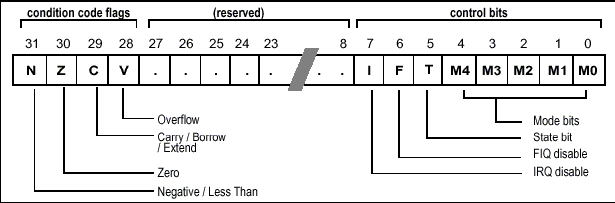
\includegraphics[width=1\textwidth]{includes/figures/chapter2_cpsr.png}  \\[0.5 cm]
\end{center}
\caption{CPSR bits}
\label{fig:chapter2_cpsr}
\end{figure}


\section{Serial Communications}\label{chapter2_serial_communications}
\subsection{Introduction}
The serial communication (as opposed to parallel communication) is the process of sending data one bit a time over a communication channel. This is one of the simplest mean of communication and one of the more used in mainstream computing as for instance USB, SATA and PCIe are all using serial communication within their protocol. The serial communication uses a series of mechanisms that provide error-free transfers across the devices such as synchronization bits (to avoid data loss) and parity bits (for error checking).

Serial communications are all based on a internal clock that has to be known before starting the communication that is called the \emph{baud rate}. The baud (in bits per seconds) specifies how fast data is sent over the serial communication. It is important to know beforehand the baud rate of the communication otherwise it is impossible for the two devices to synchronize and exchange data without errors.

The serial communication being just a concept, the specifics of the protocol such as data framing, synchronization, error checking, etc. are specified by the standard used. The one used in this project is specified in the next section.


\subsection{UART}
UART stands for \textit{Universal Asynchronous Receiver/Transmitter}\cite{uart} and is a computer devices that is used to translate data sent from a parallel way into byte and vice versa. It is therefore required that both ends of the link have a UART devices in order to be able to communicate.

As for many other protocols, UART uses frames to transmit its data, that is, the data that is to be transferred is cut into little chunk which are framed (i.e. placed into sequence of a bit data allows the receiver to know where the boundaries of the data are).
The frame contains:
\begin{itemize}
\item A start bit
\item The data
\item Parity bit (optional)
\item Two stop bits
\end{itemize}

When the communication is idle, all the bits are set HIGH, it therefore comes that the start bit is set to LOW. The parity bit is optional but provide an additional layer of error checking. Finally, the two stop bits are always set to HIGH.


\begin{figure}[H]
\begin{center}
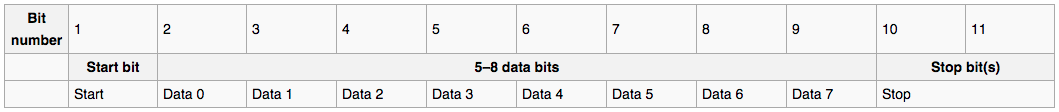
\includegraphics[width=1\textwidth]{includes/figures/chapter2_uart_framing.png}  \\[0.5 cm]
\caption{Schema of a frame in a UART transmission}
\end{center}
\label{fig:chapter2_uart_framing}
\end{figure}

 



\section{Raspberry Pi B+}\label{chapter2_raspberry_pi}
On top of the ARM resides the Raspberry Pi with its set of rules and hardware. For this section, we will focus on the model that is relevant for this project, that is, the Raspberry Pi model B+.

\subsection{Hardware}
The hardware has to be handled by the kernel up to a certain extends. Depending on the hardware, different parameters parameters and protocols are to be employed. This section is a summary of the relevant part of how to use them and how it has been design in the kernel.

In order to gather the information related to a given hardware, the official Broadcom BCM2835 ARM Peripherals manual\cite{arm_peripherals_manual} has be used. It states on page 6:

\begin{displayquote}
Physical addresses range from 0x20000000 to 0x20FFFFFF for peripherals. The bus addresses for peripherals are set up to map onto the peripheral bus address range starting at 0x7E000000. Thus a peripheral advertised here at bus address 0x7Ennnnnn is available at physical address 0x20nnnnnn.
\end{displayquote}

We are going to use the physical address (i.e. from 0x20000000 to 0x20FFFFFF). The peripheral address of the Raspbery Pi can be found with an offset from the base value. For instance, the GPIO address can be found with an offset of 0x200000, the UART with an offset of 0x201000, etc).

The hardware in the scope of this bachelor thesis are the GPIO, the UART and the GPU. We will therefore introduce these components below.

\subsubsection{GPIO}
The GPIO is the easiest way to handles I/O with an external devices, as its name implies. The Raspberry Pi uses a J8 header, that is, a 26-usable-pins GPIO, the other being for the ground or power supply. Finally, there are some GPIO numbers that don't have any physical pins but have influence on the board. For instance, GPIO 47 refers to the ACT LED. The figure~\ref{fig:chapter2_GPIO_pins} is a table presenting the GPIO pins\cite{pi4j}.

\begin{figure}[H]
\begin{center}
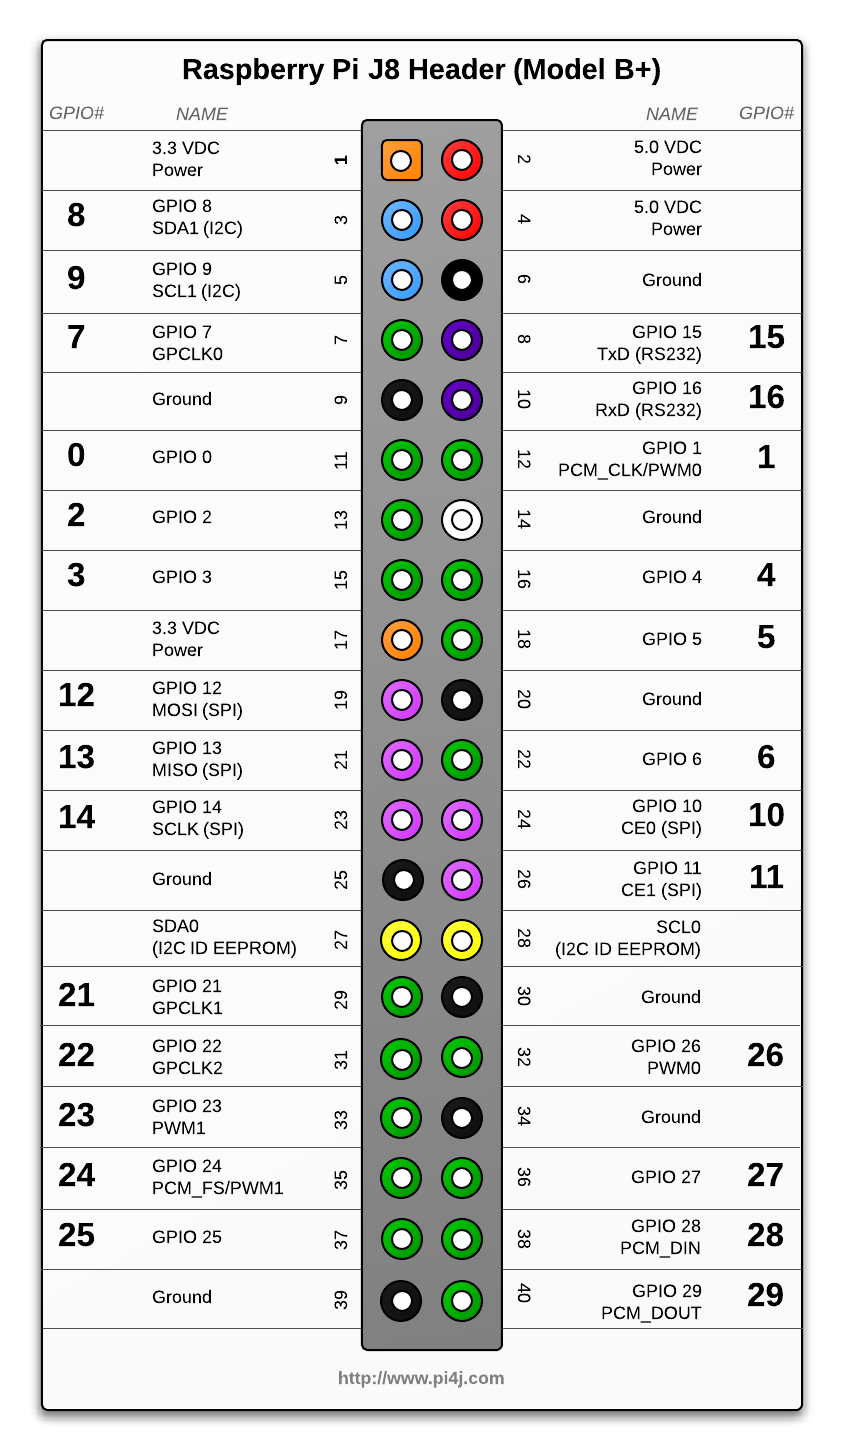
\includegraphics[width=0.4\textwidth]{includes/figures/chapter2_GPIO_pins.png}  \\[0.5 cm]
\end{center}
\caption{GPIO pins of the Raspbery Pi B+}
\label{fig:chapter2_GPIO_pins}
\end{figure}

Only five pins are actually used for the project:
\begin{itemize}
\item\textbf{Pin 2 - 5.0V DC} - This will be the Pin used for providing power to the board.
\item\textbf{Pin 6 - GROUND}
\item\textbf{Pin 8 - TxD} - Transmit data. This is the pin used to output data serially to the computer.
\item\textbf{Pin 10 - RxD} - Receive data. This is the pin used to receive data serially from the computer.
\item\textbf{Pin 47 - ACT LED} - It is possible to turn it on and off, this led is specially useful before having implemented the serial output drivers.
\end{itemize}


The pins 8 and 10 are used for the UART serial communication between the computer and the Raspberry Pi.

\subsubsection{The Message-Handling Unit: The Mailbox}

The mailboxes\cite{mailbox} are a hardware tool that ease the communication between the the ARM processor and the VideoCore. It allows the communication of these two components using asynchronous messages, hence the name 'Mailbox'. It contains seven channels that are each for a different purpose/task:
\begin{itemize}
	\item\textbf{Channel 0}: Power management interface channel
	\item\textbf{Channel 1}: Frame-buffer channel
	\item\textbf{Channel 2}: Virtual UART channel
	\item\textbf{Channel 3}: VCHIQ interface
	\item\textbf{Channel 4}: LEDs interface channel
	\item\textbf{Channel 5}: Buttons interface channel
	\item\textbf{Channel 6}: Touch-screen interface channel
\end{itemize}

All of these mailbox can contain up to \textit{height} messages of 32-bits which can be allocated using a FIFO policy.

The only channel that we will be using for this work is the channel 1, related to the frame-buffer as it will help us to ask for the VideoCore a address where the data related to the screen can be written. Please find the status of the organization of the message hereunder:

\begin{table}[H]
    \centering
    \begin{tabular}{| p{3cm} | p{7cm} |}
    \hline
    \textbf{Byte}	&  \textbf{Meaning} \\ \hline
        0                   &  \textbf{Physical Width}: Width to upscale the virtual width to. \\ \hline
    4                   &  \textbf{Physical Height}: Height to upscale the virtual height to. \\ \hline
    8                   &  \textbf{Virtual Width}: Width of the native frame-buffer \\ \hline
    12                  &  \textbf{Virtual Height}: Height of the native frame-buffer \\ \hline
    16                  &  \textbf{GPU - Pitch} \\ \hline
    20                  &  \textbf{Bit Depth}: How many byte to allocate for each pixel, related to colour depth \\ \hline
    24                  &  \textbf{X}: Number of bits to skip in the top left side on the horizontal axis \\ \hline
    28                  &  \textbf{Y}: Number of bits to skip in the top left side on the vertical axis \\ \hline
    32                  &  \textbf{GPU - Pointer}: Pointer where the frame-buffer is located\\ \hline
    36                  &  \textbf{GPU - Size}: Size of the the frame-buffer in byte\\ \hline
    \end{tabular}
    \caption{Message structure to obtain a frame-buffer from the VideoCore}
\end{table}



\subsection{Booting Process}\label{chapter2_booting_process}
The board is devoid of power button, instead, the Raspberry Pi boots automatically when power is applied to the board. The booting process is a bit atypical as the device that is first powered and that initializes the booting sequence is the VideoCore processor, which start the stage 1 bootstrap from the ROM in the SoC. The stage 1 bootstrap gives the instruction to initialize the SD Card, mount it and start the file bootcode.bin. 
Below is the list of the boot stages:
\begin{enumerate}
  \item\textbf{hardcoded firmware} - This code starts on the GPU, mounts and executes stage 2.
  \item\textbf{bootcode.bin} - Still running on the GPU, it enables the RAM and starts stage 3.
  \item\textbf{start.elf} - This is the firmware of the GPU. It reads the file \textit{config.txt} if any, and starts setting up the GPU. This stage is also in charge of partitioning the RAM into two regions: GPU RAM and CPU RAM, this is set so that the ARM processor will take the leftover RAM. It finally reads another configuration file: \textit{cmdline.txt}, it contains the attributes to be passed to the kernel before starting. Finally, it loads and execute the kernel.img file and start the CPU.
  \item\textbf{kernel.img} - This is the user code, that is, the file that this thesis aims to produce.
\end{enumerate}


Both \textit{bootcode.bin} and \textit{start.elf} can be found on the official repository of the Raspberry Pi\cite{firmware_boot} but they belong to BroadCom that hasn't released the source for those two files and have various feature that are undocumented, which makes custom boot-loaders extremely tedious to produce.

This is the latter that we will implement. It is to be compiled with the arm cross compiler\cite{osdev_raspberry_pi}.

\begin{figure}[H]
\begin{center}
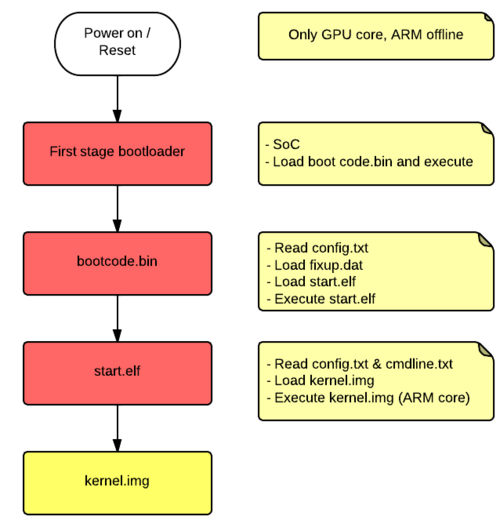
\includegraphics[width=0.5\textwidth]{includes/figures/chapter1_booting_process.png}  \\[0.5 cm]
\caption{Schema representing the boot process}
\end{center}
\end{figure}

\subsubsection{config.txt}
As aforementioned, this file contains parameters that are used to set up the CPU and GPU. A broad range of parameters can be set\cite{config_txt}: from the memory that the GPU will use, disable or enabling the L2 cache, setting up the audio and PWM, setting up the HDMI video mode (video, audio, frequency, resolution, pixel encoding, etc.).

\subsubsection{kernel.img}
This is the user code. The bootloader stage 3 will load that file and by default expect the first instruction to be stored at the address \textit{0x8000}, this is to be taken into account when compiling our kernel.

\subsection{Famous Operating Systems}
Not surprisingly, the most popular OS' on the Raspberry are Linux-based. Here is a non-exhaustive list of the most notable operating system that can be run by the Raspberry Pi:
\begin{itemize}
\item\textbf{Raspbian\cite{raspbian}:} OS based on the highly popular Debian distribution optimized for the Raspberry-Pi. Raspbian is bundled with more than 35000 packages, which allow a very broad set of possibilities (from Desktop use to more specific use for developers. This is the go-to OS for a general purpose Raspberry Pi.

\item\textbf{ArchLinux\cite{archlinux_arm}:} Port of the ArchLinux distribution to ARM processors. It is suited for more specific use as the user can and has to install specific packages that is suited for its use as the basic installation only comes with the Linux kernel, a shell and a package manager.

\item\textbf{OpenELEC\cite{openelec}:} OpenELEC stands for \textit{Open Embedded Linux Entertainment Center}, this is the go-to distribution for using the Raspberry Pi as a media center.

\item\textbf{Kali Linux\cite{kali}:} As for ArchLinux, this is a port of the popular Kali Linux to the ARM processors. This is the distribution of choice for forensics analysis and penetration testing.

\item\textbf{RetroPie\cite{retropie}:}  This distribution is for entertainment purposes as it proposes a wide set of emulator for old consoles proposing a retro gaming experience. The distribution supports game pads for various consoles as long as an adapter is purchased.

\item\textbf{FreeRTOS\cite{freertos}:} Whereas the previous OS are all based on the Linux Kernel, FreeRTOS has its standalone kernel and Operating System specially tailored for real-time purposed for embedded systems
\end{itemize}


\subsection{Raspberry Pi in the Scientific Literature}

Mr \textit{Eric Biggers} wrote a paper regarding the port of Xinu\cite{xinu_biggers}, an Operating System totally independent on UNIX as it has been made without any goal of compatibility and without the knowledge of the source code of UNIX. The paper shows different challenges and solutions brought by Mr. Biggers in order to port it to the Raspberry Pi. Other papers have been publish but are more related to the IoT\footnote{Internet of Things}, it is therefore out of the scope of this document.

\chapter{Developing Environment}

This section is aimed to present the development method as well as the programming language, tools, software and hardware used throughout the development of this bachelor thesis.

The section \ref{chapter3_methodology} introduces the methodology used for developing the kernel.

The section \ref{chapter3_software} introduces the different software and operating systems used in order to compile and use the kernel. In addition to that, the software used for the realisation of the project are also introduced. 


\section {Methodology}\label{chapter3_methodology}

The methodology used for developing the features of the operating system uses the TDD\footnote{Test-Driven Development}\cite{tdd} method. That is, when a feature is needed, a test is made and then the solution is developed. It helps to have a clear idea of the edge cases and what the function should do. Continuous automated testing of the projects offers several key advantages:
\begin{itemize}
\item\textbf{Documentation purposes:} Although it doesn't alone give a complete documentation of the function, it shows clearly how it should be used and why it has been thought for. The scenarios displayed in the tests should be typical scenario that can happen when using them in the project.
\item\textbf{Bug prevention:} A very common way to introduce bug in a library is to change the algorithm while keeping backward compatibility. If the feature has been tested, a developer shouldn't fear to update the internal implementation of a function (for example, improve the efficiency or enhance the results of said function) as the tests will fails if the function doesn't behave any more as it is expected to in at least one of the cases.
\item\textbf{Time saver:} Automated tests are very useful as they allows the developer to avoid testing every cases by hand when modifying a feature. The tests being automated, they will notify failures, if any, automatically. 
\end{itemize}

\begin{figure}
\begin{center}
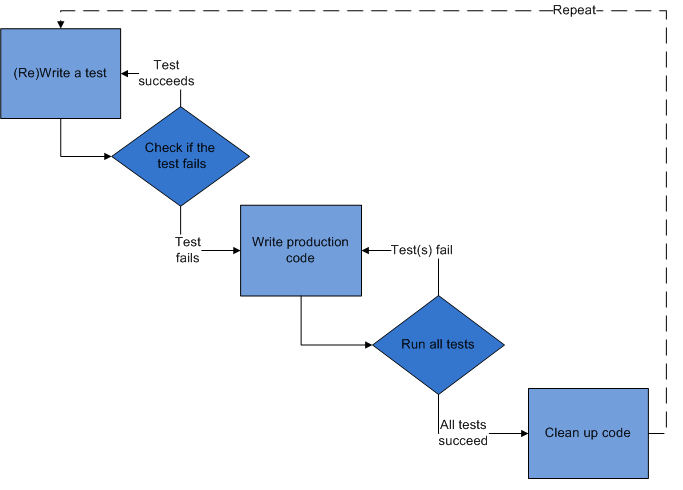
\includegraphics[width=0.5\textwidth]{includes/figures/chapter3_tdd_flowchart.png}  \\[0.5 cm]
\caption{Flowchart of a TDD-driven project}
\end{center}
\end{figure}


In this thesis, a tests have been created in any of these three scenarios:
\begin{itemize}
\item\textbf{Feature creation:} As stated by the TDD, a test should be created before implementing the solution.
\item\textbf{Feature enhancement:} If the algorithm has been changed and some behaviour has been modified, a test is created.
\item\textbf{Bug encountered:} When an unexpected scenario has been found leading to an incorrect behaviour, a test is created testing for the correct behaviour and then the function tested is modified to fit all the previously made tests as well as the newly created one.
\end{itemize}



\section{Software}\label{chapter3_software}

\subsection{Operating System}
The Operating System used for the development, compilation of the kernel and redaction of the documentation is Mac OSX version 10.10. This is the latest iteration of Apple's Operating System.


\subsection{Programming Language}

The end program needs to be compiled to an ARM assembly program, it is therefore all naturally that at the very beginning of the project, the kernel was implemented in ARM Assembly. However, as many people that wrote code in assembly know, assembly can reveal itself tedious to work with, I therefore looked for a way to use either the C or C++ programming languages. However, I've had way more practice with C, especially throughout the whole degree, than C++. It is very difficult to write the whole kernel without any ARM Assembly in it: The bootstrap of the kernel is written in ARM ASM (i.e.: The stack settings as well as the interrupt vector), and the higher level of code is written in C.

Regarding C, it is a general-purpose programming language created in 1972 by Dennis Ritchie and Brian Kernighan\cite{ritchie_c}, however, it is often used for low level programming or programs to be run from within a CLI\footnote{Command line interface}. It has been created to be mapped efficiently to machine code as an alternative to assembly programming, which is one of the main reasons why it is still nowadays a famous programming language for operating system development (Linux, for instance, is almost completely implemented in C).

Due to the popularity and the age of C, it proposed a wide range of advantage:
\begin{itemize}
\item Compatible with most current Operating System
\item Fast and efficient as it is really close to machine code
\item Lot of support and in our case, compiler and cross compilers for a large set of computers.
\item Modulable through the usage of libraries. 
\end{itemize}

As a drawback, C totally lacks of Object-Oriented features (C++ has been created to fix this issue), and it has a steep learning curve.


\subsection{Cross-Compiler}

A cross-compiler is a compiler that is able to create binary code for a machine different that on which the compiler is run. Since the code is not being compiled on the Raspberry Pi but instead, on independent computer, the use of a cross-compiler is mandatory.

In order to compile the kernel, the YAGARTO GNU ARM toolchain\cite{yagarto} has been used. The YAGARTO toolchain was initially made to be executable on Microsoft Windows with the objective to be independent from Cygwin\cite{cygwin}, a Unix-like environment and command-line interface for Microsoft Windows that provides native integration of Windows-based applications, data, and other system resources with applications, software tools, and data of the Unix-like environment. and be cheap for beginner (it is actually free). The YAGARTO project has then be ported to Mac OSX. Amongst other program, this toolchain comes with the following tools that are used for the compilation process:
\begin{itemize}
\item \textbf{arm-none-eabi-as:} Used for the compilation of the assembly code.
\item \textbf{arm-none-eabi-gcc:} Used for the compilation of the C code.
\item \textbf{arm-none-eabi-ld:} Used for the linking of the object files into an ELF\footnote{Executable Linkable Format} file following a given memory map.
\item \textbf{arm-none-eabi-objcopy:} Used to convert the compiled file back to assembly code, it is used mainly for debug purposes.
\end{itemize}


\subsection{Clang}

Clang is an open source compiler for the C, C++, Object-C and Objective C++ programming languages. It uses LLVM\footnote{Low Level Virtual Machine}\cite{llvm} as compiler infrastructure developed by Apple starting from 2007 but that has since then received involvement from other companies such as Google, ARM or even Intel. This is the compiler present by default on the Mac OSX operating system and the one used in this project to compile the code that can be executed by the users for the functional testings. 


\subsection{GNU Screen}

GNU Screen is a command-line application for console multiplexing, allowing a user to have different virtual consoles inside one terminal by the mean of different buffers. It has the particularity to able to be detached (i.e. put in the background) and restored later in time without pausing or closing the programs opened in screen. 
The most interesting feature and the one that is directly linked to this project is that GNU Screen can be used a serial console, that is, it is possible to specify a number of baud and a port so as to communicate with a peripheral. This is therefore, the software that is used for communicating with the Raspberry Pi through the serial connection provided by the GPIO. 


\subsection{Atom}
Atom is GitHub's free open source multi-platform text editor written in node.js and base on Chromium. It is highly customizable and supports a large amount of plug-ins thanks to its built in plug-in manager and has a large  community maintaining them. It has out-of-the-box compatibility with Git. Atom is written on node.js and based on Chromium.
This software was used to write all the source code of the kernel for this project.

\subsection{Git}
Git is a free and open source version control system designed by Linus Torvalds. It is a very widely used tool to develop, backup, and distribute source code. It is really handy when developing a software as the user can create versions of the source code (i.e. commit) as well a go back to some previously created version. This tool has been extensively used throughout the development of the kernel.

\subsection{BitBucket}
BitBucket offers private git repositories (i.e. a storage location from which the source code can be updated and retrieved) for free when applying to the student program. This platform has been used to store the source code of the kernel throughout its development.


\subsection{TexMaker}
TexMaker is the application used to write this document. It is a cross-plateform LaTeX editor and is therefore present on the three major Operating System. TexMaker handles the word-processing part with useful shortcuts, auto-completion and spell-checking, but is also able to compile the LaTeX document to several formats with only one key press. In addition to that, it presents a fairly extensive configuration. 


\subsection{draw.io}
Draw.io is a free online diagram drawing application that allows the user to draw figures such as workflow, charts, UML diagrams, network diagrams, use case diagrams, etc. In addition to that, it has a very good integration with the browser's local storage, Google Drive or Dropbox to provide document persistence. This is the application that has been used to drawn most of the diagrams present in this document.
\chapter{Project Description}

This main purpose of this section is to shape the project by defining needs (requirements) as well as use cases and the development process. This is one of the most important part as the development is entirely shaped based on this section.
The requirement needs to define the feature to be developed. Of course, there are two different perspective in a software project: The user perspective and the system perspective. It is therefore necessary to create requirements for both of these perspectives. Requirements can be classified in different types:
\begin{itemize}
\item\textbf{User Requirements:} Requirements that needs to fulfill feature from the user perspective. These are the requested features with the user's words.
\item\textbf{Functional Requirements:} Requirements from the system perspective. It is testable as it targets very concrete parts and therefore specific enough. There are presented from the engineers words.
\item\textbf{Non Functional Requirements}
\end{itemize}


\section{General Constraints}

The system is to be used on a Raspberry Pi, this therefore give several constraints regarding the kernel. The kernel should work with a modest amount of processing power and in a power efficient manner. Also, it should be able to output information without any monitor plugged in.
Being an operating system, it should be able to run flawlessly for an extended amount of time.

\section{Requirements Specifications}
The requirement specification is is the section where the requirements are formalized. In order to formalize them, we will follow the \textit{IEEE Recommended Practice for Software Requirements Specifications}\cite{ieee_software_requirement_specification} that states what the requirements should address their traget and the way these requirements should be formulated. Therefore, software feature, performances, functional and non functional issues as well design and implementation constraints will be specified. It is also recommended to be:
\begin{itemize}
\item\textbf{Correct:} A requirement is correct if and only if every requirement stated therein is one that the software shall meet.
\item\textbf{Unambiguous:} A requirement is unambiguous if and only if every requirement stated therein has only one interpretation.
\item\textbf{Complete:} A requirement is complete if all significant requirements should be acknowledged and treated. Also, the system's responses should be clearly stated in the valid and invalid case.
\item\textbf{Consistent:} The requirements are consistent if none of them conflict (i.e.: a mutually exclusive behavior).
\item\textbf{Ranked for importance and/or stability:} Each requirements needs to have an identifier reflecting their importance.
\item\textbf{Verifiable:} The requirements need to be verifiable and be able to be checked in a reasonable amount of time, that is, there exists some finite cost-effective process with which a person or machine can check that
the software product meets the given requirement. 
\item\textbf{Modifiable:} A requirement is said to be modifiable if and only if its structure and style are such that any changes to the requirements can be made easily, completely, and consistently while retaining the structure and style.
\item\textbf{Traceable:} A requirement is said to be traceable if and only its origin is clear and can be references in future development stages.
\end{itemize}


In order to fulfill these recommendations and formalize the requirement, we will use a table for each requirements containing the following fields:
\begin{table}[H]
    \centering
    \begin{tabular}{| p{2cm} | p{10cm}|}
    \hline
    \textbf{ID}                 & ID of the requirement\\\hline
    \textbf{Name}               & Name of the requirement\\\hline
    \textbf{Necessity}          & Relevance of the requirement regarding the functionality. the value set to \textit{High}, \textit{Medium} or \textit{Low}\\\hline
    \textbf{Stability}          & Stability (i.e. Relevant) across the whole project. \\\hline
    \textbf{Verifiability}      & Ease to check the requirement. The values can be \textit{Hard}, \textit{Average} or \textit{Easy}\\\hline
    \textbf{Description}       & Description of the requirement following the IEEE recommendations\\\hline
    \textbf{Source}             & On which cycle the requirement has been formalized\\\hline
    \textbf{Priority}           & Importance of the requirement in the final product. The values can be \textit{Critical}, \textit{Conditional} or \textit{Optional} \\\hline
    \end{tabular}
    \caption{Template for the Software Requirements Specification.}
\end{table}


\subsection{User Requirements}

This sections presents the requirements states from a user perspective. These are the feature that the project needs to exhibits when the project is finished.

\begin{table}[H]
    \centering
    \begin{tabular}{| p{2cm} | p{1.6cm} || p{1.6cm}| p{1.6cm} || p{2cm} | p{1.2cm} |}
    \hline
    \textbf{ID}            &  UR-01 & \textbf{Name}         &  \multicolumn{3}{p{4.8cm} |}{Early Outputs}                  \\ \hline
    \textbf{Necessity}     &  High  & \textbf{Priority}     & High & \textbf{Stability}   &   Stable \\ \hline
    \textbf{Verifiability} &  Easy  & \textbf{Source} & \multicolumn{3}{l|}{First} \\ \hline
    \textbf{Description}   & \multicolumn{5}{p{10cm} |}{The system shall be able to output lines while booting giving feedbacks to the users.} \\ \hline
    \end{tabular}
    \caption{User Requirement UR-01: Early Outputs}
    \label{ur01}
\end{table}

\begin{table}[H]
    \centering
    \begin{tabular}{| p{2cm} | p{1.6cm} || p{1.6cm}| p{1.6cm} || p{2cm} | p{1.2cm} |}
    \hline
    \textbf{ID}            &  UR-02 & \textbf{Name}         &  \multicolumn{3}{p{4.8cm} |}{Flash LED when turned ON}                   \\ \hline
    \textbf{Necessity}     &  High  & \textbf{Priority}     & High & \textbf{Stability}   &   Stable \\ \hline
    \textbf{Verifiability} &  Easy  & \textbf{Source} & \multicolumn{3}{l|}{First} \\ \hline
    \textbf{Description}   & \multicolumn{5}{p{10cm} |}{The system shall be able to flash an LED once in a while when turned on.} \\ \hline
    \end{tabular}
    \caption{User Requirement UR-02: Flash LED when turned ON}
    \label{ur02}
\end{table}


\begin{table}[H]
    \centering
    \begin{tabular}{| p{2cm} | p{1.6cm} || p{1.6cm}| p{1.6cm} || p{2cm} | p{1.2cm} |}
    \hline
    \textbf{ID}            &  UR-03 & \textbf{Name}         &  \multicolumn{3}{p{4.8cm} |}{Code Execution}                 \\ \hline
    \textbf{Necessity}     &  High  & \textbf{Priority}     & High & \textbf{Stability}   &   Stable \\ \hline
    \textbf{Verifiability} &  Easy  & \textbf{Source} & \multicolumn{3}{l|}{First} \\ \hline
    \textbf{Description}   & \multicolumn{5}{p{10cm} |}{The system shall be able to execute user function embedded in the kernel.} \\ \hline
    \end{tabular}
    \caption{User Requirement UR-03: Code Execution}
    \label{ur03}
\end{table}


\begin{table}[H]
    \centering
    \begin{tabular}{| p{2cm} | p{1.6cm} || p{1.6cm}| p{1.6cm} || p{2cm} | p{1.2cm} |}
    \hline
    \textbf{ID}            &  UR-04 & \textbf{Name}         &  \multicolumn{3}{p{4.8cm} |}{Input handling}                 \\ \hline
    \textbf{Necessity}     &  High  & \textbf{Priority}     & High & \textbf{Stability}   &   Stable \\ \hline
    \textbf{Verifiability} &  Easy  & \textbf{Source} & \multicolumn{3}{l|}{First} \\ \hline
    \textbf{Description}   & \multicolumn{5}{p{10cm} |}{The system shall be able to receive inputs from a computer and display on the terminal user inputs.} \\ \hline
    \end{tabular}
    \caption{User Requirement UR-04: Input handling}
    \label{ur04}
\end{table}


\begin{table}[H]
    \centering
    \begin{tabular}{| p{2cm} | p{1.6cm} || p{1.6cm}| p{1.6cm} || p{2cm} | p{1.2cm} |}
    \hline
    \textbf{ID}            &  UR-05 & \textbf{Name}         &  \multicolumn{3}{p{4.8cm} |}{HDMI Output}                \\ \hline
    \textbf{Necessity}     &  High  & \textbf{Priority}     & High & \textbf{Stability}   &   Stable \\ \hline
    \textbf{Verifiability} &  Easy  & \textbf{Source} & \multicolumn{3}{l|}{First} \\ \hline
    \textbf{Description}   & \multicolumn{5}{p{10cm} |}{The system shall be able to display an image on a screen using the HDMI connection.} \\ \hline
    \end{tabular}
    \caption{User Requirement UR-05: HDMI Output}
    \label{ur05}
\end{table}


\begin{table}[H]
    \centering
    \begin{tabular}{| p{2cm} | p{1.6cm} || p{1.6cm}| p{1.6cm} || p{2cm} | p{1.2cm} |}
    \hline
    \textbf{ID}            &  UR-06 & \textbf{Name}         &  \multicolumn{3}{p{4.8cm} |}{HDMI Text Output}                   \\ \hline
    \textbf{Necessity}     &  High  & \textbf{Priority}     & High & \textbf{Stability}   &   Stable \\ \hline
    \textbf{Verifiability} &  Easy  & \textbf{Source} & \multicolumn{3}{l|}{First} \\ \hline
    \textbf{Description}   & \multicolumn{5}{p{10cm} |}{The system shall be able to output text on the screen using the HDMI connection.} \\ \hline
    \end{tabular}
    \caption{User Requirement UR-06: HDMI Text Output}
    \label{ur06}
\end{table}


\begin{table}[H]
    \centering
    \begin{tabular}{| p{2cm} | p{1.6cm} || p{1.6cm}| p{1.6cm} || p{2cm} | p{1.2cm} |}
    \hline
    \textbf{ID}            &  UR-07 & \textbf{Name}         &  \multicolumn{3}{p{4.8cm} |}{Debug mode}                 \\ \hline
    \textbf{Necessity}     &  High  & \textbf{Priority}     & High & \textbf{Stability}   &   Stable \\ \hline
    \textbf{Verifiability} &  Easy  & \textbf{Source} & \multicolumn{3}{l|}{First} \\ \hline
    \textbf{Description}   & \multicolumn{5}{p{10cm} |}{The kernel should present the possibility to be run in a debug mode, that is, to display more than the strict necessary feedback for the users and help debug the kernel.} \\ \hline
    \end{tabular}
    \caption{User Requirement UR-07: Debug mode}
    \label{ur07}
\end{table}


\begin{table}[H]
    \centering
    \begin{tabular}{| p{2cm} | p{1.6cm} || p{1.6cm}| p{1.6cm} || p{2cm} | p{1.2cm} |}
    \hline
    \textbf{ID}            &  UR-08 & \textbf{Name}         &  \multicolumn{3}{p{4.8cm} |}{Multitasking}                   \\ \hline
    \textbf{Necessity}     &  High  & \textbf{Priority}     & High & \textbf{Stability}   &   Stable \\ \hline
    \textbf{Verifiability} &  Easy  & \textbf{Source} & \multicolumn{3}{l|}{First} \\ \hline
    \textbf{Description}   & \multicolumn{5}{p{10cm} |}{The system shall be able to execute more than one program at a time.} \\ \hline
    \end{tabular}
    \caption{User Requirement UR-08: Multitasking}
    \label{ur08}
\end{table}


\begin{table}[H]
    \centering
    \begin{tabular}{| p{2cm} | p{1.6cm} || p{1.6cm}| p{1.6cm} || p{2cm} | p{1.2cm} |}
    \hline
    \textbf{ID}            &  UR-09 & \textbf{Name}         &  \multicolumn{3}{p{4.8cm} |}{Command Line Interface}                 \\ \hline
    \textbf{Necessity}     &  High  & \textbf{Priority}     & High & \textbf{Stability}   &   Stable \\ \hline
    \textbf{Verifiability} &  Easy  & \textbf{Source} & \multicolumn{3}{l|}{First} \\ \hline
    \textbf{Description}   & \multicolumn{5}{p{10cm} |}{The system shall be able to offer to the user a CLI\footnote{Command Line Interface} where the user can execute commands and start programs.} \\ \hline
    \end{tabular}
    \caption{User Requirement UR-09: Command Line Interface}
    \label{ur09}
\end{table}



\begin{table}[H]
    \centering
    \begin{tabular}{| p{2cm} | p{1.6cm} || p{1.6cm}| p{1.6cm} || p{2cm} | p{1.2cm} |}
    \hline
    \textbf{ID}            &  UR-10 & \textbf{Name}         &  \multicolumn{3}{p{4.8cm} |}{Standalone kernel}                  \\ \hline
    \textbf{Necessity}     &  High  & \textbf{Priority}     & High & \textbf{Stability}   &   Stable \\ \hline
    \textbf{Verifiability} &  Easy  & \textbf{Source} & \multicolumn{3}{l|}{First} \\ \hline
    \textbf{Description}   & \multicolumn{5}{p{10cm} |}{The system shall use external library only in strictly necessary cases so as to avoid having to adapt the system to a specific framework (ex: Linux).} \\ \hline
    \end{tabular}
    \caption{User Requirement UR-10: Standalone kernel}
    \label{ur10}
\end{table}



\subsection{Functional Requirements}

This sections presents the requirements stated from a system perspective, that is, from a more specific point of view with a more detailed approach.

\begin{table}[H]
    \centering
    \begin{tabular}{| p{2cm} | p{1.6cm} || p{1.6cm}| p{1.6cm} || p{2cm} | p{1.2cm} |}
    \hline
    \textbf{ID}            &  FR-01 & \textbf{Name}         &  \multicolumn{3}{p{4.8cm} |}{Bootloader}                 \\ \hline
    \textbf{Necessity}     &  High  & \textbf{Priority}     & High & \textbf{Stability}   &   Stable \\ \hline
    \textbf{Verifiability} &  Easy  & \textbf{Source} & \multicolumn{3}{l|}{First} \\ \hline
    \textbf{Description}   & \multicolumn{5}{p{10cm} |}{The system shall execute the required instruction to run a hello world program.} \\ \hline
    \end{tabular}
    \caption{Functional Requirement FR-01: bootloader}
    \label{sr01}
\end{table}


\begin{table}[H]
    \centering
    \begin{tabular}{| p{2cm} | p{1.6cm} || p{1.6cm}| p{1.6cm} || p{2cm} | p{1.2cm} |}
    \hline
    \textbf{ID}            &  FR-02 & \textbf{Name}         &  \multicolumn{3}{p{4.8cm} |}{C and ASM language coexistence}                 \\ \hline
    \textbf{Necessity}     &  High  & \textbf{Priority}     & High & \textbf{Stability}   &   Stable \\ \hline
    \textbf{Verifiability} &  Easy  & \textbf{Source} & \multicolumn{3}{l|}{First} \\ \hline
    \textbf{Description}   & \multicolumn{5}{p{10cm} |}{The kernel should offer the possibility to combine ARM ASM language and C language.} \\ \hline
    \end{tabular}
    \caption{Functional Requirement FR-02: C and ASM language coexistence}
    \label{sr02}
\end{table}


\begin{table}[H]
    \centering
    \begin{tabular}{| p{2cm} | p{1.6cm} || p{1.6cm}| p{1.6cm} || p{2cm} | p{1.2cm} |}
    \hline
    \textbf{ID}            &  FR-03 & \textbf{Name}         &  \multicolumn{3}{p{4.8cm} |}{Cross compiler compatibility}                   \\ \hline
    \textbf{Necessity}     &  High  & \textbf{Priority}     & High & \textbf{Stability}   &   Stable \\ \hline
    \textbf{Verifiability} &  Easy  & \textbf{Source} & \multicolumn{3}{l|}{First} \\ \hline
    \textbf{Description}   & \multicolumn{5}{p{10cm} |}{The source code structure shall be compatible with the arm-none-eabi cross-compiler.} \\ \hline
    \end{tabular}
    \caption{Functional Requirement FR-03: Cross compiler compatibility}
    \label{sr03}
\end{table}


\begin{table}[H]
    \centering
    \begin{tabular}{| p{2cm} | p{1.6cm} || p{1.6cm}| p{1.6cm} || p{2cm} | p{1.2cm} |}
    \hline
    \textbf{ID}            &  FR-04 & \textbf{Name}         &  \multicolumn{3}{p{4.8cm} |}{Division and modulo operations support.}                 \\ \hline
    \textbf{Necessity}     &  High  & \textbf{Priority}     & High & \textbf{Stability}   &   Stable \\ \hline
    \textbf{Verifiability} &  Easy  & \textbf{Source} & \multicolumn{3}{l|}{First} \\ \hline
    \textbf{Description}   & \multicolumn{5}{p{10cm} |}{The source code shall implement the missing instructions \_\_aeabi\_uidiv and \_\_aeabi\_uldivmod} \\ \hline
    \end{tabular}
    \caption{Functional Requirement FR-04: Division and modulo operations support}
    \label{sr04}
\end{table}


\begin{table}[H]
    \centering
    \begin{tabular}{| p{2cm} | p{1.6cm} || p{1.6cm}| p{1.6cm} || p{2cm} | p{1.2cm} |}
    \hline
    \textbf{ID}            &  FR-05 & \textbf{Name}         &  \multicolumn{3}{p{4.8cm} |}{ARM Timer interrupt start and stop.}                 \\ \hline
    \textbf{Necessity}     &  High  & \textbf{Priority}     & High & \textbf{Stability}   &   Stable \\ \hline
    \textbf{Verifiability} &  Easy  & \textbf{Source} & \multicolumn{3}{l|}{First} \\ \hline
    \textbf{Description}   & \multicolumn{5}{p{10cm} |}{The kernel shall offer the possibility to start and stop the armtimer interrupt} \\ \hline
    \end{tabular}
    \caption{Functional Requirement FR-05: ARM Timer interrupt start and stop}
    \label{sr05}
\end{table}



\begin{table}[H]
    \centering
    \begin{tabular}{| p{2cm} | p{1.6cm} || p{1.6cm}| p{1.6cm} || p{2cm} | p{1.2cm} |}
    \hline
    \textbf{ID}            &  FR-06 & \textbf{Name}         &  \multicolumn{3}{p{4.8cm} |}{ARM Timer interrupt pre-scaler and threshold.}                   \\ \hline
    \textbf{Necessity}     &  High  & \textbf{Priority}     & High & \textbf{Stability}   &   Stable \\ \hline
    \textbf{Verifiability} &  Easy  & \textbf{Source} & \multicolumn{3}{l|}{First} \\ \hline
    \textbf{Description}   & \multicolumn{5}{p{10cm} |}{The kernel shall offer the possibility to set the pre-scaler of the ARM timer as well as its activation threshold.} \\ \hline
    \end{tabular}
    \caption{Functional Requirement FR-06: ARM Timer interrupt pre-scaler and threshold}
    \label{sr06}
\end{table}


\begin{table}[H]
    \centering
    \begin{tabular}{| p{2cm} | p{1.6cm} || p{1.6cm}| p{1.6cm} || p{2cm} | p{1.2cm} |}
    \hline
    \textbf{ID}            &  FR-07 & \textbf{Name}         &  \multicolumn{3}{p{4.8cm} |}{UART set-up}                \\ \hline
    \textbf{Necessity}     &  High  & \textbf{Priority}     & High & \textbf{Stability}   &   Stable \\ \hline
    \textbf{Verifiability} &  Easy  & \textbf{Source} & \multicolumn{3}{l|}{First} \\ \hline
    \textbf{Description}   & \multicolumn{5}{p{10cm} |}{The kernel shall be able to set up the UART hardware module of the Raspberry Pi.} \\ \hline
    \end{tabular}
    \caption{Functional Requirement FR-07: UART set-up}
    \label{sr07}
\end{table}


\begin{table}[H]
    \centering
    \begin{tabular}{| p{2cm} | p{1.6cm} || p{1.6cm}| p{1.6cm} || p{2cm} | p{1.2cm} |}
    \hline
    \textbf{ID}            &  FR-08 & \textbf{Name}         &  \multicolumn{3}{p{4.8cm} |}{UART output}                \\ \hline
    \textbf{Necessity}     &  High  & \textbf{Priority}     & High & \textbf{Stability}   &   Stable \\ \hline
    \textbf{Verifiability} &  Easy  & \textbf{Source} & \multicolumn{3}{l|}{First} \\ \hline
    \textbf{Description}   & \multicolumn{5}{p{10cm} |}{The kernel shall present a library that allows the developer to send data through the UART serial communication. This library shall be analogous to the Linux's \textit{printf}.} \\ \hline
    \end{tabular}
    \caption{Functional Requirement FR-08: UART output}
    \label{sr08}
\end{table}


\begin{table}[H]
    \centering
    \begin{tabular}{| p{2cm} | p{1.6cm} || p{1.6cm}| p{1.6cm} || p{2cm} | p{1.2cm} |}
    \hline
    \textbf{ID}            &  FR-09 & \textbf{Name}         &  \multicolumn{3}{p{4.8cm} |}{UART input}                 \\ \hline
    \textbf{Necessity}     &  High  & \textbf{Priority}     & High & \textbf{Stability}   &   Stable \\ \hline
    \textbf{Verifiability} &  Easy  & \textbf{Source} & \multicolumn{3}{l|}{First} \\ \hline
    \textbf{Description}   & \multicolumn{5}{p{10cm} |}{The kernel shall present a library that allows the developer to receive data through the UART serial communication. The maximum buffer allowed should be up to 16 bytes a seconds.} \\ \hline
    \end{tabular}
    \caption{Functional Requirement FR-09: UART input}
    \label{sr09}
\end{table}


\begin{table}[H]
    \centering
    \begin{tabular}{| p{2cm} | p{1.6cm} || p{1.6cm}| p{1.6cm} || p{2cm} | p{1.2cm} |}
    \hline
    \textbf{ID}            &  FR-10 & \textbf{Name}         &  \multicolumn{3}{p{4.8cm} |}{UART output debug}                  \\ \hline
    \textbf{Necessity}     &  High  & \textbf{Priority}     & High & \textbf{Stability}   &   Stable \\ \hline
    \textbf{Verifiability} &  Easy  & \textbf{Source} & \multicolumn{3}{l|}{First} \\ \hline
    \textbf{Description}   & \multicolumn{5}{p{10cm} |}{The kernel shall present a function that will only prints when compiled with the DEBUG flag. The function shall be called \textit{print\_debug}.} \\ \hline
    \end{tabular}
    \caption{Functional Requirement FR-10: UART output debug}
    \label{sr10}
\end{table}


\begin{table}[H]
    \centering
    \begin{tabular}{| p{2cm} | p{1.6cm} || p{1.6cm}| p{1.6cm} || p{2cm} | p{1.2cm} |}
    \hline
    \textbf{ID}            &  FR-11 & \textbf{Name}         &  \multicolumn{3}{p{4.8cm} |}{ACT LED}                \\ \hline
    \textbf{Necessity}     &  High  & \textbf{Priority}     & High & \textbf{Stability}   &   Stable \\ \hline
    \textbf{Verifiability} &  Easy  & \textbf{Source} & \multicolumn{3}{l|}{First} \\ \hline
    \textbf{Description}   & \multicolumn{5}{p{10cm} |}{The kernel shall present a function that allows the developer to turn ON or OFF the ACT LED of the Raspberry Pi.} \\ \hline
    \end{tabular}
    \caption{Functional Requirement FR-11: ACT LED}
    \label{sr11}
\end{table}


\begin{table}[H]
    \centering
    \begin{tabular}{| p{2cm} | p{1.6cm} || p{1.6cm}| p{1.6cm} || p{2cm} | p{1.2cm} |}
    \hline
    \textbf{ID}            &  FR-12 & \textbf{Name}         &  \multicolumn{3}{p{4.8cm} |}{ARM Mailbox read}                   \\ \hline
    \textbf{Necessity}     &  High  & \textbf{Priority}     & High & \textbf{Stability}   &   Stable \\ \hline
    \textbf{Verifiability} &  Easy  & \textbf{Source} & \multicolumn{3}{l|}{First} \\ \hline
    \textbf{Description}   & \multicolumn{5}{p{10cm} |}{The kernel shall be able to read any channel of the ARM mailbox.} \\ \hline
    \end{tabular}
    \caption{Functional Requirement FR-12: ARM Mailbox read}
    \label{sr12}
\end{table}


\begin{table}[H]
    \centering
    \begin{tabular}{| p{2cm} | p{1.6cm} || p{1.6cm}| p{1.6cm} || p{2cm} | p{1.2cm} |}
    \hline
    \textbf{ID}            &  FR-13 & \textbf{Name}         &  \multicolumn{3}{p{4.8cm} |}{ARM Mailbox write}                  \\ \hline
    \textbf{Necessity}     &  High  & \textbf{Priority}     & High & \textbf{Stability}   &   Stable \\ \hline
    \textbf{Verifiability} &  Easy  & \textbf{Source} & \multicolumn{3}{l|}{First} \\ \hline
    \textbf{Description}   & \multicolumn{5}{p{10cm} |}{The kernel shall be able to write on any channel of the ARM mailbox.} \\ \hline
    \end{tabular}
    \caption{Functional Requirement FR-13: ARM Mailbox write}
    \label{sr13}
\end{table}


\begin{table}[H]
    \centering
    \begin{tabular}{| p{2cm} | p{1.6cm} || p{1.6cm}| p{1.6cm} || p{2cm} | p{1.2cm} |}
    \hline
    \textbf{ID}            &  FR-14 & \textbf{Name}         & \multicolumn{3}{p{4.8cm} |}{Frame buffer initialization for the HDMI output}                \\ \hline
    \textbf{Necessity}     &  High  & \textbf{Priority}     & High & \textbf{Stability}   &   Stable \\ \hline
    \textbf{Verifiability} &  Easy  & \textbf{Source} & \multicolumn{3}{l|}{First} \\ \hline
    \textbf{Description}   & \multicolumn{5}{p{10cm} |}{The kernel shall be able to initialize the frame buffer interface.} \\ \hline
    \end{tabular}
    \caption{Functional Requirement FR-14: Frame buffer initialization for the HDMI output}
    \label{sr14}
\end{table}


\begin{table}[H]
    \centering
    \begin{tabular}{| p{2cm} | p{1.6cm} || p{1.6cm}| p{1.6cm} || p{2cm} | p{1.2cm} |}
    \hline
    \textbf{ID}            &  FR-15 & \textbf{Name}         &  \multicolumn{3}{p{4.8cm} |}{Draw a pixel on the HDMI}                   \\ \hline
    \textbf{Necessity}     &  High  & \textbf{Priority}     & High & \textbf{Stability}   &   Stable \\ \hline
    \textbf{Verifiability} &  Easy  & \textbf{Source} & \multicolumn{3}{l|}{First} \\ \hline
    \textbf{Description}   & \multicolumn{5}{p{10cm} |}{The kernel shall be able to draw a pixel given a successfully initialized frame buffer, a color and the (x,y) coordinates of said pixel.} \\ \hline
    \end{tabular}
    \caption{Functional Requirement FR-15: Draw a pixel on the HDMI output}
    \label{sr15}
\end{table}


\begin{table}[H]
    \centering
    \begin{tabular}{| p{2cm} | p{1.6cm} || p{1.6cm}| p{1.6cm} || p{2cm} | p{1.2cm} |}
    \hline
    \textbf{ID}            &  FR-16 & \textbf{Name}         &  \multicolumn{3}{p{4.8cm} |}{Draw a line on the HDMI output}                 \\ \hline
    \textbf{Necessity}     &  High  & \textbf{Priority}     & High & \textbf{Stability}   &   Stable \\ \hline
    \textbf{Verifiability} &  Easy  & \textbf{Source} & \multicolumn{3}{l|}{First} \\ \hline
    \textbf{Description}   & \multicolumn{5}{p{10cm} |}{The kernel shall be able to draw a line given a successfully initialized frame buffer, a color and the (x,y) coordinates of the start and end pixels.} \\ \hline
    \end{tabular}
    \caption{Functional Requirement FR-16: Draw a line on the HDMI output}
    \label{sr16}
\end{table}


\begin{table}[H]
    \centering
    \begin{tabular}{| p{2cm} | p{1.6cm} || p{1.6cm}| p{1.6cm} || p{2cm} | p{1.2cm} |}
    \hline
    \textbf{ID}            &  FR-17 & \textbf{Name}         &  \multicolumn{3}{p{4.8cm} |}{Clear the frame buffer of the HDMI output}                  \\ \hline
    \textbf{Necessity}     &  High  & \textbf{Priority}     & High & \textbf{Stability}   &   Stable \\ \hline
    \textbf{Verifiability} &  Easy  & \textbf{Source} & \multicolumn{3}{l|}{First} \\ \hline
    \textbf{Description}   & \multicolumn{5}{p{10cm} |}{The kernel shall be able to clear the screens on the HDMI output.} \\ \hline
    \end{tabular}
    \caption{Functional Requirement FR-17: Clear the frame buffer of the HDMI output}
    \label{sr17}
\end{table}


\begin{table}[H]
    \centering
    \begin{tabular}{| p{2cm} | p{1.6cm} || p{1.6cm}| p{1.6cm} || p{2cm} | p{1.2cm} |}
    \hline
    \textbf{ID}            &  FR-18 & \textbf{Name}         &  \multicolumn{3}{p{4.8cm} |}{Print characters on the HDMI output}                \\ \hline
    \textbf{Necessity}     &  High  & \textbf{Priority}     & High & \textbf{Stability}   &   Stable \\ \hline
    \textbf{Verifiability} &  Easy  & \textbf{Source} & \multicolumn{3}{l|}{First} \\ \hline
    \textbf{Description}   & \multicolumn{5}{p{10cm} |}{The kernel shall exhibit a function that is able to write a full character onto the screen buffer} \\ \hline
    \end{tabular}
    \caption{Functional Requirement FR-18: Print characters on the HDMI output}
    \label{sr18}
\end{table}


\begin{table}[H]
    \centering
    \begin{tabular}{| p{2cm} | p{1.6cm} || p{1.6cm}| p{1.6cm} || p{2cm} | p{1.2cm} |}
    \hline
    \textbf{ID}            &  FR-19 & \textbf{Name}         &  \multicolumn{3}{p{4.8cm} |}{Print strings on the HDMI output}                   \\ \hline
    \textbf{Necessity}     &  High  & \textbf{Priority}     & High & \textbf{Stability}   &   Stable \\ \hline
    \textbf{Verifiability} &  Easy  & \textbf{Source} & \multicolumn{3}{l|}{First} \\ \hline
    \textbf{Description}   & \multicolumn{5}{p{10cm} |}{The kernel shall exhibit a function that is able to write a string using the function defined on the previous requirement.} \\ \hline
    \end{tabular}
    \caption{Functional Requirement FR-19: Print strings on the HDMI output}
    \label{sr19}
\end{table}


\begin{table}[H]
    \centering
    \begin{tabular}{| p{2cm} | p{1.6cm} || p{1.6cm}| p{1.6cm} || p{2cm} | p{1.2cm} |}
    \hline
    \textbf{ID}            &  FR-20 & \textbf{Name}         &  \multicolumn{3}{p{4.8cm} |}{String management library}                   \\ \hline
    \textbf{Necessity}     &  High  & \textbf{Priority}     & High & \textbf{Stability}   &   Stable \\ \hline
    \textbf{Verifiability} &  Easy  & \textbf{Source} & \multicolumn{3}{l|}{First} \\ \hline
    \textbf{Description}   & \multicolumn{5}{p{10cm} |}{The kernel shall exhibit a library dealing with strings. Said library shall have the following functions implemented:
    \begin{itemize}
            \item\textbf{number\_of\_digits:} A function returning the amount of digits a integer has.
        \item\textbf{itoa:} An integer to string function.
        \item\textbf{itoh:} An integer to hexadecimal representation function.
        \item\textbf{sprintf:} Given a destination char pointer, an input char pointer and a set of argument associated to the input string, format said string to include those arguments into the string. The use shall be analogous to Linux's sprintf.
        \item\textbf{rpi\_printf:} Kernel equivalent of Linux's printf. It receives the same inputs than sprintf but also print this string on the serial port.
        \item\textbf{screen\_printf:} Kernel equivalent of Linux's printf. It receives the same inputs than sprintf but also print this string on the HDMI port.
        \item\textbf{rpi\_strlen:} Return the length of a string (i.e.: From the start up to the character).
        \item\textbf{rpi\_strcpy:} Copy the \textit{length}-first characters of a char pointer into a destination char pointer.
        \item\textbf{rpi\_strcmp:} Returns \textit{EQUAL\_STRINGS} if two strings are equals, \textit{DIFFERENT\_STRINGS} else.
        \item\textbf{rpi\_trim:} Copy the content of the input strings into a destination string removing the leading and trailing spaces.
        \item\textbf{get\_first\_word:} Returns the first word found on the input string into the destination string.
    \end{itemize}    
    }
\\ \hline
    \end{tabular}
    \caption{Functional Requirement FR-20: String management library}
    \label{sr20}
\end{table}





\begin{table}[H]
    \centering
    \begin{tabular}{| p{2cm} | p{1.6cm} || p{1.6cm}| p{1.6cm} || p{2cm} | p{1.2cm} |}
    \hline
    \textbf{ID}            &  FR-21 & \textbf{Name}         &  \multicolumn{3}{p{4.8cm} |}{sei and cli}                \\ \hline
    \textbf{Necessity}     &  High  & \textbf{Priority}     & High & \textbf{Stability}   &   Stable \\ \hline
    \textbf{Verifiability} &  Easy  & \textbf{Source} & \multicolumn{3}{l|}{First} \\ \hline
    \textbf{Description}   & \multicolumn{5}{p{10cm} |}{
    Creation of two functions to allow and disallow interrupts:
    \begin{itemize}
        \item\textbf{sei (Set Interrupts)}: Enable interrupts
        \item\textbf{cli (Clear Interrupts)}: Disable interrupts 
    \end{itemize}
    These functions shall be used when a program reaches a critical section.
    }
\\ \hline
    \end{tabular}
    \caption{Functional Requirement FR-21: Sei and cli}
    \label{sr21}
\end{table}


\begin{table}[H]
    \centering
    \begin{tabular}{| p{2cm} | p{1.6cm} || p{1.6cm}| p{1.6cm} || p{2cm} | p{1.2cm} |}
    \hline
    \textbf{ID}            &  FR-22 & \textbf{Name}         &  \multicolumn{3}{p{4.8cm} |}{Memory management library}                \\ \hline
    \textbf{Necessity}     &  High  & \textbf{Priority}     & High & \textbf{Stability}   &   Stable \\ \hline
    \textbf{Verifiability} &  Easy  & \textbf{Source} & \multicolumn{3}{l|}{First} \\ \hline
    \textbf{Description}   & \multicolumn{5}{p{10cm} |}{The kernel shall exhibit a library dealing with the memory. Said library shall have the following functions implemented:
    \begin{itemize}
        \item\textbf{rpi\_memset:} Given a pointer \textit{p}, a length \textit{l} and a byte value \textit{v}, the function shall write l times v from the pointer location onwards. This function is similar to Linux's \textit{memset}.
        \item\textbf{memory\_alloc:} Dynamically allocate a memory chunk of a given length and return the memory's location. This function is similar to Linux's malloc.
        \item\textbf{memory\_free:} Free a memory chunk previously allocated with \textit{memory\_alloc}.
    \end{itemize}    }
\\ \hline
    \end{tabular}
    \caption{Functional Requirement FR-22: Memory management library}
    \label{sr22}
\end{table}




\begin{table}[H]
    \centering
    \begin{tabular}{| p{2cm} | p{1.6cm} || p{1.6cm}| p{1.6cm} || p{2cm} | p{1.2cm} |}
    \hline
    \textbf{ID}            &  FR-23 & \textbf{Name}         &  \multicolumn{3}{p{4.8cm} |}{Interrupt handlers}                \\ \hline
    \textbf{Necessity}     &  High  & \textbf{Priority}     & High & \textbf{Stability}   &   Stable \\ \hline
    \textbf{Verifiability} &  Easy  & \textbf{Source} & \multicolumn{3}{l|}{First} \\ \hline
    \textbf{Description}   & \multicolumn{5}{p{10cm} |}{
    Create an interruption handler for all the different types of interruptions, that is:
    \begin{itemize}
        \item  reset
        \item  undefined instruction vector
        \item  software interrupt vector
        \item  prefetch abort vector
        \item  data abort vector
        \item  unused
        \item  interrupt vector
        \item  fast interrupt vector
    \end{itemize}
    }
\\ \hline
    \end{tabular}
    \caption{Functional Requirement FR-23: Interrupt handlers}
    \label{sr23}
\end{table}



\begin{table}[H]
    \centering
    \begin{tabular}{| p{2cm} | p{1.6cm} || p{1.6cm}| p{1.6cm} || p{2cm} | p{1.2cm} |}
    \hline
    \textbf{ID}            &  FR-24 & \textbf{Name}         &  \multicolumn{3}{p{4.8cm} |}{Threads and contexts}                \\ \hline
    \textbf{Necessity}     &  High  & \textbf{Priority}     & High & \textbf{Stability}   &   Stable \\ \hline
    \textbf{Verifiability} &  Easy  & \textbf{Source} & \multicolumn{3}{l|}{First} \\ \hline
    \textbf{Description}   & \multicolumn{5}{p{10cm} |}{The concept of contexts and thread must be implemented. A context will need to store the link register, the stack pointer and the base stack pointer.}
\\ \hline
    \end{tabular}
    \caption{Functional Requirement FR-24: Threads and contexts}
    \label{sr24}
\end{table}



\begin{table}[H]
    \centering
    \begin{tabular}{| p{2cm} | p{1.6cm} || p{1.6cm}| p{1.6cm} || p{2cm} | p{1.2cm} |}
    \hline
    \textbf{ID}            &  FR-25 & \textbf{Name}         &  \multicolumn{3}{p{4.8cm} |}{Context switching}                \\ \hline
    \textbf{Necessity}     &  High  & \textbf{Priority}     & High & \textbf{Stability}   &   Stable \\ \hline
    \textbf{Verifiability} &  Easy  & \textbf{Source} & \multicolumn{3}{l|}{First} \\ \hline
    \textbf{Description}   & \multicolumn{5}{p{10cm} |}{Context shall be able to be switched. That is, a thread shall be able to get paused and executed at any time thanks to a context switch algorithm. The context switch shall be executed every time a timer interrupt is raised.}
\\ \hline
    \end{tabular}
    \caption{Functional Requirement FR-25: Context switching}
    \label{sr25}
\end{table}


\begin{table}[H]
    \centering
    \begin{tabular}{| p{2cm} | p{1.6cm} || p{1.6cm}| p{1.6cm} || p{2cm} | p{1.2cm} |}
    \hline
    \textbf{ID}            &  FR-26 & \textbf{Name}         &  \multicolumn{3}{p{4.8cm} |}{Thread scheduling}                \\ \hline
    \textbf{Necessity}     &  High  & \textbf{Priority}     & High & \textbf{Stability}   &   Stable \\ \hline
    \textbf{Verifiability} &  Easy  & \textbf{Source} & \multicolumn{3}{l|}{First} \\ \hline
    \textbf{Description}   & \multicolumn{5}{p{10cm} |}{A scheduler shall be implemented. The scheduler shall be called at the moment of a context switch and will decide what is the next thread to be executed. The scheduler shall provide an easy way to change/implement a new scheduling algorithm.}
\\ \hline
    \end{tabular}
    \caption{Functional Requirement FR-26: Thread scheduling}
    \label{sr26}
\end{table}



\begin{table}[H]
    \centering
    \begin{tabular}{| p{2cm} | p{1.6cm} || p{1.6cm}| p{1.6cm} || p{2cm} | p{1.2cm} |}
    \hline
    \textbf{ID}            &  FR-27 & \textbf{Name}         &  \multicolumn{3}{p{4.8cm} |}{Round-robin scheduling}                \\ \hline
    \textbf{Necessity}     &  High  & \textbf{Priority}     & High & \textbf{Stability}   &   Stable \\ \hline
    \textbf{Verifiability} &  Easy  & \textbf{Source} & \multicolumn{3}{l|}{First} \\ \hline
    \textbf{Description}   & \multicolumn{5}{p{10cm} |}{The scheduler shall have provide a round-robin scheduling algorithm.}
\\ \hline
    \end{tabular}
    \caption{Functional Requirement FR-27: Round-robin scheduling}
    \label{sr27}
\end{table}


\begin{table}[H]
    \centering
    \begin{tabular}{| p{2cm} | p{1.6cm} || p{1.6cm}| p{1.6cm} || p{2cm} | p{1.2cm} |}
    \hline
    \textbf{ID}            &  FR-28 & \textbf{Name}         &  \multicolumn{3}{p{4.8cm} |}{Display pictures on HDMI Output}                \\ \hline
    \textbf{Necessity}     &  Medium  & \textbf{Priority}     & Medium & \textbf{Stability}   &   Stable \\ \hline
    \textbf{Verifiability} &  Easy  & \textbf{Source} & \multicolumn{3}{l|}{Second} \\ \hline
    \textbf{Description}   & \multicolumn{5}{p{10cm} |}{The system shall be able to display a picture on the HDMI output using raw data provided at compilation time.}
\\ \hline
    \end{tabular}
    \caption{Functional Requirement FR-28: Display pictures on HDMI Output}
    \label{sr28}
\end{table}


\begin{table}[H]
    \centering
    \begin{tabular}{| p{2cm} | p{1.6cm} || p{1.6cm}| p{1.6cm} || p{2cm} | p{1.2cm} |}
    \hline
    \textbf{ID}            &  FR-29 & \textbf{Name}         &  \multicolumn{3}{p{4.8cm} |}{JPEG image conversion tool}                \\ \hline
    \textbf{Necessity}     &  Medium  & \textbf{Priority}     & Medium & \textbf{Stability}   &   Stable \\ \hline
    \textbf{Verifiability} &  Easy  & \textbf{Source} & \multicolumn{3}{l|}{Second} \\ \hline
    \textbf{Description}   & \multicolumn{5}{p{10cm} |}{A tool shall be provided that converts a JPEG image to data usable by the kernel (please refer the previous requirement for the purposes of the tool).}
\\ \hline
    \end{tabular}
    \caption{Functional Requirement FR-29: JPEG image conversion tool}
    \label{sr29}
\end{table}


\begin{table}[H]
    \centering
    \begin{tabular}{| p{2cm} | p{1.6cm} || p{1.6cm}| p{1.6cm} || p{2cm} | p{1.2cm} |}
    \hline
    \textbf{ID}            &  FR-30 & \textbf{Name}         &  \multicolumn{3}{p{4.8cm} |}{Compilation}                \\ \hline
    \textbf{Necessity}     &  High  & \textbf{Priority}     & High & \textbf{Stability}   &   Stable \\ \hline
    \textbf{Verifiability} &  Easy  & \textbf{Source} & \multicolumn{3}{l|}{Second} \\ \hline
    \textbf{Description}   & \multicolumn{5}{p{10cm} |}{The compilation process should be eased with the use of the 'make' tool. The compilation process shall be properly executed without any error messages. The gcc tags for the compilation shall be \textit{-std=c99 -Wall -Werror -Wextra -Wuninitialized -O2 -nostdlib -nostartfiles -ffreestanding}}
\\ \hline
    \end{tabular}
    \caption{Functional Requirement FR-30: Compilation}
    \label{sr30}
\end{table}


\begin{table}[H]
    \centering
    \begin{tabular}{| p{2cm} | p{1.6cm} || p{1.6cm}| p{1.6cm} || p{2cm} | p{1.2cm} |}
    \hline
    \textbf{ID}            &  FR-31 & \textbf{Name}         &  \multicolumn{3}{p{4.8cm} |}{Activity LED on Context Switch}                \\ \hline
    \textbf{Necessity}     &  High  & \textbf{Priority}     & High & \textbf{Stability}   &   Stable \\ \hline
    \textbf{Verifiability} &  Easy  & \textbf{Source} & \multicolumn{3}{l|}{Second} \\ \hline
    \textbf{Description}   & \multicolumn{5}{p{10cm} |}{The ACT LED light state should be reversed at every context switch.}
\\ \hline
    \end{tabular}
    \caption{Functional Requirement FR-31: Activity LED on Context Switch}
    \label{sr31}
\end{table}


\begin{table}[H]
    \centering
    \begin{tabular}{| p{2cm} | p{1.6cm} || p{1.6cm}| p{1.6cm} || p{2cm} | p{1.2cm} |}
    \hline
    \textbf{ID}            &  FR-32 & \textbf{Name}         &  \multicolumn{3}{p{4.8cm} |}{Command Line Interface} \\ \hline
    \textbf{Necessity}     &  High  & \textbf{Priority}     & High & \textbf{Stability}   &   Stable \\ \hline
    \textbf{Verifiability} &  Easy  & \textbf{Source} & \multicolumn{3}{l|}{Second} \\ \hline
    \textbf{Description}   & \multicolumn{5}{p{10cm} |}{The kernel should prompt include a Command Line Interface where the user is prompted to enter commands and the kernel execute said commands if the command exists}
\\ \hline
    \end{tabular}
    \caption{Functional Requirement FR-32: Command Line Interface}
    \label{sr32}
\end{table}

A traceability matrix showing the correlation of the Functional Requirements and the User Requirements can be found on table~\ref{T:traceability_matrix_fr_vs_ur}



\begin{sidewaystable}
\centering
  \begin{adjustbox}{max width=\textwidth}
  \begin{tabular}{| c | *{32}{c}|}
    \hline
            & FR-01 & FR-02 & FR-03 & FR-04 & FR-05 & FR-06 & FR-07 & FR-08 & FR-09 & FR-10 & FR-11 & FR-12 & FR-13 & FR-14 & FR-15 & FR-16 & FR-17 & FR-18 & FR-19 & FR-20 & FR-21 & FR-22 & FR-23 & FR-24 & FR-25 & FR-26 & FR-27 & FR-28 & FR-29 & FR-30 & FR-31 & FR-32   \\ \hline
    UR-01   &       &       &       &       &       &       & X     & X     &       &       &       &       &       &       &       &       &       &       &       &       &       &       &       &       &       &       &       &       &       &       &       &         \\ \hline
    UR-02   &       &       &       &       &       &       &       &       &       &       &       &       &       &       &       &       &       &       &       &       &       &       &       &       &       &       &       &       &       &       & X     &         \\ \hline
    UR-03   & X     & X     & X     & X     &       &       &       &       &       &       &       &       &       &       &       &       &       &       &       &       &       &       &       &       &       &       &       &       &       & X     &       &         \\ \hline
    UR-04   &       &       &       &       &       & X     &       &       & X     &       & X     &       &       &       &       &       &       &       &       &       &       &       &       &       &       &       &       &       &       &       &       & X       \\ \hline
    UR-05   &       &       &       &       &       &       &       &       &       &       &       &       & X     &       & X     & X     & X     &       &       &       &       &       &       &       &       &       &       &       &       &       &       &         \\ \hline
    UR-06   &       &       &       &       &       &       &       &       &       &       &       &       & X     &       & X     &       &       & X     & X     &       &       &       &       &       &       &       &       & X     & X     &       &       &         \\ \hline
    UR-07   &       &       &       &       &       &       &       &       &       & X     &       &       &       &       &       &       &       &       &       &       &       &       &       &       &       &       &       &       &       &       &       &         \\ \hline
    UR-08   &       &       &       &       &       &       &       &       &       &       &       &       &       &       &       &       &       &       &       &       & X     & X     & X     & X     & X     & X     & X     &       &       &       &       & X       \\ \hline
    UR-09   &       &       &       &       &       &       &       &       &       &       &       &       &       &       &       &       &       &       &       &       &       &       &       &       &       &       &       &       &       &       &       &         \\ \hline
    UR-10   & X     & X     & X     & X     &       &       &       &       &       &       &       &       &       &       &       &       &       &       &       &       &       &       &       &       &       &       &       &       &       & X     &       &        \\ \hline
        \end{tabular}
        \end{adjustbox}                                                                        
\caption{Traceability matrix - Functional Requirement vs User Requirements.}
\label{T:traceability_matrix_fr_vs_ur}
\end{sidewaystable}


\subsection{Use Cases}\label{chapter4_use_cases}
A use case aims to define a goal-oriented interactions between:
\begin{itemize}
\item\textbf{The Actor(s)}: Parties outside of the system that interact with it. They can be a user, a role or another system. Actors have goals and they'll use the system to reach this goal.
\item\textbf{The System}: The system is final product that we are considering. In this case, the kernel.
\end{itemize}

A use case sums up the actors, the goals, the sequence of interaction between the actor(s) and the system as well as the requirements that are considered through this use case.

As well as for the requirement specification, we will use table to help define these user cases. The actor will always be the user interacting with the system, for this very reason, this field will be omitted. The template uses with its field and the description thereof is displayed here-under:


\begin{table}[H]
    \centering
    \begin{tabular}{| p{3cm} | p{7cm} |}
    \hline
    \textbf{ID}             & ID of the use case \\ \hline
    \textbf{Name}           & Name of the use case \\ \hline
    \textbf{Description}    & Description of the use case. \\ \hline
    \textbf{Steps}          & Sequence of events that take place along with the use case. \\ \hline
    \textbf{Pre-conditions} & Condition that are supposed to be fulfilled while considering the use case. \\ \hline
    \textbf{Post-conditions} & Conditions that are necessary for the correct realization of the use case. \\ \hline
    \textbf{Requirements}       & Functional requirements that the use case verifies. \\ \hline
    \end{tabular}
    \caption{Template for the use case description.}
\end{table}


Several kind of messages can be printed on the printed in the serial terminal. The early outputs are always displayed even when the kernel hasn't been compiled with the DEBUG flag. The DEBUG messages are prepended by the 'DEBUG: ' string. Finally, the regular messages from program are printed as such.


\begin{table}[H]
    \centering
    \begin{tabular}{| p{3cm} | p{7cm} |}
    \hline
    \textbf{ID}             & UC-01 \\ \hline
    \textbf{Name}           & System boot \\ \hline
    \textbf{Description}    & The system boot. The following messages are displayed on the screen:
    \begin{itemize}
        \item \textit{UART initialized}
        \item \textit{Initializing frame-buffer}
        \item \textit{Frame-buffer correctly initialized}
        \item \textit{Screen-text correctly initialized}
        \item \textit{Memory correctly initialized}    
    \end{itemize}
    \\ \hline
    \textbf{Steps}          &   \begin{enumerate}
                                    \item Plug UART cable into the Raspberry-Pi
                                    \item Plug UART cable's USB side to the computer
                                    \item Start a screen terminal in serial mode
                                \end{enumerate}
 \\ \hline
    \textbf{Pre-conditions} & Kernel compiled successfully. \\ \hline
    \textbf{Post conditions} & Messages correctly displayed and no other error triggered. \\ \hline
    \textbf{Requirements}       &  FR-01, FR-07, FR-08, FR-12, FR-13, FR-14, FR-22\\ \hline
    \end{tabular}
    \caption{Use Case UC-01: System boot}
\end{table}



\begin{table}[H]
    \centering
    \begin{tabular}{| p{3cm} | p{7cm} |}
    \hline
    \textbf{ID}             & UC-02 \\ \hline
    \textbf{Name}           & Kernel compilation \\ \hline
    \textbf{Description}    & The system compiles with all its core component without any error message. The core source code is implemented with both ASM bits and C bits.\\ \hline
    \textbf{Pre-conditions} &   \begin{itemize}
                                    \item Cross compiler installed.
                                    \item 'make' installed
                                \end{itemize} \\ \hline
    \textbf{Steps}          &   \begin{enumerate}
                                    \item Open terminal
                                    \item Go to the kernel's source code directory
                                    \item Type 'make'
                                \end{enumerate}
 \\ \hline
    \textbf{Post conditions} & Only the compilation messages are printed, no error messages from the compiler or the linker are triggered. \\ \hline
    \textbf{Requirements}       &  FR-02, FR-03, FR-08, FR-30\\ \hline
    \end{tabular}
    \caption{Use Case UC-02: Kernel Compilation}
\end{table}


\begin{table}[H]
    \centering
    \begin{tabular}{| p{3cm} | p{7cm} |}
    \hline
    \textbf{ID}             & UC-03 \\ \hline
    \textbf{Name}           & Debug Output \\ \hline
    \textbf{Description}    & The \textit{print\_debug} function prints DEBUG messages if the kernel has been compiled with the DEBUG flag. The kernel boot up has two debug messages:
	\begin{itemize}
		\item Frame-buffer initialized with physical resolution:1280x1024 and virtual:800x600
		\item Initialization finished. Starting main program.
	\end{itemize}
	\\ \hline
    \textbf{Pre-conditions} &   The code should make use of \textit{print\_debug} \\ \hline
    \textbf{Steps}          &   \begin{enumerate}
                                    \item Open terminal
                                    \item Go to the kernel's source code directory
                                    \item Edit makefile
                                    \item Make sure that DEBUGFLAG is set to '-DDEBUG'
                                    \item Type 'make'
                                    \item Boot the kernel 
                                \end{enumerate}
 \\ \hline
    \textbf{Post conditions} & Only the compilation messages are printed, no error messages from the compiler or the linker are triggered. \\ \hline
    \textbf{Requirements}       &  FR-07, FR-08, FR-10, FR-30\\ \hline
    \end{tabular}
    \caption{Use Case UC-03: Debug Output}
\end{table}



\begin{table}[H]
    \centering
    \begin{tabular}{| p{3cm} | p{7cm} |}
    \hline
    \textbf{ID}             & UC-04 \\ \hline
    \textbf{Name}           & ARM timer interrupt \\ \hline
    \textbf{Description}    & The user can trigger a timer interrupt at regular interval which is handled by the function \textit{interrupt\_vector}
	\\ \hline
    \textbf{Pre-conditions} & - \\ \hline
    \textbf{Steps}          &   \begin{enumerate}
                                    \item Edit the function \textit{main\_program} in file \textit{user\_program.c}
                                    \item Call the function \textit{armtimer\_set} with paramter \textit{0xFF}. This sets the frequency of the interrupts before pre-scaling.
                                    \item Call the function \textit{enable\_armtimer\_irq} 
                                    \item Call the function \textit{armtimer\_enable}. Possible pre-scaler are 256, 16 and 1.
                                    \item Call the function \textit{sei} that will enable the interrupts catch.
                                    \item Edit the function \textit{interrupt\_vector} within the file \textit{interrupts.c}
                                    \item Insert everything that needs to be done at each interrupts. For example, printing something on the serial monitor using \textit{rpi\_printf}.
                                    \item Compile the kernel
                                    \item Boot the kernel
                                    \item Appreciate the timer interruptions thanks to the serial print.
                                \end{enumerate}
 \\ \hline
    \textbf{Post conditions} & The serial outputs are correctly printed. \\ \hline
    \textbf{Requirements}       &  FR-05, FR-06, FR-07, FR-08, FR-22, FR-23, FR-30 \\ \hline
    \end{tabular}
    \caption{Use Case UC-04: ARM timer interrupt}
\end{table}



\begin{table}[H]
    \centering
    \begin{tabular}{| p{3cm} | p{7cm} |}
    \hline
    \textbf{ID}             & UC-05 \\ \hline
    \textbf{Name}           & Context switching \\ \hline
    \textbf{Description}    & This use case makes use of the ability of the kernel to handle threads and switch threads via context switching. The currently developed scheduling algorithm is Round Robin (i.e. Each thread has the time before the next interruption in order of creation before switching back to the first one still running and so forth).
	\\ \hline
    \textbf{Pre-conditions} & - \\ \hline
    \textbf{Steps}          &   \begin{enumerate}
                                    \item Edit the function \textit{main\_program} in file \textit{user\_program.c}
                                    \item Create several functions that will be used as thread handler (i.e. The function that a given thread will execute)
                                    \item Create a thread for each of the function created on the previous step using the function \textit{create\_process()} that accepts as first parameter the name of the function and as second the argument to be passed to it.
                                    \item Start the scheduler by using the function \textit{bootstrap\_scheduler}
                                    \item Compile the kernel
                                    \item Boot the kernel
                                \end{enumerate}
 \\ \hline
    \textbf{Post conditions} & 	Appreciate the example image being outputted on the screen.
    							   	\\ \hline
    \textbf{Requirements}       &  FR-05, FR-06, FR-11, FR-21, FR-22, FR-23, FR-24, FR-25, FR-26, FR-27, FR-30, FR-31 \\ \hline
    \end{tabular}
    \caption{Use Case UC-05: Context Switching}
\end{table}


\begin{table}[H]
    \centering
    \begin{tabular}{| p{3cm} | p{7cm} |}
    \hline
    \textbf{ID}             & UC-06 \\ \hline
    \textbf{Name}           & Display an image on the screen\\ \hline
    \textbf{Description}    & Example of how to show a picture on the screen using the HDMI output. This relies on the fact that \textit{print\_buffer\_example} has an example of picture being displayed.
    						   The picture is stored in \textit{data/uc3m.h} in the ALPHA-RED-GREEN-BLUE format.
	\\ \hline
    \textbf{Pre-conditions} & - \\ \hline
    \textbf{Steps}          &   \begin{enumerate}
                                    \item Call at any time \textit{print\_buffer\_example} if it hasn't been called already
                                    \item Compile the kernel
                                    \item Boot the kernel
                                \end{enumerate}
 \\ \hline
    \textbf{Post conditions} & 	\begin{itemize}
    									\item Appreciate the correct creation of the image data file header.
    									\item Appreciate image being correctly outputted on the screen.
    							   	\end{itemize}
    							   	\\ \hline
    \textbf{Requirements}       &  FR-12, FR-13, FR-14, FR-15, FR-28, FR-30 \\ \hline
    \end{tabular}
    \caption{Use Case UC-06: Display an image on the screen}
\end{table}



\begin{table}[H]
    \centering
    \begin{tabular}{| p{3cm} | p{7cm} |}
    \hline
    \textbf{ID}             & UC-07 \\ \hline
    \textbf{Name}           & Create header picture\\ \hline
    \textbf{Description}    & This use case makes use of the ability of the kernel to handle threads and switch threads via context switching. The currently developed scheduling algorithm is Round Robin (i.e. Each thread has the time before the next interruption in order of creation before switching back to the first one still running and so forth).
	\\ \hline
    \textbf{Pre-conditions} & For the image conversion, it is necessary to have \textit{Python} and \textit{PIL} installed on the computer. \\ \hline
    \textbf{Steps}          &   \begin{enumerate}
                                    \item Run the file \textit{utils/imageconverter.py} with the correct parameters (see help of the script)
                                    \item Place the outputted header in the the source code's \textit{include/data} folder.
                                    \item Import the header where the function that calls the library is implemented.
                                    \item The function needs to use the screenbuffer's \textit{display\_image} function.
                                    \item Compile the kernel
                                    \item Boot the kernel
                                \end{enumerate}
                                An example is showed in the function \textit{print\_buffer\_example}
 \\ \hline
    \textbf{Post conditions} & 	\begin{itemize}
    									\item Appreciate the thread switching back and forth
    									\item Appreciate the ACT LED flashing at each context switching
    							   	\end{itemize}
    							   	\\ \hline
    \textbf{Requirements}       &  FR-29 \\ \hline
    \end{tabular}
    \caption{Use Case UC-07: Create header picture}
\end{table}



\begin{table}[H]
    \centering
    \begin{tabular}{| p{3cm} | p{7cm} |}
    \hline
    \textbf{ID}             & UC-08 \\ \hline
    \textbf{Name}           & Print strings on the serial port\\ \hline
    \textbf{Description}    & Showcases the ability of the kernel to format a string and display it on the serial port
	\\ \hline
    \textbf{Pre-conditions} & - \\ \hline
    \textbf{Steps}          &   \begin{enumerate}
                                    \item Use the function \textit{rpi\_printf} for printing a formatted string on the serial output. Please refer to the documentation for more info on the features implemented.  
                                    \item Compile the kernel
                                    \item Boot the kernel
                                    \item Establish a serial communication with the device
                                \end{enumerate}
 \\ \hline
    \textbf{Post conditions} & 	Appreciate the formatted string being displayed on the serial port.
    							   	\\ \hline
    \textbf{Requirements}       &  FR-01, FR-02, FR-03, FR-08, FR-20 \\ \hline
    \end{tabular}
    \caption{Use Case UC-08: Print strings on the serial port}
\end{table}


\begin{table}[H]
    \centering
    \begin{tabular}{| p{3cm} | p{7cm} |}
    \hline
    \textbf{ID}             & UC-09 \\ \hline
    \textbf{Name}           & Print strings on the HDMI port\\ \hline
    \textbf{Description}    & Showcase the ability of the kernel to format a string and display it on the serial port
	\\ \hline
    \textbf{Pre-conditions} & - \\ \hline
    \textbf{Steps}          &   \begin{enumerate}
                                    \item Use the \textit{st\_print\_string} for printing a string on the serial output. 
                                    \item Compile the kernel
                                    \item Boot the kernel
                                    \item Establish a serial communication with the device
                                \end{enumerate}
 \\ \hline
    \textbf{Post conditions} & 	Appreciate the formatted string being displayed on the HDMI port.
    							   	\\ \hline
    \textbf{Requirements}       &  FR-01, FR-02, FR-03, FR-08, FR-18, FR-19 \\ \hline
    \end{tabular}
    \caption{Use Case UC-09: Print strings on the HDMI port}
\end{table}



\begin{table}[H]
    \centering
    \begin{tabular}{| p{3cm} | p{7cm} |}
    \hline
    \textbf{ID}             & UC-10 \\ \hline
    \textbf{Name}           & Input data handling\\ \hline
    \textbf{Description}    & Use case showcasing the ability of the kernel to receive data from an external device using the UART communication scheme.
	\\ \hline
    \textbf{Pre-conditions} & - \\ \hline
    \textbf{Steps}          &  The function is charge of reading the received data is uart.c's \textit{uart\_get\_input\_buffer}.
    							 \begin{enumerate}
    							 	\item Use the function \textit{uart\_get\_input\_buffer} in a while loop.
    							 	\item Print the returned string from the function to see the input mirrored in the output. We will assume that the \textit{rpi\_printf} function is being used.
                                  \item Compile the kernel
                                	\item Boot the kernel
                                	\item Connect to the kernel with the serial communication
                                	\item Type some character and appreciate these characters being mirrored on the serial port by the kernel.
                                \end{enumerate}
                                An example of this code is used in the \textit{interrupt.c} file in the hardware interrupt handler.
 \\ \hline
    \textbf{Post conditions} & 	Appreciate the typed character being mirrored onto the communication medium.
    							   	\\ \hline
    \textbf{Requirements}       & FR-01, FR-02, FR-03, FR-08, FR-09  \\ \hline
    \end{tabular}
    \caption{Use Case UC-10: Input data handling}
\end{table}


\begin{table}[H]
    \centering
    \begin{tabular}{| p{3cm} | p{7cm} |}
    \hline
    \textbf{ID}             & UC-11 \\ \hline
    \textbf{Name}           & Line drawing\\ \hline
    \textbf{Description}    & Use case showcasing the basics of line drawing. It directly involve using screenbuffer's \textit{draw\_line}.
	\\ \hline
    \textbf{Pre-conditions} & Memory initialized and UART initialized \\ \hline
    \textbf{Steps}          &  The function is charge of reading the received data is screenbuffer.c's \textit{draw\_line}.
    							 \begin{enumerate}
    							 	\item Call anywhere in the code \textit{draw\_line} anywhere in the code.  It takes as first two parameters the x and y coordinate of the first point, then the two next are the x and y coordinate of the second point and the last parameter is the color in which the line is to be drawn.
    							 	\item Compile the kernel
    							 	\item Connect HDMI cable to the device
    							 	\item Boot kernel
                                \end{enumerate}
                                An example of this code can be found in the \textit{screenbuffer.c} file in the function named \textit{print\_rotating\_bar\_example}.
 \\ \hline
    \textbf{Post conditions} & 	Appreciate the line being drawn on the screen.
    							   	\\ \hline
    \textbf{Requirements}       & FR-01, FR-02, FR-03, FR-04, FR-07, FR-08, FR-09, FR-30, FR-32  \\ \hline
    \end{tabular}
    \caption{Use Case UC-11: Line drawing}
\end{table}



\begin{table}[H]
    \centering
    \begin{tabular}{| p{3cm} | p{7cm} |}
    \hline
    \textbf{ID}             & UC-12 \\ \hline
    \textbf{Name}           & Command-Line Interface\\ \hline
    \textbf{Description}    & Showcasing the rudimentary CLI implemented in the kernel.
	\\ \hline
    \textbf{Pre-conditions} & UART initialized \\ \hline
    \textbf{Steps}          &  The function is charge of displaying a CLI is the \textit{command\_line} function in cli.c.
    							 \begin{enumerate}
    							 	\item Use the function \textit{command\_line} anywhere in the code to spawn the CLI.
    							 	\item The function used are to be implemented in that very file and populate in the code via the if chain present in the \textit{command\_line} function.
    							 	\item Compile the kernel
                                	\item Connect to the kernel with the serial communication
    							 	\item Boot kernel
                                	\item Type the function with the arguments (if needed).
                                \end{enumerate}
 \\ \hline
    \textbf{Post conditions} & 	Appreciate the functions being correctly executed under the demands of the user.
    							   	\\ \hline
    \textbf{Requirements}       & FR-01, FR-02, FR-03, FR-04, FR-12, FR-13, FR-14, FR-15, FR-16, FR-17, FR-30\\ \hline
    \end{tabular}
    \caption{Use Case UC-12: Command-Line Interface}
\end{table}


A traceability matrix showing the correlation of the Functional Requirements and the Use Cases can be found on table~\ref{T:traceability_matrix_fr_vs_uc}




\begin{sidewaystable}
\centering
  \begin{tabular}{| c | *{12}{c}|}
    \hline
            & UC-01 & UC-02 & UC-03 & UC-04 & UC-05 & UC-06 & UC-07 & UC-08 & UC-09 & UC-10 & UC-11 & UC-12    \\ \hline
    FR-01   & X     &       &       &       &       &       &       & X     & X     & X     & X     & X        \\ \hline
    FR-02   &       & X     &       &       &       &       &       & X     & X     & X     & X     & X        \\ \hline
    FR-03   &       & X     &       &       &       &       &       & X     & X     & X     & X     & X        \\ \hline
    FR-04   & X     & X     &       &       &       &       &       & X     & X     & X     & X     & X        \\ \hline
    FR-05   &       &       &       & X     & X     &       &       &       &       &       &       &          \\ \hline
    FR-06   &       &       &       & X     & X     &       &       &       &       &       &       &          \\ \hline
    FR-07   & X     &       & X     & X     &       &       &       &       &       &       &       &          \\ \hline
    FR-08   & X     & X     & X     & X     &       &       &       & X     & X     & X     &       & X        \\ \hline
    FR-09   &       &       &       &       &       &       &       &       &       & X     &       & X        \\ \hline
    FR-10   &       &       & X     &       &       &       &       &       &       &       & X     &          \\ \hline
    FR-11   &       &       &       &       & X     &       &       &       &       &       & X     &          \\ \hline
    FR-12   & X     &       &       &       &       & X     &       &       &       &       & X     &          \\ \hline
    FR-13   & X     &       &       &       &       & X     &       &       &       &       & X     &          \\ \hline
    FR-14   & X     &       &       &       &       & X     &       &       &       &       & X     &          \\ \hline
    FR-15   &       &       &       &       &       & X     &       &       &       &       & X     &          \\ \hline
    FR-16   &       &       &       &       &       &       &       &       &       &       & X     &          \\ \hline
    FR-17   &       &       &       &       &       &       &       &       &       &       & X     &          \\ \hline
    FR-18   &       &       &       &       &       &       &       &       & X     &       &       &          \\ \hline
    FR-19   &       &       &       &       &       &       &       &       & X     &       &       &          \\ \hline
    FR-20   &       &       &       &       &       &       &       & X     &       &       &       &          \\ \hline
    FR-21   &       &       &       &       & X     &       &       &       &       &       &       &          \\ \hline
    FR-22   & X     &       &       & X     & X     &       &       &       &       &       &       &          \\ \hline
    FR-23   &       &       &       & X     & X     &       &       &       &       &       &       &          \\ \hline
    FR-24   &       &       &       &       & X     &       &       &       &       &       &       &          \\ \hline
    FR-25   &       &       &       &       & X     &       &       &       &       &       &       &          \\ \hline
    FR-26   &       &       &       &       & X     &       &       &       &       &       &       &          \\ \hline
    FR-27   &       &       &       &       & X     &       &       &       &       &       &       &          \\ \hline
    FR-28   &       &       &       &       &       & X     &       &       &       &       &       &          \\ \hline
    FR-29   &       &       &       &       &       &       &  X    &       &       &       &       &          \\ \hline
    FR-30   &       & X     & X     & X     & X     & X     &       &       &       &       & X     & X        \\ \hline
    FR-31   &       &       &       &       & X     &       &       &       &       &       &       &          \\ \hline
    FR-32   &       &       &       &       &       &       &       &       &       &       &       & X        \\ \hline
        \end{tabular}
\caption{Traceability matrix - Functional Requirement vs Use Cases}
\label{T:traceability_matrix_fr_vs_uc}
\end{sidewaystable}


\pagebreak

\section{Software Development Process}\label{sec:chapter4_software_developemnt_process}

Throughout the realization of this project, the software development process chosen is the spiral life-cycle. This process shares many similarities with the incremental model and allows as the project starts to present tasks that are known from the start and that are to be developed and enhanced throughout the project. The big advantages of this process is to allow a flexible requirement elicitation throughout the project as multiple evaluation phases are being done. In addition to that, the project is started early on in the project allowing the creation of tangible materials from the very beginning.

The \textit{spiral} is a metaphor for an iteration, which contains the following phases:
\begin{itemize}
	\item \textbf{Planning Phase}: This phases focuses on the creation and/or overhaul of the previously set requirements. The objective is to review and adapt the requirements as the project evolves. This is the iteration of this phase that generates the whole set of requirements.
	\item \textbf{Risk Analysis Phase}: Aims to identify the risks and solutions that the current iteration presents in respect to the previous iteration. This allows the creation of alternative solutions and tackles problems early on.
	\item \textbf{Engineering Phase}: Phase where the requirements are developed along with the testings necessary to checks their correct functioning allowing a new iteration to be started on strong bases.
	\item \textbf{Evaluation Phase}: Phase where the customer checks the project up to that point in order to start a new iteration once the needs has been overhauled or new needs are specified.
\end{itemize}

A representation\cite{spiral_development} of this development process can be found on figure~\ref{fig:chapter4_spiral_life_cycle_schema}



\begin{figure}
\begin{center}
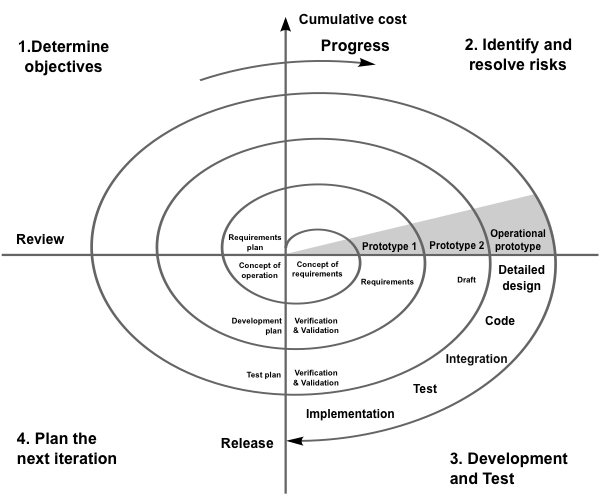
\includegraphics[width=1\textwidth]{includes/figures/chapter4_spiral_life_cycle_schema.png}  \\[0.5 cm]
\end{center}
\caption{Spiral Life-Cycle Schema}
\label{fig:chapter4_spiral_life_cycle_schema}
\end{figure}



The projects will be divided into six cycles, each of them being a particular milestone:
\begin{enumerate}
	\item \textit{Execution of a hello world}: Phase where the first output from the board can be seen.
	\item \textit{Serial output}: Phase aimed to develop the features necessary for printing characters on the serial output of the board and read from an external device.
	\item \textit{HDMI output}: Phase aimed to develop the features necessary for displaying shapes, texts and images on the screen.
	\item \textit{Serial input}: Phase aimed to develop the features necessary for receiving inputs on the board.
	\item \textit{Context Switching}: Phase aimed to develop the features necessary for allowing the kernel to perform context switching and thread scheduling.
	\item \textit{Command line interface}: Phase aimed to develop the feature necessary to present a command line interface to the user.
\end{enumerate}



\chapter{Proposal}

In this section we will set the goals and explain the design and an implementation of the Operating System, that is, the proposed solution to the requirement specifications and use cases presented in the previous chapter. This chapter is divided into two major sections:
\begin{enumerate}
	\item \textbf{Design} This part is about how the system is organized in an abstract way, that is, exposing the different parts of the system, their interactions as well as the design decisions and justification for the these parts.
	\item \textbf{Implementation} This part is the tangible part of the chapter: It shows the organization of the source code, code tree and source code snippets that are relevant for the proposal.
\end{enumerate}

\section{Design}

The design of the kernel is made using three different parts:
\begin{enumerate}
	\item \textbf{The Kernel Core}: The part of the kernel that deal with the hardware at very low level. This part mainly deals with the booting part as well as context switching and interrupts. This part is totally \textbf{architecture dependent}.
	\item \textbf{Kernel management}: Mainly drivers, this part is dedicated to memory management and management of the different hardware part of the Raspberry Pi.
	\item \textbf{Developer API}: This part is not directly needed by the kernel to properly work but it proposes an interface for the developer to use the kernel. It contains modules such as string management module, input/output module, thread module and graphical helper module.
\end{enumerate}


\begin{figure}[H]
\begin{center}
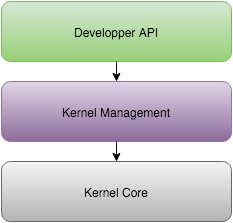
\includegraphics[width=0.5\textwidth]{includes/figures/chapter5_kernel_layers.png}  \\[0.5 cm]
\caption{Kernel layers}
\end{center}
\label{fig:chapter5_kernel_layers}
\end{figure}


\subsection{Kernel Core Layer}
As stated in the introduction, this part of the code is the heavily hardware dependent. It is the one dedicated to the low level interaction with the kernel and is overall dedicated to the CPU and partial interrupt management. Naturally, this part of the kernel is written in ARM assembly language.

This is the first part that has to be executed by the kernel once the Raspberry Pi bootstraping has finished and does in the early part:
\begin{enumerate}
	\item Set-up of the interrupt vector table.
	\item Set-up of the the Interrupt mode's, Fast Interrupt mode's and Supervisor mode's stack pointers.
	\item Jump to the very first bit of the C kernel code (Kernel management layer).
\end{enumerate}


It is also has two essential method that are dedicated to enabling and disabling interrupts.


This layer is indispensable for being able to boot code that is not programmed in assembly and also to handle interrupts in a later stage of the booting process, thanks to the set up of the interrupt vector table and setting up their stack pointers.



\subsection{Kernel Management Layer}
The kernel management is the part that contains different driver modules for the management of the different hardware part of the device. Each of these module have a different tasks that are separated by their main goals.

The diagram below shows the different modules present in this layer as well as their relations between each other. Some of them can be useful on their own (such as the malloc module or the queue module) and can therefore be used by the developer. Some other are only useful for a specific goal (such as the mailbox module, UART module or scheduler module).

\begin{figure}[H]
\begin{center}
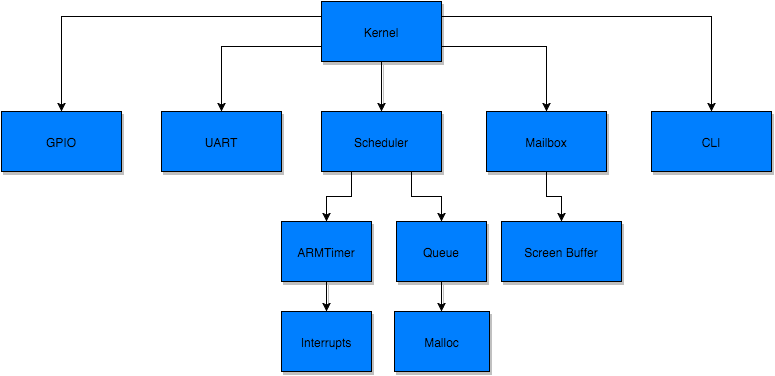
\includegraphics[width=1\textwidth]{includes/figures/chapter5_kernel_management_layer.png}  \\[0.5 cm]
\caption{Kernel Management Layers}
\end{center}
\label{fig:chapter5_kernel_management_layer}
\end{figure}


In the following section we will proceed to present each of these module by defining their goals and what the functions that are to be present.
 are
\subsubsection{Kernel module}
The kernel module is the conductor of the whole kernel. It does nothing by itself but instead manage all the required module for the correct initialization of the kernel and keeps sure that everything has been correctly initialized. After all the booting process, it finally runs the \textit{user program}, that is, the part of the code that is defined by the user. 

\begin{figure}[H]
\begin{center}
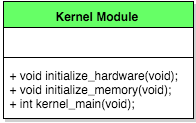
\includegraphics[width=0.4\textwidth]{includes/figures/chapter5_kernel_management_layer_kernel_UML.png}  \\
\caption{Kernel Management Layers - Kernel UML}
\end{center}
\label{fig:chapter5_kernel_management_layer_kernel_UML}
\end{figure}


As displayed on the UML graph, the kernel module has three functions:
\begin{itemize}
	\item \textbf{initialize\_hardware}: Aimed to initialize the UART as well as the frame-buffer for the HDMI outputs.
	\item \textbf{initialize\_memory}: Aimed to initialize the memory needed to use the malloc functions suite.
	\item \textbf{kernel\_main}: This is the function that is called after the kernel initilization (i.e. at the end of the Kernel core sequence). It calls the two previous functions.
\end{itemize}




\subsubsection{GPIO module}

\begin{figure}[H]
\begin{center}
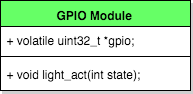
\includegraphics[width=0.4\textwidth]{includes/figures/chapter5_kernel_management_layer_GPIO_UML.png}  \\
\caption{Kernel Management Layers - GPIO UML}
\end{center}
\label{fig:chapter5_kernel_management_layer_GPIO_UML}
\end{figure}


As displayed on the UML graph, the GPIO module has only one functions: The light\_act function. This function is aimed to turn ON or OFF the ACT LED.
However, the important part of that module is that is had to define the constants and the variable required to manipulate said GPIO.




\subsubsection{UART module}

\begin{figure}[H]
\begin{center}
\includegraphics[width=0.4\textwidth]{includes/figures/chapter5_kernel_management_layer_UART_UML.png}  \\
\caption{Kernel Management Layers - UART UML}
\end{center}
\label{fig:chapter5_kernel_management_layer_UART_UML}
\end{figure}


As displayed on the UML graph, the kernel module has five functions:
\begin{itemize}
	\item \textbf{uart\_write\_char}: Aimed to send a byte to the UART hardware. It is typically to write a character.
	\item \textbf{uart\_write}: Aimed to send an array of byte to the UART hardware. It is typically to write a string by recursively called \textit{uart\_write\_char}
	\item \textbf{uart\_read}: Aimed to receive a byte from the UART hardware.
	\item \textbf{uart\_init}: Realize a sequence of instruction aimed to set up the UART communication. It is it to set up the BAUD rate, storing policy, etc.
	\item \textbf{uart\_get\_input\_buffer}: Empty the UART buffer and returns its content to the caller.
\end{itemize}





\subsubsection{Scheduler module}

\begin{figure}[H]
\begin{center}
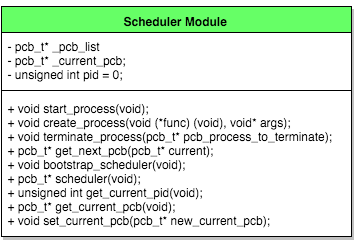
\includegraphics[width=0.7\textwidth]{includes/figures/chapter5_kernel_management_layer_scheduler_UML.png}  \\
\caption{Kernel Management Layers - Scheduler UML}
\end{center}
\label{fig:chapter5_kernel_management_layer_scheduler_UML}
\end{figure}


This module is the biggest and the most complex module in term of code and covers many different features as it handle everything from the context structure declaration up to the scheduler algorithm and the context switching. An important element that is the pillar of this module is the \textit{pcb\_list}. This is a queue (see the queue module) that contains the list of the ready-to-start and started processes. Let's detail all the functions and what their purpose is:
\begin{itemize}
	\item \textbf{create\_process}: This function is in charge of creating a process, that is, creating its metaphor (a PCB \footnote{Process Control Block}), dedicating dynamically its stack memory (see the malloc module), setting up its state and finally inserting the created PCB to the \textit{pcb\_list}.
	\item \textbf{start\_process}: As indicated by its name, it starts a previously created process. When a process is created, it is allocated in memory and the metaphor is initialized with the adequate initial values. Start\_process takes a PCB as parameter and start the process that the PCB refers to.
	\item \textbf{terminate\_process}: This function takes also a PCB as parameter. It terminates the process that the PCB refers to, that is, cleaning the memory related to process (its stack and the PCB structure itself).
	\item \textbf{get\_next\_pcb}: Returns the PCB of the next executable process (i.e. newly created or paused due to a context switch). This is the function mainly used for the Round-Robin scheduling algorithm.
	\item \textbf{scheduler}: This function is to be called to get the next PCB to schedule. In the current design, it simply calls \textit{get\_next\_pcb}, but it is aimed to be able to call any other function depending on the algorithm that the user wants to develop.
	\item \textbf{get\_current\_pid}: System function that a process can run to get its PID\footnote{Process ID, typically an integer that uniquely defines a process}.
	\item \textbf{get\_current\_pcb}: Function that returns the whole PCB of the process currently scheduled to the caller.
	\item \textbf{set\_current\_pcb}: Set the current PCB, that is, the PCB that will be scheduled next.
	\item \textbf{bootstrap\_scheduler}: System function that can be called in order to start the scheduling process, that is: enable the interrupt, set up the ARM timer and ARM timer interrupt, start the first process in the PCB list. This function has to be called only once and assumes that at least one process ready to be scheduled has been inserted into the PCB list.
	\item \textbf{set\_current\_pcb}: Set the current PCB, that is, the PCB that will be scheduled next.
\end{itemize}



\subsubsection{ARMTimer module}


\begin{figure}[H]
\begin{center}
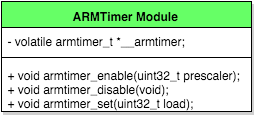
\includegraphics[width=0.5\textwidth]{includes/figures/chapter5_kernel_management_layer_ARMTimer_UML.png}  \\
\caption{Kernel Management Layers - ARMTimer UML}
\end{center}
\label{fig:chapter5_kernel_management_layer_ARMTimer_UML}
\end{figure}


This module is a simple one that is aimed to set up the ARMTimer as well as its interrupt. It only contains three functions:
\begin{itemize}
	\item \textbf{armtimer\_enable}: Enable the timer: Enable the interrupt and set its pre-scaler, that is the amount of cycle that have to be reach to decrement the counter of the timer by one. Once the timer reaches \textit{zero}, an interrupt is triggered. The starting value of the counter is set by the function \textit{armtimer\_set}.
	\item \textbf{armtimer\_disable}: Disable the timer interrupts.
	\item \textbf{armtimer\_set}: Set the timer initial value to the argument that is passed to the function. 
\end{itemize}




\subsubsection{Interrupts module}

\begin{figure}[H]
\begin{center}
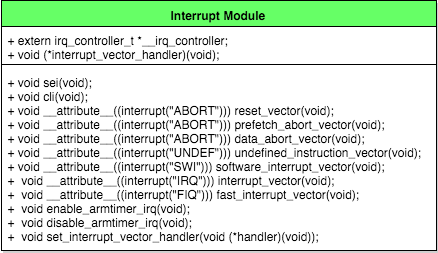
\includegraphics[width=0.7\textwidth]{includes/figures/chapter5_kernel_management_layer_interrupts_UML.png}  \\[0.5 cm]
\caption{Kernel Management Layers - Interrupts UML}
\end{center}
\label{fig:chapter5_kernel_management_layer_interrupts_UML}
\end{figure}

As its name suggests, this class is where the interrupt handlings are made. It has one function for each interrupt but several or them are actually not used in this kernel but are needed to be defined nontheless. It also contains functions that can enable or disable the interrupts handling. All these function are explained below:

\begin{itemize}
	\item \textbf{sei}: Enable the interrupt handling. That is, if an interrupt is triggered, the kernel will execute the appropriate handler.
	\item \textbf{cli}: Disable the interrupt handling. That is, if an interrupt is triggered, no handler will be executed. This functions mainly used for critical sections (i.e.: Sections that shouldn't be interrupted).
	\item \textbf{reset\_vector}: Handler that is triggered during the reset flavour of the \textit{ABORT} interrupt.
	\item \textbf{prefetch\_abort\_vector}: Handler that is triggered during the prefect abort flavour of the \textit{ABORT} interrupt. This handler is not implemented.
	\item \textbf{data\_abort}: Handler that is triggered during the data abort flavour of the \textit{ABORT} interrupt. This interrupt is triggered when having a data fault in the kernel. The interrupt shows a debug message in order to pinpoint the address of the instruction that triggered the data abort interrupt and then cause the kernel to hang.
	\item \textbf{undefined\_instruction\_vector}: Handler that is triggered during an \textit{UNDEF} interrupt. This handler is not implemented.
	\item \textbf{software\_interrupt\_vector}: Handler that is triggered during an \textit{SWI} interrupt (software interrupt). This handler is not implemented as no function trigger software interrupts are implemented.
	\item \textbf{interrupt\_vector}: Handler that is triggered during an \textit{IRQ} interrupt (hardware interrupts). This the interrupt in charge of performing the tasks to be performed at each interrupt generated by the ARMTimer. It is design to read the input received on the UART, and then perform the scheduling and context switch to the next process.
	\item \textbf{fast\_interupt\_vector}: Handler that is triggered during an \textit{FIQ} interrupt (fast interrupt). This handler is not implemented.
	\item \textbf{enable\_armtimer\_irq}: Enable specifically the arm interrupts.
	\item \textbf{disable\_armtimer\_irq}: Disable specifically the arm interrupts.
\end{itemize}


\subsubsection{Queue module}


\begin{figure}[H]
\begin{center}
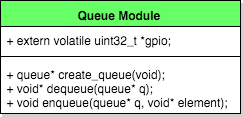
\includegraphics[width=0.5\textwidth]{includes/figures/chapter5_kernel_management_layer_queue_UML.png}  \\
\caption{Kernel Management Layers - Queue UML}
\end{center}
\label{fig:chapter5_kernel_management_layer_queue_UML}
\end{figure}

This module basically defines and handle the queue data structure. A queue is a linear data structure. This data structure present a head and a tail with an element that linked to the next (if any) by storing its value. A queue is always processed from the head to the tail: The next element to be dequeued is the element on the head and when adding an element, it becomes the next tail, this makes it a FIFO\footnote{First-In First-Out} data structure.
It only contains three functions:
\begin{itemize}
	\item \textbf{create\_queue}: It simply create the queue data structure that can then be used with the \textit{dequeue} and \textit{enqueue} functions.
	\item \textbf{dequeue}: As aformentioned, deleting the head of the queue and returning the element in contains. The element that was next to the head is now the new head.
	\item \textbf{enqueue}: This function add an element to the queue and place it right after the tail of the queue, becoming the new tail of the queue.
\end{itemize}


\subsubsection{Malloc module}


\begin{figure}[H]
\begin{center}
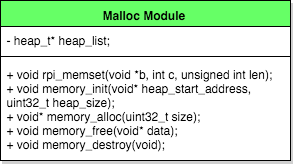
\includegraphics[width=0.6\textwidth]{includes/figures/chapter5_kernel_management_layer_malloc_UML.png}  \\
\caption{Kernel Management Layers - Malloc UML}
\end{center}
\label{fig:chapter5_kernel_management_layer_malloc_UML}
\end{figure}

This module is aimed to provide support to dynamics memory allocation, that is, allocate memory of a dynamic size at run time instead of using the compiler to allocate memory at compile time. This module is specially useful when creating process for the PCB allocation as well at the stack allocation. The specifics of this module are explained in the dedicated part implementation section.
Many function are purposely named at their UNIX counterpart as they mimic their behaviour. The list of the function of this module is described hereafter:
\begin{itemize}
	\item \textbf{rpi\_memset}: It has the same behaviour that you'd expect from the UNIX's \textit{memset}, that is, given a memory address, a value and a length, the function fills the memory address by the value provided and for a number of bytes provided by the length.
	\item \textbf{memory\_init}: This function is needed to be called first before being able to use \textit{memory\_alloc}. Given a memory segment (an address and a length) that will be dedicated to dynamic memory, it creates a \textit{queue} where each element represents a dynamic memory allocation (or a freed one that my be used for another memory allocation).
	\item \textbf{memory\_alloc}: This the kernel's version of UNIX's \textit{malloc}. Given a length in byte, it returns the starting address of a memory segment of the length provided to the function.
	\item \textbf{memory\_free}: Free a memory segment so as to be useful for another memory allocation later in time.
	\item \textbf{memory\_destroy}: This is the reverse of the function \textit{memory\_init}: It frees all the memory segment allocated in the dynamic memory segment and then destroys said memory segment.
\end{itemize}


\subsubsection{Mailbox module}


\begin{figure}[H]
\begin{center}
\includegraphics[width=0.6\textwidth]{includes/figures/chapter5_kernel_management_layer_mailbox_UML.png}  \\
\caption{Kernel Management Layers - Mailbox UML}
\end{center}
\label{fig:chapter5_kernel_management_layer_mailbox_UML}
\end{figure}

The Mailbox module creates the data structure to manipulate the Raspberry's mailbox with ease as well as method that are able to write and read the mailbox according to the board's specifications. It contains only two functions:
\begin{itemize}
	\item \textbf{mailbox\_write}: Given a channel number and an octet of data, sends the provided data to the mailbox on the given channel. 
	\item \textbf{mailbox\_read}: Given a channel, read data from a channel and returns it if any.
\end{itemize}


\subsection{CLI module}
\begin{figure}[H]
\begin{center}
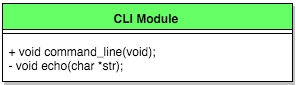
\includegraphics[width=0.6\textwidth]{includes/figures/chapter5_kernel_management_layer_cli_UML.png}  \\
\caption{Kernel Management Layers - CLI UML}
\end{center}
\label{fig:chapter5_kernel_management_layer_mailbox_UML}
\end{figure}

The CLI is the module made for user interactions. The module, as its name suggests, is designed to be able to interpret user's input and execute different commands. Here, only the part made to retrieve the inputs from the user, be able to get the function to run (first word) and pass the argument to the function (is the function is recognized, the arguments is what is directly placed after the function). For now, only the \textit{echo} function is being implemented.
\begin{itemize}
	\item \textbf{command\_line}: Spawn the CLI. When the function is run, is shows a command prompt and asks for the user to enter a command. 
	\item \textbf{echo}: Function available for the CLI. It simply mirrors to the serial interface what has been passed as argument.
\end{itemize}

\pagebreak



\subsection{Developer API Layer}
The developer API layer is the layer that is a lot higher level than the previous Kernel Management Layer. The four modules included into this layer are not considered as the necessary parts of the kernel to work but are nonetheless handy while developing other module, debugging or creating new interactions. As a result, these modules are lot more hardware-independent (unlike the ones from the Kernel Management Layer). This part also contains modules that were developed in a later stage of the project. This sections is here to present these modules.

Although these modules are a lot less interdependent, some of them still depend on others. This is the case of the Screen Text module that depends on the character module and the Standard Input/Output that depends on the Strings module.
Below is a presentation of these four modules: 




\subsubsection{Character module}

\begin{figure}[H]
\begin{center}
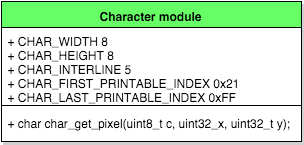
\includegraphics[width=0.6\textwidth]{includes/figures/chapter5_developper_api_layer_char_UML.png}  \\
\caption{Developper API Layer - Character UML}
\end{center}
\label{fig:chapter5_developper_api_layer_char_UML}
\end{figure}

This module is very simple yet very handy. It helps the Screen Text module to print character of the HDMI monitor without having to worry about the type face and the pixels to be printed. The only function of this module, \textit{char\_get\_pixel}, is able to return given a character, a x and y position within the dimensions of the font, the pixel color of the character.




\subsubsection{Screen Text module}

\begin{figure}[H]
\begin{center}
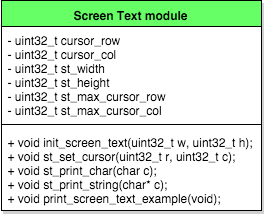
\includegraphics[width=0.6\textwidth]{includes/figures/chapter5_developper_api_layer_st_UML.png}  \\
\caption{Developper API Layer - Screen Text UML}
\end{center}
\label{fig:chapter5_developper_api_layer_st_UML}
\end{figure}

This module is in charge of displaying character on the HDMI output. It keeps track of the pointer and handles jump line. It is directly dependent on the \textit{Character module}. The function that it comprises are the following:
\begin{itemize}
	\item \textbf{init\_screen\_text}: Initializes the screen text (i.e. set the applicable width and height in pixel as well as setting the cursor boundaries).
	\item \textbf{st\_set\_cursor}: Sets the cursor to a given line and column.
	\item \textbf{st\_print\_char}: Prints a character on the current cursor position and update the cursor's position. This is the part that depends on the Character module.
	\item \textbf{st\_print\_string}: Recursively call the \textit{st\_print\_char} character so as to be able to print a string.
	\item \textbf{print\_screen\_text\_example}: Example of how to use the module. Use for presentation or testing purposes.
\end{itemize}




\subsubsection{Strings module}

\begin{figure}[H]
\begin{center}
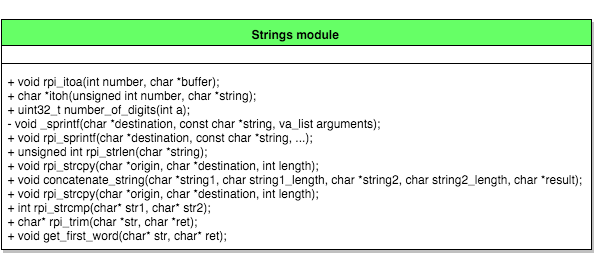
\includegraphics[width=1\textwidth]{includes/figures/chapter5_developper_api_layer_strings_UML.png}  \\
\caption{Developper API Layer - Strings UML}
\end{center}
\label{fig:chapter5_developper_api_layer_strings_UML}
\end{figure}

This module is similar to UNIX's \textit{string} library. This module is capable of handling several strings manipulations. The functions that it implements are described below:
\begin{itemize}
	\item \textbf{number\_of\_digits}: Given an integer, it returns the number of character needed to print said integer.
	\item \textbf{rpi\_itoa}: Integer to string function - Given a number and a character pointer, write the string representation of the number into the character pointer.
	\item \textbf{itoh}: Integer to hexadecimal function - Given a number and a character pointer, write the hexadecimal representation of the number into the character pointer.
	\item \textbf{\_sprintf}: Internal function of the \textit{sprintf} function described below. Given a character pointer (aimed to be the destination), a string with variable place holders and a list of arguments, writes into the destination the formatted string in relation to the arguments.
	\item \textbf{sprintf}: Function consuming the \textit{\_sprintf}. It takes care of the variable number of arguments handling before passing them the \textit{\_sprintf}.
	\item \textbf{rpi\_strlen}: Given a null-ended string, returns its length (i.e.: Number of character until meeting the \textit{null} character).
	\item \textbf{rpi\_strcpy}: Given an origin and a destination char pointer as well as a length, copy the \textit{length} first characters of the origin to the destination.
	\item \textbf{concatenate\_string}: Given a first string, its length, a second string, its length and a destination string (that is assumed to have a length bigger than the sum of the two previous strings), writes the concatenation of the two strings to the destination.
    \item\textbf{rpi\_strcmp:} Returns \textit{EQUAL\_STRINGS} if two strings are equals, \textit{DIFFERENT\_STRINGS} else.
    \item\textbf{rpi\_trim:} Copies the content of the input strings into a destination string removing the leading and trailing spaces.
    \item\textbf{get\_first\_word:} Returns the first word found on the input string into the destination string.
\end{itemize}





\subsubsection{Standard Input/Output}

\begin{figure}[H]
\begin{center}
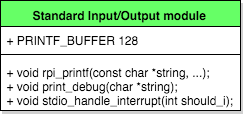
\includegraphics[width=0.5\textwidth]{includes/figures/chapter5_developper_api_layer_stdio_UML.png}  \\
\caption{Developper API Layer - Strings UML}
\end{center}
\label{fig:chapter5_developper_api_layer_stdio_UML}
\end{figure}

The Sandard Input/Output module is in charge of providing some standard API for printing on the serial port. It has three functions:
\begin{itemize}
	\item \textbf{rpi\_printf}: Homologous function of the widely known UNIX \textit{printf} function adapted for this kernel. It internally uses \textit{sprintf} to format the string and then prints said string on the serial port using the UART module.
	\item \textbf{print\_debug}: Function that prints a given string onto the serial port if and only if the kernel has been compiled with the \textit{DEBUG} flag.
	\item \textbf{stdio\_handle\_interrupt}: It is important that this functions of this module are not interrupted (via any kind of interrupt) while they are being executed. This is due to the interaction with the serial port as well as the data that it contains that might be switched be replaced by another thread's argument. Not taking care of the interrupt while using either of the previously mentioned method can trigger a data abort interruption.
\end{itemize}


\pagebreak




\section{Implementation}
This part is aimed to present the tangible part of the project, that is, the source code. It also presents the hierarchy of the project as well as presenting the implementation of some components that are deemed necessary to be explained.

\subsection{Source code tree}
The source code tree is the organization of the source code, that is the folder organization of the code, how the code is structured, and explaining the reasoning being such structure.

Below is the directory tree of the source code with on the right-hand side of the directory or file, a description of its purpose:

\begin{figure}[H]
\dirtree{%
.1 /.
.2 Makefile \hspace{1.1cm} \ldots{}
             \begin{minipage}[t]{10cm}
                Makefile of the whole project{.} An extended description thereof can be found below{.}
            \end{minipage}.
.2 boot/ \hspace{1.65cm} \ldots{}
             \begin{minipage}[t]{10cm}
                Contains all the file that need to be copied the SD card{.}
            \end{minipage}.
.2 include/ \hspace{1.1cm} \ldots{}
             \begin{minipage}[t]{10cm}
                Contains the header files{.}
            \end{minipage}.
.3 data/ \hspace{1.15cm} \ldots{}
             \begin{minipage}[t]{10cm}
                Contains additional data such as pictures or fonts{.}
            \end{minipage}.
.2 linker\_map.s \hspace{0.35cm} \ldots{}
             \begin{minipage}[t]{10cm}
                Linker data for the compilation{.}
            \end{minipage}.
.2 memory\_map.d \hspace{0.35cm} \ldots{}
             \begin{minipage}[t]{10cm}
                Internal memory organization of the executable{.}
            \end{minipage}.
.2 obj/ \hspace{1.85cm} \ldots{}
             \begin{minipage}[t]{10cm}
                Temporary storage of the {.}o files{.}
            \end{minipage}.
.2 src/ \hspace{1.85cm} \ldots{}
             \begin{minipage}[t]{10cm}
                Folder containing the {.}c files{.}
            \end{minipage}.
.3 tests/ \hspace{1cm} \ldots{}
             \begin{minipage}[t]{10cm}
                Folder containing the unitary and functional tests{.} An extended description can be found in the Testing section{.}
            \end{minipage}.
.3 Makefile .
.3 obj/ .
.3 run\_test.sh \hspace{0.05cm} \ldots{}
             \begin{minipage}[t]{10cm}
                Bash script that runs all the tests at once{.}
            \end{minipage}.
.3 src/ \hspace{1.35cm} \ldots{}
             \begin{minipage}[t]{10cm}
                {.}c files of the tests{.}
            \end{minipage}.
}
\caption{Source tree}
\end{figure}


\subsection{Makefile}
The Makefile is the special text file format that allows the mapping of rules to commands as well as command dependency (i.e. a command needs to have its dependencies fulfilled before said command can be run). This is the method that has been chosen for this project for the compilation of the kernel as well as some handy functions that are useful for the user. The more interesting commands and what is their effect while using the Makefile are presented below:
\begin{itemize}
	\item \texttt{make all}: Same as doing both \texttt{make bootfiles} and \texttt{make gcc}\cite{osdev_rpi_bare_bone}
	\item \texttt{make bootfiles}: Download using \textit{curl} the latest boot-files from the official rapsberry-pi repository and store these files into the \textbf{./boot} folder.
	\item \texttt{make gcc}: Compile the project's kernel and place it into the \textbf{./boot} folder.
	\item \texttt{make deploy}: Copy the \textit{kernel.img} file previously compiled with \texttt{make gcc} and place it into the SD Card. It then prints both SHA values to be sure that the kernel has been correctly copied. Please note that this command may vary from one machine to another and might need customization.
	\item \texttt{make connect}: Connect to the raspberry-pi using screen and the baud-rate used in the kernel. It assume that \textit{screen} is installed on the system. Please note that as well as the previous command, the command might need to be adjusted on the machine.
\end{itemize}


\subsection{Booting process of the kernel}
While starting the Raspberry Pi, its own boot-loader is executed, this process has been explained on subsection \ref{chapter2_booting_process} - Booting Process. In this section we are going to talk about the kernel's boot-process, that is, the initialisation of our kernel once the Raspberry Pi is executing the custom code (i.e.: the one we compiled).

Below is a sequence diagram showing the booting process of the kernel from the moment the Raspberry Pi starts executing the code of the kernel up to the moment it executes the main program (that is, the user's code).


\begin{figure}[H]
\begin{center}
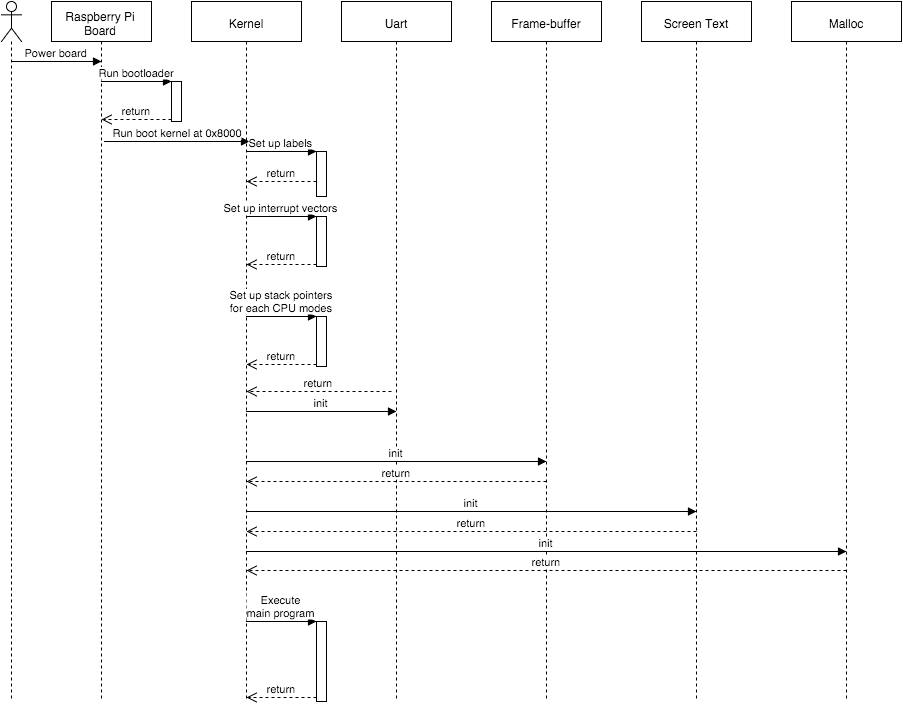
\includegraphics[width=1\textwidth]{includes/figures/chapter5_kernel_booting_sequence.png}  \\
\caption{Kernel Booting Sequence - Sequence Diagram}
\end{center}
\label{fig:chapter5_kernel_booting_sequence}
\end{figure}





\subsection{Dynamic memory allocation}
As aforementioned, dynamic memory allocation is something that is not only expected to be handled by the Operating System but also needed for its functioning. It allow the allocation of memory segments by a program without prior knowledge of how many bytes have to be allocated and how many memory segments will be allocated during the life cycle of the operating system execution. This sections explains how this has been implemented in this project.

Let's first begin by introducing the memory structure that has been chosen for the memory allocation. The heap is a single-linked queue with the following data structure:

\lstset{language=C}
\begin{figure}[H]
\begin{minipage}{\linewidth}
\begin{lstlisting}[frame=single]
struct heap_t
{
    char   size;          // Size of the allocated memory chunk
    char   allocated;     // Is it currently allocated or has it been freed?
    struct heap_t *next;  // Next element in the single-linked queue
};
\end{lstlisting}
\end{minipage}
\caption{Heap data structure}
\end{figure}

Each of the components of these elements is critical for the right functioning of heap. Let's details them:
\begin{itemize}
	\item \textbf{size}: This is the size of the chunk. It helps a lot in conjunction to the variable \textit{allocated} as it allow later memory allocation when the size is inferior than or equal to a previous dynamic memory chunk that has been freed.
	\item \textbf{allocated}: Gives information on whether or not the current chunk is being used (value \textit{ALLOCATED}) or freed (value \textit{UNALLOCATED}) and therefore eligible for a subsequent allocating on this particular memory chunk.
	\item \textbf{next}: The pointer to the next \textit{heap\_t} element in the heap.
\end{itemize}

A representation of the heap memory can be found bellow. It showcases the aforementioned data structure and the writable memory.

\begin{figure}[H]
\begin{center}
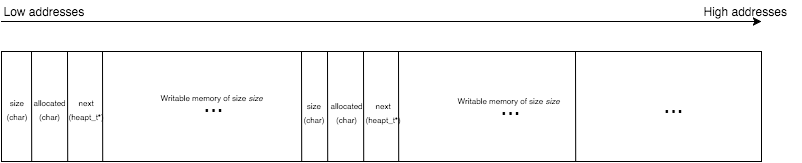
\includegraphics[width=1\textwidth]{includes/figures/chapter5_heap_representation.png}  \\
\caption{Representation of the heap}
\end{center}
\label{fig:chapter5_heap_representation}
\end{figure}

During the introduction to the malloc module, we presented the function \textit{memory\_init}. This function is the one readying the heap of the kernel for memory allocation, that is, it stores the starting value of the heap and write 0 for as long as the length allow us to (this is to ensure no garbage values in the memory heap).

The \textit{memory\_alloc} function is the one that does all the management on whether or not a memory can be allocated on a given memory chunk. It's pseudo-code is presented below.

\lstset{language=C}
\begin{figure}[H]
\begin{minipage}{\linewidth}
\begin{lstlisting}[frame=single]
void* memory_alloc(uint32_t size) {
    h = get_heap_start()    // Memory address of the elected chunk
    if (h != 0) do // First memory allocation
        while true do
            if h > heap_limit OR ((h == NULL OR h->allocated == UNALLOCATED) do
                break
            else
                h = h->next
            done
        done
    done
    
    if h > heap_limit do // Heap full
        return NULL 
    done
    
    // We have a valid chunk
    h->size = size;
    h->allocated = allocated;
    write_zeros_on_writable_memory(h)
    
    if h->next == NULL do
        h->next = h + sizeof(heap_t) + size
    done
    
    
    return h + sizeof(heap_t)   // Return the address of the writable memory
}
\end{lstlisting}
\end{minipage}
\caption{Heap data structure}
\end{figure}


What the function does is basically to iterate through the linked list and find either an eligible chunk or reach the end of the heap by checking the \textit{heap\_limit} variable. In case of failure, the function returns \textit{NULL}, and in case of success, the function returns the address of the writable memory.

In terms of complexity, we are iterating through the whole linked list. So the time complexity of the algorithm is $O(n)$.




\subsection{Context Switching}
Context switching is one of the key parts of this kernel and of an Operating System in general as one is expected to implement multi-tasking. In order to understand the implementation, let's first introduce how context are stored by presenting the data structure thereof. A snippet of the kernel code can be found on figure \ref{fig:chapter5_context_pcb_data_structure}.

As we can see, two figure are set. The first one is the context structure, it is aimed to store the information of a process at a given time. It store the stack pointer as well as the link pointer. Also, it store the original address of the stack pointer. This is needed in order to be able to destroy the memory segment of the stack pointer once we can to destroy the whole process. We can then find the structure of the Process Control Block, that is, the information related to the process in general (ID, its current state, the function that it runs, etc.).

\lstset{language=C}
\begin{figure}[H]
\begin{minipage}{\linewidth}
\begin{lstlisting}[frame=single]
typedef enum {NEW, READY, RUNNING, WAITING, TERMINATED} State;

// Definition of a context
typedef struct {
    unsigned int* sp_origin; // Origin of the stack pointer,
                             // needed for context destruction
    unsigned int* sp;        // Stack pointer
    unsigned int* lr;        // Link register
} context_t;


// Definition of the process control block
struct pcb_t {
    unsigned int  pid;                 // Process indentifier
    State         state;               // State of the process (new, ready, etc.)
    unsigned int  priority;            //The lower the more priority, linux convention
    void          (*function) (void);  // Function that the process will run
    void*         arguments;           // Arguments to be passed to the function
    context_t     context;
    struct pcb_t  *next;               // Next PCB in the single list
};
\end{lstlisting}
\end{minipage}
\caption{Presentation of Context and PCB data structure}
\label{fig:chapter5_context_pcb_data_structure}
\end{figure}


The part of the code dedicated to performing that context switch is present inside the function \textit{interrupt\_vector} inside the \textit{interrupts.c} file. Most of the code prior to that context switch is dedicated to choosing the next PCB to and therefor the next process that will be switched. As stated by the requirement specification, the policy used for the scheduling is Round Robin without priority, that is, the PCB are chosen with the order they have been added to the PCB list and are all allocated a fixed amount of time.

\begin{figure}[H]
\begin{center}
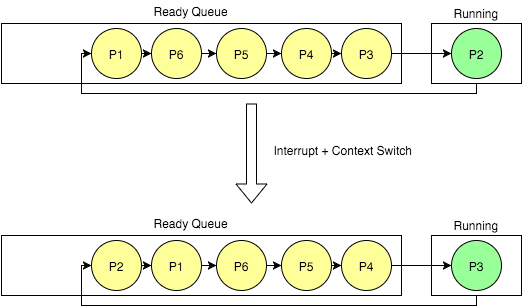
\includegraphics[width=0.8\textwidth]{includes/figures/chapter5_round_robidn_diagram.png}  \\
\caption{Implementation - Diagram of Round Robin without priority}
\end{center}
\label{fig:chapter5_round_robidn_diagram}
\end{figure}



Once the PCB has been chosen, the CPU state is switched to program mode, the register R1 to R12 pushed into the stack. Then the stack pointer and link pointer of the process that was running prior to the interruption is stopped is stored into its context, and the state in the PCB table is changed to \textit{READY}. Immediately after, the context are switched and the switched context is now ready to be run when the interrupts finishes.

Please find on figure \ref{fig:chapter5_snippet_context_switch} the relevant code snippet in charge of performing the context switch.

\begin{figure}[H]
\begin{minipage}{\linewidth}
\begin{lstlisting}[frame=single]
if (current_pcb != NULL) {
    __asm("cps #0x13"); // Switch to program mode in order to access the registers and stack pointer
    __asm("push {r0-r12}");
    __asm("mov %0, sp" : "=r" (current_pcb->context.sp));
    __asm("mov %0, lr" : "=r" (current_pcb->context.lr));
}

// Restore saved context
__asm("mov sp, %0" :: "r" (pcb_to_switch->context.sp));
__asm("mov lr, %0" :: "r" (pcb_to_switch->context.lr));
if (pcb_to_switch->state != NEW) {
    __asm("pop {r0-r12}");
}
\end{lstlisting}
\end{minipage}
\caption{Snippet presenting the context switch}
\label{fig:chapter5_snippet_context_switch}
\end{figure}


\chapter{Testing}

Across the whole development, two kind of testings has been used. It has been mentioned in the project description that a TDD was being used. Of course, this is not possible to perform unit or functional testing on the Kernel Core level due to the big amount of low-level interaction with board mostly performed in assembly. However, the test driven development has been performed on components of the Kernel Management Layer and Developper API. In addition to unit and functional testing, a process of manual testing has been performed, that is, testing the program manually through a series of use cases. The use cases performed for the testing are the exact same than the one described on section \ref{chapter4_use_cases} - Use Cases.

The purpose of this chapter is the present the different tests performed as well as their outcome (i.e. If the tests passed or not).


\section{Functional testing}

Unit and functional testing are two kind of testing method. The Unit testing (also referred as white box testing) is the fact of testing a single function and any call to an external function/module has to be mocked. Functional testing (referred as black box testing) is the fact of testing a function as well as all the internal call as well. The function is tested by knowing what should be the outcome of calling such function with a given input on a given state and testing these outcomes.

In order to perform to tests, a small library has been implemented that enable different kind of assertion as well as error counting and stack tracing (in order to know where the error has occurred). This library has been implemented in the file named \textit{base\_test.c} and present the following assertion:
\begin{itemize}
	\item \textbf{assert\_equals\_integer}: Takes two integer parameters and triggers an error if those two integers aren't equal.
	\item \textbf{assert\_not\_equals\_integer}: Takes two integer parameters and triggers an error if those two integers are equal.
	\item \textbf{assert\_equals\_string}: Takes two string parameters and triggers an error if those two strings aren't equal.
\end{itemize}

The library doesn't have any way of mocking variable or patching function call. Also some tests can look unitary (mainly the one testing stand-alone function that do not need the call of other function), we will also refer to those tests are functional tests.

The source code of the tests are placed under the directory \textit{tests/} and following the following nomenclature:

\textit{X\_test.c} where X is the name of the module being tested.

During this section, the tests will be presented using the table below:

\begin{table}[H]
    \centering
    \begin{tabular}{| p{3cm} | p{7cm} |}
    \hline
    \textbf{ID}             & ID of the functional test.\\ \hline
    \textbf{Name}           & Name of the function in the test file.\\ \hline
    \textbf{Description}    & Description of the feature(s) being tested. \\ \hline
    \textbf{Post-conditions} & Conditions that are necessary for the correct realization of the functional test. \\ \hline
    \textbf{Result}			 & Whether the test passed and fulfilled the post conditions.	 \\ \hline
    \end{tabular}
    \caption{Template for the functional testing.}
\end{table}


Below is the presentation of the performed tests for the given modules:


\edef\functionalTestCounter{0}

\subsection{Malloc}

\pgfmathparse{\functionalTestCounter + 1}
\pgfmathtruncatemacro{\functionalTestCounter}{\pgfmathresult}
\begin{table}[H]
    \centering
    \begin{tabular}{| p{3cm} | p{7cm} |}
    \hline
    \textbf{ID}             & FT-\functionalTestCounter\\ \hline
    \textbf{Name}           & memory\_test\_init \\ \hline
    \textbf{Description}    & Test the function \textit{memory\_init}. The test first call the previous function and check for the correct value of \textit{heap\_top}, \textit{heap\_limit} and the \textit{heap\_list} \\ \hline
    \textbf{Post-conditions} & 
    	\begin{itemize}
    	    	\item \textit{heap\_top} needs to be equal to the initial value of the heap
    	    	\item \textit{heap\_limit} needs to be equal to the value of \textit{heap + 1024} (since 1KiB of data has been ask to \textit{memory\_init}
    	    	\item \textit{heap\_list} needs to be set to zero as no dynamic allocation has been performed for now.
    	\end{itemize}
    \\ \hline
    \textbf{Result}			 & \textcolor{mygreen}{Passed}	 \\ \hline
    \end{tabular}
    \caption{Functional Test FT-\functionalTestCounter: memory\_test\_init}
\end{table}


\pgfmathparse{\functionalTestCounter + 1}
\pgfmathtruncatemacro{\functionalTestCounter}{\pgfmathresult}
\begin{table}[H]
    \centering
    \begin{tabular}{| p{3cm} | p{7cm} |}
    \hline
    \textbf{ID}             & FT-\functionalTestCounter\\ \hline
    \textbf{Name}           & memory\_test\_free\_and\_alloc \\ \hline
    \textbf{Description}    & The feature being tested is the ability to reallocated a block that has been freed if the memory allocation asked is small than or equal to the freed block. To do so, five memory segments are allocated, the fourth one is freed and another memory segments is freed with a size lower than the freed memory segment.\\ \hline
    \textbf{Post-conditions} & The memory address of the memory header of last memory segments allocated needs to be the same as the one that has been freed and the size has to be updated.  \\ \hline
    \textbf{Result}			 & \textcolor{mygreen}{Passed}	\\ \hline
    \end{tabular}
    \caption{Functional Test FT-\functionalTestCounter: memory\_test\_free\_and\_alloc}
\end{table}



\pgfmathparse{\functionalTestCounter + 1}
\pgfmathtruncatemacro{\functionalTestCounter}{\pgfmathresult}
\begin{table}[H]
    \centering
    \begin{tabular}{| p{3cm} | p{7cm} |}
    \hline
    \textbf{ID}             & FT-\functionalTestCounter\\ \hline
    \textbf{Name}           & memory\_test\_four\_alloc \\ \hline
    \textbf{Description}    & After calling \textit{memory\_init}, four allocations are performed. After each of these allocation, tests are performed to check the correct value of the assigned block, the memory address returned and the correct reachability of the block from the \textit{heap\_top} \\ \hline
    \textbf{Post-conditions} &
    	At each allocation, the following tests are performed: 
		\begin{itemize}
			\item \textit{heap\_list} is not null (since an allocation has been performed)
			\item The correct value has been returned by the \textit{memory\_alloc} function (i.e. The address of the writable memory).
			\item The size of the control block of the returned writable memory has the \textit{allocated} field, the \textit{size} field and the \textit{next} correctly set.
		\end{itemize}		    	
    \\ \hline
    \textbf{Result}			 & \textcolor{mygreen}{Passed}	 \\ \hline

    \end{tabular}
    \caption{Functional Test FT-\functionalTestCounter: memory\_test\_four\_alloc}
\end{table}


\pgfmathparse{\functionalTestCounter + 1}
\pgfmathtruncatemacro{\functionalTestCounter}{\pgfmathresult}
\begin{table}[H]
    \centering
    \begin{tabular}{| p{3cm} | p{7cm} |}
    \hline
    \textbf{ID}             & FT-\functionalTestCounter\\ \hline
    \textbf{Name}           & memset\_test \\ \hline
    \textbf{Description}    & Test of the function \textit{rpi\_memset} on a memory segment previously allocated. \\ \hline
    \textbf{Post-conditions} & The memory needs to be correctly set to the value specified to the function on the memory address specified and for the provided length.  \\ \hline
    \textbf{Result}			 & \textcolor{mygreen}{Passed}	\\ \hline

    \end{tabular}
    \caption{Functional Test FT-\functionalTestCounter: memset\_test}
\end{table}






\subsection{Strings}

\pgfmathparse{\functionalTestCounter + 1}
\pgfmathtruncatemacro{\functionalTestCounter}{\pgfmathresult}
\begin{table}[H]
    \centering
    \begin{tabular}{| p{3cm} | p{7cm} |}
    \hline
    \textbf{ID}             & FT-\functionalTestCounter\\ \hline
    \textbf{Name}           & itoa\_test \\ \hline
    \textbf{Description}    & Test of the function \textit{rpi\_itoa} on a positive and a negative value. \\ \hline
    \textbf{Post-conditions} & Correct string representation of the passed value whether it is positive or negative.  \\ \hline
    \textbf{Result}			 & \textcolor{mygreen}{Passed}	\\ \hline

    \end{tabular}
    \caption{Functional Test FT-\functionalTestCounter: itoa\_test}
\end{table}


\pgfmathparse{\functionalTestCounter + 1}
\pgfmathtruncatemacro{\functionalTestCounter}{\pgfmathresult}
\begin{table}[H]
    \centering
    \begin{tabular}{| p{3cm} | p{7cm} |}
    \hline
    \textbf{ID}             & FT-\functionalTestCounter\\ \hline
    \textbf{Name}           & rpi\_strlen\_test \\ \hline
    \textbf{Description}    & Test of the function \textit{rpi\_strlen} with two null-ended strings, one being empty and the other having a non null number of characters. \\ \hline
    \textbf{Post-conditions} & Correct count of character of both string.  \\ \hline
    \textbf{Result}			 & \textcolor{mygreen}{Passed}	\\ \hline

    \end{tabular}
    \caption{Functional Test FT-\functionalTestCounter: rpi\_strlen\_test}
\end{table}


\pgfmathparse{\functionalTestCounter + 1}
\pgfmathtruncatemacro{\functionalTestCounter}{\pgfmathresult}
\begin{table}[H]
    \centering
    \begin{tabular}{| p{3cm} | p{7cm} |}
    \hline
    \textbf{ID}             & FT-\functionalTestCounter\\ \hline
    \textbf{Name}           & itoh\_test \\ \hline
    \textbf{Description}    & Test of the function \textit{rpi\_itoh} with two positive integers and one null. \\ \hline
    \textbf{Post-conditions} & Correct representation of all three integers,whether they are positive or null.  \\ \hline
    \textbf{Result}			 & \textcolor{mygreen}{Passed}	\\ \hline

    \end{tabular}
    \caption{Functional Test FT-\functionalTestCounter: itoh\_test}
\end{table}


\pgfmathparse{\functionalTestCounter + 1}
\pgfmathtruncatemacro{\functionalTestCounter}{\pgfmathresult}
\begin{table}[H]
    \centering
    \begin{tabular}{| p{3cm} | p{7cm} |}
    \hline
    \textbf{ID}             & FT-\functionalTestCounter\\ \hline
    \textbf{Name}           & rpi\_sprintf\_test \\ \hline
    \textbf{Description}    & Test of the function \textit{rpi\_sprintf} with four strings that have to be correctly formatted with different type of variable (string, integer and hexadecimal). The integer variable to be formatted into the string can be positive or negative.  \\ \hline
    \textbf{Post-conditions} & Correct formatting of all four strings with the correct representation of the variable passed to the function.   \\ \hline
    \textbf{Result}			 & \textcolor{mygreen}{Passed}	\\ \hline

    \end{tabular}
    \caption{Functional Test FT-\functionalTestCounter: rpi\_sprintf\_test}
\end{table}


\pgfmathparse{\functionalTestCounter + 1}
\pgfmathtruncatemacro{\functionalTestCounter}{\pgfmathresult}
\begin{table}[H]
    \centering
    \begin{tabular}{| p{3cm} | p{7cm} |}
    \hline
    \textbf{ID}             & FT-\functionalTestCounter\\ \hline
    \textbf{Name}           & rpi\_strcpy\_test \\ \hline
    \textbf{Description}    & Test of the function \textit{rpi\_strcpy} with three strings that have to be correctly copied to a dummy string. Each  with different length or feature to be copied. The first string is a regular string that we copied as such is the dummy string. The second one is the an empty string, the copy needs to be equally empty. On the third one, we want to copy a special location for a special length from with the string into the dummy. \\ \hline
    \textbf{Post-conditions} & Correct copy for all three instances.  \\ \hline
    \textbf{Result}			 & \textcolor{mygreen}{Passed}	\\ \hline

    \end{tabular}
    \caption{Functional Test FT-\functionalTestCounter: rpi\_strcpy\_test}
\end{table}

\pgfmathparse{\functionalTestCounter + 1}
\pgfmathtruncatemacro{\functionalTestCounter}{\pgfmathresult}
\begin{table}[H]
    \centering
    \begin{tabular}{| p{3cm} | p{7cm} |}
    \hline
    \textbf{ID}             & FT-\functionalTestCounter\\ \hline
    \textbf{Name}           & rpi\_strcmp\_test \\ \hline
    \textbf{Description}    & Test of the function \textit{rpi\_strcmp} with four tests, two that needs to returns equals, two that shouldn't be different. \begin{enumerate}
    						\item Check two regular string (should return equal)
    						\item Check two empty strings (should return equal)
    						\item Check a regular string with a different regular string (should return different)
    						\item Check a regular string with the empty string (should return different).
						 \end{enumerate}\\ \hline
    \textbf{Post-conditions} & Correct recognition of same and different strings  \\ \hline
    \textbf{Result}			 & \textcolor{mygreen}{Passed}	\\ \hline

    \end{tabular}
    \caption{Functional Test FT-\functionalTestCounter: rpi\_strcmp\_test}
\end{table}

\pgfmathparse{\functionalTestCounter + 1}
\pgfmathtruncatemacro{\functionalTestCounter}{\pgfmathresult}
\begin{table}[H]
    \centering
    \begin{tabular}{| p{3cm} | p{7cm} |}
    \hline
    \textbf{ID}             & FT-\functionalTestCounter\\ \hline
    \textbf{Name}           & rpi\_trim\_test \\ \hline
    \textbf{Description}    & Test of the function \textit{rpi\_trim} with two strings, the first string don't have any leading and trailing space. The second one has both. The first one should be unafacted by the trimming function, the second one should see its leading and trailing spaces removed.\\ \hline
    \textbf{Post-conditions} & Correct trimming of both strings. \\ \hline
    \textbf{Result}			 & \textcolor{mygreen}{Passed}	\\ \hline

    \end{tabular}
    \caption{Functional Test FT-\functionalTestCounter: rpi\_strcmp\_test}
\end{table}

\pgfmathparse{\functionalTestCounter + 1}
\pgfmathtruncatemacro{\functionalTestCounter}{\pgfmathresult}
\begin{table}[H]
    \centering
    \begin{tabular}{| p{3cm} | p{7cm} |}
    \hline
    \textbf{ID}             & FT-\functionalTestCounter\\ \hline
    \textbf{Name}           & get\_first\_word\_test \\ \hline
    \textbf{Description}    & Test of the function \textit{rpi\_trim} with three strings: A regular string with not heading space, a string with leading spaces and an empty string. In the first two instances, the return string should be the first word of the string. In the last cases, the returned string should be the empty string.\\ \hline
    \textbf{Post-conditions} & Correct trimming of both strings. \\ \hline
    \textbf{Result}			 & \textcolor{mygreen}{Passed}	\\ \hline

    \end{tabular}
    \caption{Functional Test FT-\functionalTestCounter: get\_first\_word\_test}
\end{table}






\subsection{Queue}
\pgfmathparse{\functionalTestCounter + 1}
\pgfmathtruncatemacro{\functionalTestCounter}{\pgfmathresult}
\begin{table}[H]
    \centering
    \begin{tabular}{| p{3cm} | p{7cm} |}
    \hline
    \textbf{ID}             & FT-\functionalTestCounter\\ \hline
    \textbf{Name}           & queue\_init\_test \\ \hline
    \textbf{Description}    & Test of the function \textit{queue\_init} with two positive integers and one null. \\ \hline
    \textbf{Post-conditions} & Correct initialization of a queue with the correct initial value of the head, tail and size element.  \\ \hline
    \textbf{Result}			 & \textcolor{mygreen}{Passed}	\\ \hline

    \end{tabular}
    \caption{Functional Test FT-\functionalTestCounter: queue\_init\_test}
\end{table}


\pgfmathparse{\functionalTestCounter + 1}
\pgfmathtruncatemacro{\functionalTestCounter}{\pgfmathresult}
\begin{table}[H]
    \centering
    \begin{tabular}{| p{3cm} | p{7cm} |}
    \hline
    \textbf{ID}             & FT-\functionalTestCounter\\ \hline
    \textbf{Name}           & queue\_enqueue\_test \\ \hline
    \textbf{Description}    & Test of the function \textit{queue\_enqueue} by enqueueing two elements. The values are checked first after the first enqueue, being sure that the head and tail are correctly set as well as the field of the unique node. Then the second element is enqueue and the value of the variable is checked expecting to have a queue with the correct values as well as for the node.\\ \hline
    \textbf{Post-conditions} & Correct values at each steps of the test.  \\ \hline
    \textbf{Result}			 & \textcolor{mygreen}{Passed}	\\ \hline

    \end{tabular}
    \caption{Functional Test FT-\functionalTestCounter: queue\_enqueue}
\end{table}


\pgfmathparse{\functionalTestCounter + 1}
\pgfmathtruncatemacro{\functionalTestCounter}{\pgfmathresult}
\begin{table}[H]
    \centering
    \begin{tabular}{| p{3cm} | p{7cm} |}
    \hline
    \textbf{ID}             & FT-\functionalTestCounter\\ \hline
    \textbf{Name}           & queue\_dequeue\_test \\ \hline
    \textbf{Description}    & Test of the function \textit{queue\_dequeue}. The tests consists in enqueuing two elements and then performing three dequeues. The two first dequeues are expected to return the correct values, which are checked. At the third dequeue, the queue is empty, the function is therefore supposed to return the \textit{NULL} value, which is checked. \\ \hline
    \textbf{Post-conditions} & Correct values at each steps of the test.  \\ \hline
    \textbf{Result}			 & \textcolor{mygreen}{Passed}	\\ \hline

    \end{tabular}
    \caption{Functional Test FT-\functionalTestCounter: itoh\_test}
\end{table}


\subsection{Scheduler}
\pgfmathparse{\functionalTestCounter + 1}
\pgfmathtruncatemacro{\functionalTestCounter}{\pgfmathresult}
\begin{table}[H]
    \centering
    \begin{tabular}{| p{3cm} | p{7cm} |}
    \hline
    \textbf{ID}             & FT-\functionalTestCounter\\ \hline
    \textbf{Name}           & create\_process\_test \\ \hline
    \textbf{Description}    & Tests the function \textit{create\_process} by creating three processes and at each creation, tests the correct values in the pcb\_list queue. \\ \hline
    \textbf{Post-conditions} & Correct initialization of a pcb\_list as well as the correct values for each process creation.  \\ \hline
    \textbf{Result}			 & \textcolor{mygreen}{Passed}	\\ \hline

    \end{tabular}
    \caption{Functional Test FT-\functionalTestCounter: create\_process\_test}
\end{table}

\pgfmathparse{\functionalTestCounter + 1}
\pgfmathtruncatemacro{\functionalTestCounter}{\pgfmathresult}
\begin{table}[H]
    \centering
    \begin{tabular}{| p{3cm} | p{7cm} |}
    \hline
    \textbf{ID}             & FT-\functionalTestCounter\\ \hline
    \textbf{Name}           & get\_next\_pcb\_test \\ \hline
    \textbf{Description}    & Tests the function \textit{get\_next\_pcb} by creating three processes and then invoking the tested function. The function should always return the next PCB in the queue, or the first one when asking for the next PCB of the last PCB. \\ \hline
    \textbf{Post-conditions} & Correct PCB returned for every PCB.\\ \hline
    \textbf{Result}			 & \textcolor{mygreen}{Passed}	\\ \hline

    \end{tabular}
    \caption{Functional Test FT-\functionalTestCounter: get\_next\_pcb\_test}
\end{table}


\pgfmathparse{\functionalTestCounter + 1}
\pgfmathtruncatemacro{\functionalTestCounter}{\pgfmathresult}
\begin{table}[H]
    \centering
    \begin{tabular}{| p{3cm} | p{7cm} |}
    \hline
    \textbf{ID}             & FT-\functionalTestCounter\\ \hline
    \textbf{Name}           & context\_switch\_test \\ \hline
    \textbf{Description}    & Tests the function \textit{scheduler} by creating three processes and then invoking the tested function. The function is in charge of setting the \textit{current\_pcb} variable to the PCB to be schedule. We therefore test said feature.  \\ \hline
    \textbf{Post-conditions} & Correct value of the \textit{current\_pcb} for each invocation of the \textit{scheduler} function.  \\ \hline
    \textbf{Result}			 & \textcolor{mygreen}{Passed}	\\ \hline

    \end{tabular}
    \caption{Functional Test FT-\functionalTestCounter: context\_switch\_test}
\end{table}






\section{Validation Testing}

As mention in the introduction of this chapter, further  test were performed during the realization of the project as it was not possible to have a code coverage of 100\% with the automated testing. This is why the entirety of the Use Cases have been tested, these tests are know as validation testing as they involve a user testing the feature using the same steps than the one defined in the use cases. The use cases are therefore executed and validated buy checking that the output match the post conditions of each use cases.

During this section, the tests will be presented using the table below:

\begin{table}[H]
    \centering
    \begin{tabular}{| p{3cm} | p{7cm} |}
    \hline
    \textbf{ID}             & ID of the validation test\\ \hline
    \textbf{Name}           & Name of the validation test\\ \hline
    \textbf{Result} 		 & Conditions that are necessary for the correct realization of the functional test. \\ \hline
    \end{tabular}
    \caption{Template for the validation testing.}
\end{table}



\begin{table}[H]
    \centering
    \begin{tabular}{| p{3cm} | p{7cm} |}
    \hline\textbf{ID}       & VT-01 \\ \hline
    \textbf{Name}           & System boot \\ \hline
    \textbf{Result}         & \textcolor{mygreen}{Passed}\\ \hline
    \end{tabular} 
    \caption{Validation Test VT-01 - System boot }
\end{table}

\begin{table}[H]
    \centering
    \begin{tabular}{| p{3cm} | p{7cm} |}
    \hline
    \textbf{ID}             & VT-02 \\ \hline
    \textbf{Name}           & Kernel compilation \\ \hline
    \textbf{Result}         & \textcolor{mygreen}{Passed}\\ \hline
    \end{tabular}
    \caption{Validation Test VT-02 - Kernel compilation }
\end{table}

\begin{table}[H]
    \centering
    \begin{tabular}{| p{3cm} | p{7cm} |}
    \hline
    \textbf{ID}             & VT-03 \\ \hline
    \textbf{Name}           & Kernel compilation \\ \hline
    \textbf{Result}         & \textcolor{mygreen}{Passed}\\ \hline
    \end{tabular}
    \caption{Validation Test VT-03 - Kernel compilation }
\end{table}

\begin{table}[H]
    \centering
    \begin{tabular}{| p{3cm} | p{7cm} |}
    \hline
    \textbf{ID}             & VT-04 \\ \hline
    \textbf{Name}           & ARM timer interrupt \\ \hline
    \textbf{Result}         & \textcolor{mygreen}{Passed}\\ \hline
    \end{tabular}
    \caption{Validation Test VT-04 - ARM timer interrupt }
\end{table}

\begin{table}[H]
    \centering
    \begin{tabular}{| p{3cm} | p{7cm} |}
    \hline
    \textbf{ID}             & VT-05 \\ \hline
    \textbf{Name}           & Context switching \\ \hline
    \textbf{Result}         & \textcolor{mygreen}{Passed}\\ \hline
    \end{tabular}
    \caption{Validation Test VT-05 - Context switching }
\end{table}

\begin{table}[H]
    \centering
    \begin{tabular}{| p{3cm} | p{7cm} |}
    \hline
    \textbf{ID}             & VT-06 \\ \hline
    \textbf{Name}           & Display an image on the screen\\ \hline
    \textbf{Result}         & \textcolor{mygreen}{Passed}\\ \hline
    \end{tabular}
    \caption{Validation Test VT-06 - Display an image on the screen}
\end{table}

\begin{table}[H]
    \centering
    \begin{tabular}{| p{3cm} | p{7cm} |}
    \hline
    \textbf{ID}             & VT-07 \\ \hline
    \textbf{Name}           & Create header picture\\ \hline
    \textbf{Result}         & \textcolor{mygreen}{Passed}\\ \hline
    \end{tabular}
    \caption{Validation Test VT-07 - Create header picture}
\end{table}

\begin{table}[H]
    \centering
    \begin{tabular}{| p{3cm} | p{7cm} |}
    \hline
    \textbf{ID}             & VT-08 \\ \hline
    \textbf{Name}           & Print strings on the serial port\\ \hline
    \textbf{Result}         & \textcolor{mygreen}{Passed}\\ \hline
    \end{tabular}
    \caption{Validation Test VT-08 - Print strings on the serial port}
\end{table}

\begin{table}[H]
    \centering
    \begin{tabular}{| p{3cm} | p{7cm} |}
    \hline
    \textbf{ID}             & VT-09 \\ \hline
    \textbf{Name}           & Print strings on the HDMI ports\\ \hline
    \textbf{Result}         & \textcolor{mygreen}{Passed}\\ \hline
    \end{tabular}
    \caption{Validation Test VT-09 - Print strings on the HDMI ports}
\end{table}

\begin{table}[H]
    \centering
    \begin{tabular}{| p{3cm} | p{7cm} |}
    \hline
    \textbf{ID}             & VT-10 \\ \hline
    \textbf{Name}           & Input data handling\\ \hline
    \textbf{Result}         & \textcolor{mygreen}{Passed}\\ \hline
    \end{tabular}
    \caption{Validation Test VT-10 - Input data handling}
\end{table}

\begin{table}[H]
    \centering
    \begin{tabular}{| p{3cm} | p{7cm} |}
    \hline
    \textbf{ID}             & VT-11 \\ \hline
    \textbf{Name}           & Line drawing\\ \hline
    \textbf{Result}         & \textcolor{mygreen}{Passed}\\ \hline
    \end{tabular}
    \caption{Validation Test VT-11 - Line drawing}
\end{table}

\begin{table}[H]
    \centering
    \begin{tabular}{| p{3cm} | p{7cm} |}
    \hline
    \textbf{ID}             & VT-12 \\ \hline
    \textbf{Name}           & Command-Line Interface\\ \hline
    \textbf{Result}         & \textcolor{mygreen}{Passed}\\ \hline
    \end{tabular}
    \caption{Validation Test VT-12 - Command-Line Interface}
\end{table}


\section{Traceability Matrix}
In this section we draw the traceability matrix between the Functional Tests, the Validation Tests and the Functional Requirement giving information of which test refers to which functional requirement.


\begin{sidewaystable}
\centering
  \begin{adjustbox}{max width=\textwidth}
  \begin{tabular}{| c | *{30}{c}|}
    \hline
            & FT-01 & FT-02 & FT-03 & FT-04 & FT-05 & FT-06 & FT-07 & FT-08 & FT-09 & FT-10 & FT-11 & FT-12 & FT-13 & FT-14 & FT-15 & FT-16 & FT-17 & FT-18 & VT-01 & VT-02 & VT-03 & VT-04 & VT-05 & VT-06 & VT-07 & VT-08 & VT-09 & VT-10 & VT-11 & VT-12   \\ \hline
    FR-01   &       &       &       &       &       &       &       &       &       &       &       &       &       &       &       &       &       &       & X     &       &       &       &       &       &       & X     & X     & X     & X     & X       \\ \hline
    FR-02   &       &       &       &       &       &       &       &       &       &       &       &       &       &       &       &       &       &       &       & X     &       &       &       &       &       & X     & X     & X     & X     & X       \\ \hline
    FR-03   &       &       &       &       &       &       &       &       &       &       &       &       &       &       &       &       &       &       &       & X     &       &       &       &       &       & X     & X     & X     & X     & X       \\ \hline
    FR-04   &       &       &       &       &       &       &       &       &       &       &       &       &       &       &       &       &       &       & X     & X     &       &       &       &       &       & X     & X     & X     & X     & X       \\ \hline
    FR-05   &       &       &       &       &       &       &       &       &       &       &       &       &       &       &       &       &       &       &       &       &       & X     & X     &       &       &       &       &       &       &         \\ \hline
    FR-06   &       &       &       &       &       &       &       &       &       &       &       &       &       &       &       &       &       &       &       &       &       & X     & X     &       &       &       &       &       &       &         \\ \hline
    FR-07   &       &       &       &       &       &       &       &       &       &       &       &       &       &       &       &       &       &       & X     &       & X     & X     &       &       &       &       &       &       &       &         \\ \hline
    FR-08   &       &       &       &       & X     & X     & X     & X     & X     &       &       &       &       &       &       &       &       &       & X     & X     & X     & X     &       &       &       & X     & X     & X     &       & X       \\ \hline
    FR-09   &       &       &       &       &       &       &       &       &       &       &       &       &       &       &       &       &       &       &       &       &       &       &       &       &       &       &       & X     &       & X       \\ \hline
    FR-10   &       &       &       &       &       &       &       &       &       &       &       &       &       &       &       &       &       &       &       &       & X     &       &       &       &       &       &       &       & X     &         \\ \hline
    FR-11   &       &       &       &       &       &       &       &       &       &       &       &       &       &       &       &       &       &       &       &       &       &       & X     &       &       &       &       &       & X     &         \\ \hline
    FR-12   &       &       &       &       &       &       &       &       &       &       &       &       &       &       &       &       &       &       & X     &       &       &       &       & X     &       &       &       &       & X     &         \\ \hline
    FR-13   &       &       &       &       &       &       &       &       &       &       &       &       &       &       &       &       &       &       & X     &       &       &       &       & X     &       &       &       &       & X     &         \\ \hline
    FR-14   &       &       &       &       &       &       &       &       &       &       &       &       &       &       &       &       &       &       & X     &       &       &       &       & X     &       &       &       &       & X     &         \\ \hline
    FR-15   &       &       &       &       &       &       &       &       &       &       &       &       &       &       &       &       &       &       &       &       &       &       &       & X     &       &       &       &       & X     &         \\ \hline
    FR-16   &       &       &       &       &       &       &       &       &       &       &       &       &       &       &       &       &       &       &       &       &       &       &       &       &       &       &       &       & X     &         \\ \hline
    FR-17   &       &       &       &       &       &       &       &       &       &       &       &       &       &       &       &       &       &       &       &       &       &       &       &       &       &       &       &       & X     &         \\ \hline
    FR-18   &       &       &       &       &       &       &       &       &       &       &       &       &       &       &       &       &       &       &       &       &       &       &       &       &       &       & X     &       &       &         \\ \hline
    FR-19   &       &       &       &       &       &       &       &       &       &       &       &       &       &       &       &       &       &       &       &       &       &       &       &       &       &       & X     &       &       &         \\ \hline
    FR-20   &       &       &       &       & X     & X     & X     & X     & X     & X     & X     & X     &       &       &       &       &       &       &       &       &       &       &       &       &       & X     &       &       &       &         \\ \hline
    FR-21   &       &       &       &       &       &       &       &       &       &       &       &       &       &       &       &       &       &       &       &       &       &       & X     &       &       &       &       &       &       &         \\ \hline
    FR-22   & X     & X     & X     & X     &       &       &       &       &       &       &       &       &       &       &       &       &       &       & X     &       &       & X     & X     &       &       &       &       &       &       &         \\ \hline
    FR-23   &       &       &       &       &       &       &       &       &       &       &       &       &       &       &       &       &       &       &       &       &       & X     & X     &       &       &       &       &       &       &         \\ \hline
    FR-24   & X     & X     & X     & X     &       &       &       &       &       &       &       &       & X     & X     & X     & X     & X     & X      &       &       &       &       & X     &       &       &       &       &       &       &         \\ \hline
    FR-25   &       &       &       &       &       &       &       &       &       &       &       &       & X     & X     & X     & X     & X     & X      &       &       &       &       & X     &       &       &       &       &       &       &         \\ \hline
    FR-26   &       &       &       &       &       &       &       &       &       &       &       &       & X     & X     & X     & X     & X     & X      &       &       &       &       & X     &       &       &       &       &       &       &         \\ \hline
    FR-27   &       &       &       &       &       &       &       &       &       &       &       &       & X     & X     & X     & X     & X     & X     &       &       &       &       & X     &       &       &       &       &       &       &         \\ \hline
    FR-28   &       &       &       &       &       &       &       &       &       &       &       &       &       &       &       &       &       &       &       &       &       &       &       & X     &       &       &       &       &       &         \\ \hline
    FR-29   &       &       &       &       &       &       &       &       &       &       &       &       &       &       &       &       &       &       &       &       &       &       &       &       &  X    &       &       &       &       &         \\ \hline
    FR-30   &       &       &       &       &       &       &       &       &       &       &       &       &       &       &       &       &       &       &       & X     & X     & X     & X     & X     &       &       &       &       & X     & X       \\ \hline
    FR-31   &       &       &       &       &       &       &       &       &       &       &       &       &       &       &       &       &       &       &       &       &       &       & X     &       &       &       &       &       &       &         \\ \hline
    FR-32   &       &       &       &       &       &       &       &       &       & X     & X     & X     &       &       &       &       &       &       &       &       &       &       &       &       &       &       &       &       &       & X       \\ \hline
        \end{tabular}
        \end{adjustbox}                                                                        
\caption{Traceability matrix - Functional Requirement vs Tests.}
\label{T:traceability_matrix_fr_vs_tests}
\end{sidewaystable}
\chapter{Project Planning}

This section aims to present the time organization as well as the cost management of the project. It is divided in two sections, the first one aims to present time line of the project, that is, how much time has been spent on each of the cycles present on Chapter 4. The second sections presents the cost planning.

\section{Temporal Planning}

On Chapter 4 we presented the six cycles necessary to realize the project. The time spent on each phase is variable depending on the difficulty of the tasks. The biggest amount of time spent goes to the Context Switch phase due to the difficulty of designing, implementing and debugging and all the concept involved in context switching. The phase dedicated to the  execution of a \textit{hello world}, serial output and command line interface shares a similar amount of time spent (around two months and a half) due to the extensive amount of research needed for the two first phases. Finally, the HDMI output phase and serial input phase were the shortest since they were pretty similar the phase 2 (i.e. serial output) and therefore, the amount of research were already done beforehand.

The project has officially started the 5th of October 2014 and finished the 25th of September 2015.

A Gantt diagram is displayed on figure \ref{fig:chapter7_gant_diagram} displaying graphically the time-lapse for each phase and process of each phase. 


\begin{figure}
\begin{center}
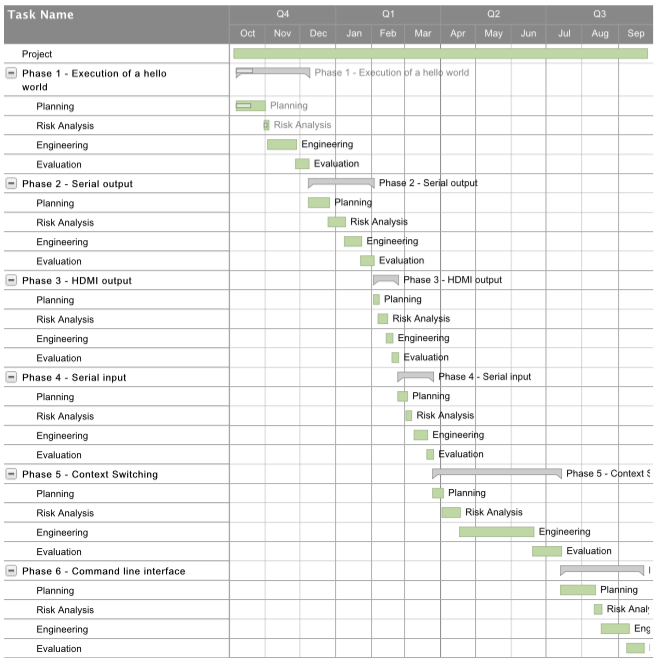
\includegraphics[width=1\textwidth]{includes/figures/chapter7_gant_diagram.png}  \\[0.5 cm]
\end{center}
\caption{Gant Chart of the Project}
\label{fig:chapter7_gant_diagram}
\end{figure}


\section{Cost Projection}

This section is aimed to perform an estimation of the physical resources needed and their related amount of money spent throughout the realization of the project. It is necessary to take into account the deprecation of the material being used. The project being realized in Spain, we will refer to the country's law dedicated the mater, that is the \textit{Ley del impuesto de sociedades}\cite{ley_impuesto_sobre_sociedades}. The amortization\cite{amortizacion_2015} of a computer is of \textit{8 years}. We will consider both the Raspberry Pi and the MacBook Pro to fall into that category.

As seen from the previous section, the project spans between eleven and twelve months, for our deprecation calculation we will therefore use a full year.

\begin{center}
\begin{table}[H]
    \centering
    \begin{tabular}{| p{2cm} | p{3.4cm} | p{3.4cm}| p{3.4cm} |}
    \hline
    \textbf{Material}        & \textbf{Cost for one unit}  & \textbf{Deprecation}& \textbf{Total for one year}\\\hline
    Personal computer       & \EUR{1500}                  & 8 years                     & \EUR{187,5} \\\hline
    Raspberry Pi B+         & \EUR{30}                    & 8 years                     & \EUR{3,75} \\\hline
    \multicolumn{3}{| p{8.8cm} |}{\textbf{Total}} & \textbf{\EUR{191,25}}\\ \hline
    \end{tabular}
    \caption{Cost projection for physical resources taking into account deprecation}
    \label{tbl:chapter7_cost_project_deprecation}
\end{table}
\end{center}



In terms of fungible resources, only electricity has been used. A MacBook Pro 13" uses about 12,1 Watts\cite{macbookpro_13_2013_energy_consumption}. A Raspberry Pi consumes about 1,21 Watts\cite{raspberry_pi_bplus_energy_consumption}. For a total of 13,31 Watts. Finally, the price per kWh is estimated to be \EUR{0,138280}\cite{tarifas_gas_luz}

We estimate the amount of average work of 17 hours a week with these devices, a total of 952 hours. We therefore can estimate the amount of energy spent to be \textit{12.67112kWh}. We can therefore estimate the amount of electricity spent to \textbf{\EUR{1,76}}.


Finally, we need to draw the cost of human resources. The amount of hour spent by each member can be obtained from the previous section. The table \ref{tbl:chapter7_human_resources_cost} shows the amount spent for each member.

\begin{center}
\begin{table}[H]
    \centering
    \begin{tabular}{| p{2cm} | p{3.4cm} | p{3.4cm}| p{3.4cm} |}
    \hline
    \textbf{Member}         & \textbf{Cost per hour} & \textbf{Hours worked}  & \textbf{Total}\\\hline
    Project Manager         & \EUR{35}             & 120 hours                & \EUR{4 200} \\\hline
    Requirement Engineer    & \EUR{20}             & 60 hours                & \EUR{1 200} \\\hline
    Analyst                 & \EUR{25}             & 80 hours                & \EUR{2 000} \\\hline
    Designer                & \EUR{25}             & 150 hours                & \EUR{3 750} \\\hline
    Developer               & \EUR{20}             & 210 hours                & \EUR{4 200} \\\hline
	Tester                  & \EUR{15}             & 110 hours                & \EUR{1 650} \\\hline
    \multicolumn{3}{| p{8.8cm} |}{\textbf{Total}} & \textbf{\EUR{17 000}}\\ \hline
    \end{tabular}
    \caption{Human resource cost}
    \label{tbl:chapter7_human_resources_cost}
\end{table}
\end{center}


With all these data, we can obtain the final cost of the project:


\begin{center}
\begin{table}[H]
    \centering
    \begin{tabular}{| c | c |}
    \hline
    \textbf{Concept}   & \textbf{Cost} \\ \hline
    Physical Resources	& \EUR{191,25} \\ \hline
	Fungible Resources & \EUR{1,76} \\ \hline
    Human Resources    & \EUR{17 000} \\ \hline
    Risk (15\%)        & \EUR{2 578,96} \\ \hline
    \textbf{Total without Tax}     & \textbf{\EUR{19 771,97}}\\ \hline
    Taxes 				& \EUR{3 954,394} \\ \hline
    \textbf{Total with Tax} & \textbf{\EUR{23 726,364}} \\ \hline
    \end{tabular}
    \caption{Cost Projection Total}
    \label{tbl:chapter7_total_cost_projection}
\end{table}
\end{center}


\chapter{Conclusions and lines of work}

This final section aims to conclude the work performed in this bachelor thesis project, underline the goals, experiences and impressions. In a second part of this conclusion, several lines of work are given for a future project based on this one. 

\section{Conclusions}

The major goal of this Bachelor Thesis was to implement a understandable and modular kernel dealing with a device on the bare metal level. It has been possible to implement more than what was initially planned. Several satisfying milestone were reached: Execute arbitrary code on the board, initialization of a serial connection with another device, dealing with graphic card concept and output data on the screen, handling input from a user and the most interesting one: Context switching. This later has been the hardest part if we exclude the initial study of the Raspberry Pi. Context switching are simple on the paper but harder to implement and overall to debug on a bare metal level, which make it even more satisfying when finally finding the solution.

This project has been very interesting has many things weren't seen during the degree but many concepts of what has been studied could and have been be applied. The adventure through low level programming made me realize how interesting, yet difficult, this world is as there are no security policy or advanced debug tool to prevent the program to write on forbidden addresses. The whole process was a lot of study and research of the Raspberry Pi board, ARM processor, cross-compiler, assembler and more advanced concept of computer science. Finally, the implementation was a lot of trial and error mitigated by the automated functional testing from the library, which was impossible to be used when the code reached a too close-to-the-metal level. Testing on the board is impossible until having basic outputs (a blinking LED at first and finally serial outputs), debugging getting more easy as the tools are getting built.

In the end, I believe that we can say that the initial goals of the project were reached with a satisfying outcome.


\section{Future works}

The project, although being a solid base, lacks of many functionality that modern operating systems employ.
A main research direction is a feature that were planned at first was to develop Virtual Memory for the process, allowing them not to step on each other toes and overall to render safe a process from another one. This involves implementing a module translating the address from virtual memory to physical memory.

Another direction is also the implementation of a file system. None is included in this project and every program or data need to be included within the kernel at compilation time, no data can be retrieved from the SD Card. This would require the implementation of a FAT-32 driver (the file system in which the SD Card needs to be formatted to in order allow the firmware to boot from it) in the kernel.

The kernel is also devoid of USB support as it was too ambitious for the project, USB standards being more than 200 pages. An interesting feature would be to implement USB drivers in order to use an external keyboard or flash drive.

Finally, there are no explicit system calls in the kernel, a good research direction would be to implement such feature into the kernel.

\backmatter
\begin{appendices}
\chapter{List of Acronyms}

\begin{itemize}
\item\textbf{API} - Application Program Interface
\item\textbf{ARM} - Advanced RISC Machines
\item\textbf{CLI} - Command Line Interface
\item\textbf{CPSR} - Current Program Status Register
\item\textbf{FIQ} - Fast Interrupt Request
\item\textbf{GPIO} - General Purpose Input/Output
\item\textbf{HDMI} - High-Definition Multimedia Interface
\item\textbf{IRQ} - Interrupt Request
\item\textbf{ISR} - Interrupt Service Routine (Interrupt Handler)
\item\textbf{JPEG} - Joint Photographic Experts Group
\item\textbf{LLVM} - Low Level Virtual Machine
\item\textbf{LR} - Link Register
\item\textbf{OS} - Operating System
\item\textbf{PCB} - Process Control Block
\item\textbf{PID} - Process ID
\item\textbf{PCIe} - Peripheral Component Interconnect Express
\item\textbf{PWM} - Pulse Width Modulator
\item\textbf{RISC} - Reduced Instruction Set Computer
\item\textbf{RPI} - Raspberry Pi
\item\textbf{RTOS} - Real-Time Operating System
\item\textbf{SATA} - Serial AT Attachment
\item\textbf{SoC} - System on Chip
\item\textbf{SPSR} - Saved Processor Status Register
\item\textbf{SP} - Stack Pointer
\item\textbf{SVC} - Supervisor
\item\textbf{TDD} - Test-driven development
\item\textbf{USB} - Universal Serial Bus
\end{itemize}
\bibliography{includes/tex/bibliography}{}
\bibliographystyle{plain}
\end{appendices}

\end{document}